\documentclass[12pt]{article}
\usepackage{hyperref}
\hypersetup{
    colorlinks=true,
    linkcolor=blue,
    filecolor=magenta,      
    urlcolor=blue,
}

\usepackage{import}
\import{"../Algebraic Geometry/"}{AlgGeoCommands}

\newcommand{\Loc}[1]{\mathfrak{Loc}\left( #1 \right)}
\newcommand{\AbGrp}{\mathbf{AbGrp}}
\usepackage{bbm}
\usepackage{cancel}
\usetikzlibrary{decorations.pathreplacing,calligraphy}


\begin{document}

\sloppy

\section{TODO!!}

\begin{enumerate}
\item Finish symplectic geometry course
\begin{enumerate}
\item figure out if symplectic toric is the same as projective toric variety (projectivity needed to come from a polytope and also to be Kahler)
\item review coisotropic reduced and write some notes
\item hyperkahler reduction examples 
\item are there examples of non-compact hyperkahlers?
\item work out the kinks in notes on Hamiltonian actions
\end{enumerate}
\item review killing homotopy groups Columbia lectures and write some notes
\item figure out those damn jet bundles and connections on principal bundles
\begin{enumerate}
\item RMK: $\pi^* E$ is NOT trivial for a vector bundle let alone a fiber bundle. it does get equipped with a canonical section but for a vector bundle this is just the trivial section, only for a principal bundle does giving a section trivialize it.
\item role of atiyah sequence vs jet bundle sequence
\item 
\end{enumerate}
\item spectral sequences for tor and ext in derived category (FIND MY NOTES ON THIS!)
\begin{enumerate}
\item application to universal coefficient theorem
\item Kunneth spectral sequence
\item Kunneth formula for smash product?
\item why are derived functors triangulated
\item derived functors in terms of Kan extensions (NOTES)
\end{enumerate}
\item write notes on universal morphisms
\item $G$-action of $X/Y$ induces map Descent data $X/Y$ to $G$-equivariant sheaves
\begin{enumerate}
\item isomorphism when $X/Y$ is a $G$-cover i.e. $X \to Y$ is a $G$-torsor
\item write down explicit $G$-equivariant structure on $\Omega_X$
\item Galois descent derive explicit form
\end{enumerate}
\item Weil restriction
\begin{enumerate}
\item write down trivialization after going back up
\item Galois descent in explicit form
\end{enumerate}
\item notes on Galois actions on schemes
\item notes on Frobenii
\item notes on universal constructions in math with examples

\item fix notes on Tor in category of sheaves and Tor symmetry (do I need symmetry of flat objects a priori?).

\item Finish stable homotopy theory course.

\item Finish vector bundles and connections notes (in AG folder)
\begin{enumerate}
\item Kahler iff $\nabla I = 0$ where $\nabla$ is the Levi-Civita connection
\item Ricci tensor and the trace bullshit 
\item Riemann-Hilbert and existence of flat frames for integrable connections
\end{enumerate}
\end{enumerate}

\section{What I Want to Think About}

\begin{enumerate}
\item Flat cohomology equal etale cohomology for smooth (affine groups) apply this to that counting rational points things
\item work out the details for the group fixing $\CC$ inside endomorphism group. What does an integrable structure of this kind look like, how close to a complex manifold can we get? In dimension two this should be exactly a conformal (not necessarily orientable) structure. 
\item FINISH CONFORMAL NOTES!
\item Hilbert Class Field of curves (ASK BRIAN FOR REFERENCE)
\item Read about Fredholm index and Riemann-Roch
\item Cohomology and inclusion-exclusion: cohomology for vectorspaces?
\end{enumerate}

\section{Some Questions I Have}

\begin{enumerate}
\item Reduction of structure group for a scheme.
\begin{enumerate}
\item what about the algebraic group $\mathrm{SL}^{\pm} = \det^{-1}(\mu)$ what does reduction of structure group give. For a manifold this is supposed to be a pseudo-volume form but obviously that's not right.
\item what about $\Res{\CC}{\RR}{\Gm} \embed \mathrm{GL}_2$ from the action $\Gm \acts \A^1_{\CC}$ restricted giving an action $\Res{\CC}{\RR} \Gm \acts \A^2_{\RR}$. I feel like this should give an almost complex structure. What properties does it have? What about for other fields?
\item What is an almost complex structure on a scheme look like?
\end{enumerate}
\item Is my calculation of an ``almost almost complex structure'' as reduction of structure group to $\left< \sigma \right> \ltimes \mathrm{GL}(n, \CC) \subset \mathrm{GL}(2n, \RR)$. For the case $n = 1$ this should be the conformal group justifying that I think this should correspond to the non-oriented case of a complex manifold since Riemann surfaces are exactly oriented conformal manifolds.
\end{enumerate}


\section{Project}

\section{Foliations}

\subsection{Riemannian Foliations}

\begin{rmk}
Given a transverse metric $g_\F$ to a foliation $\F \subset T M$ we can always choose a metric $g$ on $M$ such that $g$ is bundle-like. Indeed, just choose a splitting $T M \cong \F \oplus Q$ and choose any metric on $\F$ then take the sum. 
\end{rmk}

\subsection{Holonomy}

\subsection{Linearization}

HOW IS THIS RELATED TO THE NORMAL BUNDLE?

\section{Finding A Leaf}

Recall that $A$ is the cokernel of $\Alb_F \to \Alb_X$.

\begin{enumerate}
\item $\dim{F} \ge \dim{\Alb_F}$ by [Kawamata, Thm. 1]

\item $\dim{A} \ge \dim{\Alb_X} - \dim{\Alb_F}$ by definition

\item hence, $\dim{A} \ge \dim{\Alb_X} - \dim{F}$

\item $\dim{A} + \dim{W} \le \dim{\Alb_X}$ by Popa-Schnell 

\item hence we conclude $\dim{W} \le \dim{\Alb_X} - \dim{A} \le \dim{F}$.
\end{enumerate}
However, $\dim{W} = \dim{F}$ by assumption. Therefore, every one of the above inequalities is an equality.
\bigskip\\
Therefore, there is an exact sequence,
\begin{center}
\begin{tikzcd}
0 \arrow[r] & H^0(Y, \Omega_Y^1) \arrow[r] & H^0(X, \Omega^1_X) \arrow[r] & H^0(F, \Omega^1_F) \arrow[r] & 0
\end{tikzcd}
\end{center}
The first map is injective by generic smoothness of $X' \to Y$ and the fact that Hodge numbers are birational invariants. The second map is surjection by (in)equality (b) and then the sequence is exact by (in)equality (c). 
\bigskip\\
Therefore, the image $W|_F \subset H^0(F, \Omega_F)$ is everything. But recall that $F \to \Alb_F$ is dominant by Kawamata. Therefore generically the global forms on $F$ span the cotangent space meaning the forms $W|_F$ are a generic coframe of $F$. This implies,
\[ X \to \Alb_X \to \Alb_X^\vee \to \Alb_F^\vee \]
is surjective because $\Alb_F \to \Alb_F^\vee$ is finite and any section of $H^0(X, \Omega_X^1) \onto H^0(F, \Omega^1_F)$ must generically span a $\dim{F}$ subspace of the cotangent space since these forms span $F$ at its generic point.

\section{Contracting Fibers}

\begin{prop}
Let $X, Y, A$ be varieties over $\CC$. Suppose there is a diagram,
\begin{center}
\begin{tikzcd}
X \arrow[r, "g"] \arrow[d, "f"] & A 
\\
Y
\end{tikzcd}
\end{center}
where $A$ is an abelian variety and $f,g$ are proper, $f$ is $\struct{}$-connected, and the general fiber of $f$ is an abelian variety which maps finitely onto its image under $g$. Then $g$ is a smooth isotrivial abelian fibration. (WHAT ABOUT IF Y IS SINGULAR) (POTENTIALLY GOOD REDUCTION!!) (OKAY SO THIS IS TRUE OUTSIDE OF CODIMENSION $2$ I THINK)
\end{prop}

(CAN I PROVE THAT EVERY FIBER IS AN ABELIAN VARIETY WITH POSSIBLY REDUCED STRUCTURE)

\begin{proof}
Let $y \in Y$ be a point with a singular fiber. Then choose a map $\Spec{R} \to Y$ from a DVR whose closed point hits $y$. Let $K = \Frac{R}$ then $X_K$ is a torsor over an abelian $K$-scheme so after some extension of DVRs $R' \supset R$ is becomes an abelian variety with semi-stable reduction. Let $\cA$ be the Neron model of $X_{K'}$ and consider the diagram,
\begin{center}
\begin{tikzcd}
\cA^\circ \arrow[rd] \arrow[r, dashed] & X_{R'} \arrow[d] \arrow[r] & X_{R} \arrow[d] \arrow[r] & X \arrow[d] \arrow[r] & A
\\
& \Spec{R'} \arrow[r] & \Spec{R} \arrow[r] & Y 
\end{tikzcd}
\end{center}
\end{proof}

\section{Stuff}

\begin{lemma}
Suppose we have a diagram of schemes,
\begin{center}
\begin{tikzcd}
X \arrow[rd] \arrow[r, dashed, "f"] & Y' \arrow[d, "g"]
\\
& Y
\end{tikzcd}
\end{center}
with $X$ normal and integral where $f : X \rat Y'$ is a rational map and $g : Y' \to Y$ is finite and $g \circ f$ is a morphism. Then $f$ is a morphism.
\end{lemma}

\begin{proof}
This is a local question on $X$ so shrinking $Y$ and then $X$ (and taking $Y'$ the preimage) we may assume that everything is affine. Therefore, we have the situation,
\begin{center}
\begin{tikzcd}
K \arrow[from=r] & A'
\\ 
R \arrow[u, hook] \arrow[from=r] & A \arrow[u] 
\end{tikzcd}
\end{center}
where $K = \Frac{R}$ and $A \to A'$ is finite. Since $A'$ is integral over $A$ its image in $K$ is integral over $R$ but $R$ is a normal domain so the image is contained in $R$ and hence we get a unique map $A' \to R$ proving the claim. 
\end{proof}

\section{Chow Stuff}

Let $X, Y, Z$ be smooth projective varieties over $k$. Recall that there exists a composition,
\[ \CH^{d}(Y \times Z) \times \CH^{d'}(X \times Y) \to \CH^{d+d' - \dim{Y}}(X \times Z) \]
given by,
\[ \Gamma_2 \circ \Gamma_1 = \pi_{13_*}(\pi_{12}^* \Gamma_1 \frown \pi_{23}^* \Gamma_2) \]

\begin{lemma}
This composition is associative.
\end{lemma}

\begin{proof}
Consider $\Gamma_1 \in \CH^{d}(X \times Y)$ and $\Gamma_2 \in \CH^{d'}(Y \times Z)$ and $\Gamma_3 \in \CH^{d''}(Z \times W)$. Then we get,
\begin{align*}
\Gamma_3 \circ (\Gamma_2 \circ \Gamma_1) &= \pi^{134}_{14 *} (\pi_{13}^{134*} (\Gamma_2 \circ \Gamma_1) \frown \pi_{34}^{134*} \Gamma_3)
\\
&= \pi^{134}_{14 *} (\pi_{13}^{134*} [\pi^{123}_{13*} (\pi^{123*}_{12} \Gamma_1 \frown \pi^{123*}_{23} \Gamma_2)] \frown \pi_{34}^{134*} \Gamma_3)
\\
&= \pi^{134}_{14 *} ( \pi^{1234}_{134*} \pi^{1234*}_{123} (\pi^{123*}_{12} \Gamma_1 \frown \pi^{123*}_{23} \Gamma_2) \frown \pi_{34}^{134*} \Gamma_3)
\\
&= \pi^{134}_{14 *} ( \pi^{1234}_{134*} (\pi^{1234*}_{12} \Gamma_1 \frown \pi^{1234*}_{23} \Gamma_2) \frown \pi_{34}^{134*} \Gamma_3)
\\
&= \pi^{134}_{14 *}  \pi^{1234}_{134*} ((\pi^{1234*}_{12} \Gamma_1 \frown \pi^{1234*}_{23} \Gamma_2) \frown  \pi^{1234^*}_{134} \pi_{34}^{134*} \Gamma_3)
\\
& = \pi^{1234}_{14*} ((\pi^{1234*}_{12} \Gamma_1 \frown \pi^{1234*}_{23} \Gamma_2) \frown  \pi^{1234^*}_{34} \Gamma_3)
\end{align*}
so we reduce to associativity for intersection product.
\end{proof}

There is also an action,
\[ \CH^{d}(X \times Y) \times \CH^{e}(Y) \to \CH^{e+d-\dim{X}}(X) \]
defined by,
\[ \Gamma^* \alpha = \pi_{1*} (\Gamma \frown \pi_2^* \alpha) \]
Likewise, there is a pairing,
\[ \CH^{d}(X \times Y) \times \CH^{e}(X) \to \CH^{e+d-\dim{Y}}(Y) \]
defined by,
\[ \Gamma_* \alpha = \pi_{2*}(\pi_1^* \alpha \frown \Gamma) \]
By the commutativity of intersection product, it is obvious that $\Gamma^* = (\Gamma^\top)_*$ where $(-)^\top$ is applying the involution $X \times Y \to Y \times X$.

\begin{lemma}
The above composition law makes this action functorial,
\[ (\Gamma_2 \circ \Gamma_1)_* \alpha = \Gamma_{2*} \Gamma_{1*} \alpha \]
and likewise,
\[ (\Gamma_2 \circ \Gamma_1)^* \alpha = \Gamma_2^* \Gamma_1^* \alpha \]
\end{lemma}

\subsection{Vanishing Lemmas}

Here we need that all varieties are non-singular and quasi-projective so we can apply the moving lemma.

\begin{defn}
Let $\alpha, \beta \in \CH^{\bullet}(X)$. We say that $\alpha, \beta$ meet \textit{properly} if for each variety $V$ and $W$ appearing in $\alpha$ and $\beta$ then,
\[ \dim{(V \cap W)} = \dim{V} + \dim{W} - \dim{X} \]
\end{defn}

\begin{theorem}[Moving Lemma]
If $X$ is non-singular and quasi-projective, and $\alpha, \beta$ are cycles on $X$ then there is $\alpha' \sim_{\text{rat}} \alpha$ such that $\alpha'$ and $\beta$ meet properly. 
\end{theorem}

\begin{prop}
Suppose that $\alpha, \beta \in Z^{\bullet}(X)$ are such that $\Supp{}{\alpha} \cap \Supp{}{\beta} = \empty$. Then $\alpha \frown \beta = 0$.
\end{prop}

\begin{proof}
On a nonsingular variety, we have $\alpha \frown \beta \in \CH_\bullet(\Supp{}{\alpha} \cap \Supp{}{\beta})$ if we use the ``refined product'' in terms of Gysin maps (which does not meaningfully differ from $\iota^*$ in the case of regularly embedded subvarieties) see [Fulton, p. 131].
\end{proof}

\begin{lemma}
Suppose that $\Supp{}{\Gamma} \subset X \times V$ where $\codim{V,X} = r$ then $\Gamma^* \alpha = 0$ for all $\alpha \in \CH^{e}(Y)$ where $e > \dim{Y} - r$. 
\end{lemma}

\begin{proof}
It suffices to consider $\Gamma$ and $\alpha$ prime divisors. Then $\Gamma \subset X \times V$ and $\pi_2^* \alpha = X \times \alpha$. Notice that the expected dimension of $V$ intersecting $\alpha$ is negative so by the moving lemma there exists $\alpha' \sim_{\text{rat}} \alpha$ disjoint from $V$. Therefore, $(X \times V) \cap (X \times \alpha) = \empty$ and thus $\Gamma \frown \pi_2^* \alpha = 0$.
\end{proof}


\begin{prop}
The diagram,
\begin{center}
\begin{tikzcd}
\CH^{d}(Y \times Z) \times \CH^{d'}(X \times Y) \arrow[d, "\ell", two heads] \arrow[r] & \CH^{d+d' - \dim{Y}}(X \times Z) \arrow[d, two heads, "\ell"]
\\
\CH^{d}(Y \times_k Z) \times \CH^{d'}(k(X) \times_k Y) \arrow[r, dashed] & \CH^{d+d' - \dim{Y}}(k(X) \times_k Z) 
\end{tikzcd}
\end{center}
induces a well-defined composition law. 
\[ \CH^{d}(Y \times Z) \times \CH^{d'}(Y_{k(X)}) \to \CH^{d+d'-\dim{Y}}(Z_{k(X)}) \]
\end{prop}

\begin{proof}
We need to show if $\delta' \in \ker{\ell_{X,Y}}$ then $\Gamma' \circ \delta' \in \ker{\ell_{X,Z}}$. It suffices to consider the case of prime cycles (since being in the kernel is a condition only on the support which passes to each prime component of a cycle) so assume $\delta'$ is a prime cycle with $\Supp{}{\delta} \subset D \times Y$ then,
\[ \Gamma' \circ \delta' = \pi_{13*}(\pi_{12}^* \delta' \frown \pi_{23}^* \Gamma') \]
but $\delta' \subset D \times Y$ so $\Gamma' \circ \delta' \subset D \times Z$ and hence is in the kernel. 
\end{proof}

\begin{rmk}
This is just given by pullback after base changing along $k(X) / k$. Indeed $\pi_{23}^*$ is just base change along $L / k$ for the cycle $\Gamma$ after passing to $(Y \times Z)_{L}$ and $\pi_{12}^*$ is just pullback along the first projection $(Y \times Z)_{L} \to Y_{L}$. This works for any field $L/k$ as used in the proof of [Voisin, Birational Invariants, Prop. 2.9]. 
\end{rmk}

\begin{example}
Consider $X = Y = Z = \P^2$ and $\Gamma_1 = \ell \times X$ and $\Gamma_2 = X \times \ell$. Then,
\[ \Gamma_2 \circ \Gamma_1 = \pi_{13*}( (X \times \ell \times X) \frown (X \times \ell \times X)) = X \times X \]
which is nonzero in $\CH^0(k(X) \times_k X)$. However, $\ell(\Gamma_1) = 0$ by definition. This shows that,
\[ \CH^{1}(k(X) \times_k X) \times \CH^{1}(k(X) \times_k X) \to \CH^{0}(k(X) \times_k X) \]
is \textit{not} well-defined. This is because we are pairing in $\CH^{1}$ not $\CH_{0}$. However, we will see that $\CH_0(X_K)$ acts on $\CH^{d}(X_K)$.
\end{example}

\begin{prop}
The diagram,
\begin{center}
\begin{tikzcd}
\CH^{d}(Y \times Z) \times \CH^{\dim{X}}(X \times Y) \arrow[d, "\ell", two heads] \arrow[r] & \CH^{d + r}(X \times Z) \arrow[d, two heads, "\ell"]
\\
\CH^{d}(k(Y) \times_k Z) \times \CH_{0}(k(X) \times_k Y) \arrow[r, dashed] & \CH^{d + r}(k(X) \times_k Z) 
\end{tikzcd}
\end{center}
where $r = \dim{X} - \dim{Y}$ induces a well-defined composition law. 
\end{prop}

\begin{proof}
We need to show if $\delta \in \ker{\ell_{Y,Z}}$ then $\delta \circ \Gamma \in \ker{\ell_{X,Z}}$ since we already showed the other composition is well-defined. It suffices to consider the case of prime cycles (since being in the kernel is a condition only on the support which passes to each prime component of a cycle) so assume $\delta$ is a prime cycle with $\Supp{}{\delta} \subset D \times Z$ and $\Gamma \subset X \times Y$ is a prime cycle then,
\[ \delta \circ \Gamma = \pi_{13*}(\pi_{12}^* \Gamma \frown \pi_{23}^* \delta) \]
We can assume that $\Gamma$ is a prime cycle dominating $X$ else this is automatically in $\ker{\ell_{X,Z}}$ by the previous proposition. Therefore, $\Gamma$ is the graph of a correspondence,
\begin{center}
\begin{tikzcd}
& \Gamma \arrow[dl, "\pi"'] \arrow[rd, "f"] 
\\
X & & Y
\end{tikzcd}
\end{center}
where $\pi$ is generically finite. If $\pi_{12}^* \Gamma \frown \pi_{23}^* \delta$ does not dominate $X$ then it will be in the kernel so we can assume that $\im{f} \subset D$ otherwise the support of the intersection will be contained in $f^{-1}(D) \times D \times Z$ and $f^{-1}(D)$ is a proper closed subset of $\Gamma$ and hence cannot dominate $X$. Then we apply the moving lemma to find $\Gamma' \sim_{\text{rat}} \Gamma$ such that $\Gamma'$ intersects $X \times D$ properly. Then passing to the irreducible components of $\Gamma'$ which, as before, we can assume dominate $X$ then by pure dimension count $\Gamma' \frown (D \times X)$ cannot dominate $X$ and hence $\delta \circ \Gamma = 0$.
\end{proof}

\begin{rmk}
Note, that the other direction does \textit{not} hold. We don't get a well-defined map for,
\begin{center}
\begin{tikzcd}
\CH^{\dim{Y}}(Y \times Z) \times \CH^{d'}(X \times Y) \arrow[d, "\ell", two heads] \arrow[r] & \CH^{d'}(X \times Z) \arrow[d, two heads, "\ell"]
\\
\CH_0(k(Y) \times_k Z) \times \CH^{d'}(k(X) \times_k Y) \arrow[r, "\xcancel{--}" description] & \CH^{d'}(k(X) \times_k Z) 
\end{tikzcd}
\end{center}
Indeed, consider $X = Y = Z = \P^2$ then consider, $\delta = [\ell \times \ell] \in \CH^2(X \times X)$ and $\Gamma = [X \times \ell] \in \CH^1(X \times X)$. Since $\delta$ is zero in $\CH_0(X_K)$ the composition $\delta \circ \Gamma$ should be in the kernel. However, 
\[ \delta \circ \Gamma = \pi_{13*}([X \times \ell \times X] \frown [X \times \ell \times \ell]) = [X \times \ell] \]
which is nontrivial in $\CH_1(X_K)$. The asymmetry here is quite strange. In $\CH^{\dim{X}}{X \times X}$ we have well-defined pullbacks and pushforward of cycles. However, $\CH_0(X_K)$ only has a well-defined pullback, there is no pushforward. This is related to the asymmetry where the transpose of a cycle on $\CH^{d}(X \times X)$ is not a well-defined operation at the level of $\CH_0(X_K)$ e.g. consider $[X \times *]$ vs $[* \times X]$, one is zero the other is nonzero in $\CH_0(X_K)$. 
\end{rmk}

(WHAT ABOUT $\ell(\Gamma^\top)$ vs $\ell(\Gamma)$. THIS COULD BE VERY DIFFERENT!!)

\subsection{Ring Structure}

\begin{rmk}
$\Hom{\rat}{X}{Y}$ is the set of dominant rational maps $X \rat Y$. Therefore is is equivalent to maps $k(Y) \to k(X)$ in the category of fields over $k$. The category of varieties with dominant rational maps is equivalent to the category of finitely-generated fields over $k$.
\end{rmk}

\begin{prop}
The diagram,
\begin{center}
\begin{tikzcd}
\Hom{\rat}{Y}{Z} \times \Hom{\rat}{X}{Y} \arrow[d] \arrow[r] & \Hom{\rat}{X}{Z} \arrow[d]
\\
\CH_0(k(Y) \times_k Z) \times \CH_0(k(X) \times_k Y) \arrow[r] & \CH_0(k(X) \times_k Z)
\end{tikzcd}
\end{center}
commutes.
\end{prop}

\begin{proof}
Let $f : X \rat Y$ and $g : Y \rat Z$ be rational maps. First, if $f$ and $g$ are morphisms then $\Gamma_g \circ \Gamma_f = \Gamma_{g \circ f}$ so the claim is obvious. Let $U \subset X$ and $V \subset Y$ be open subsets such that $f : U \to V$ and $g : V \to Y$ are morphisms. Therefore,
\[ (\pi_{12}^* \Gamma_f \frown \pi_{23}^* \Gamma_g)|_{U \times V \times Z} = [\im{(\id, f, g \circ f)}|_{U}] \]
Therefore, 
\[ \alpha = (\pi_{12}^* \Gamma_f \frown \pi_{23}^* \Gamma_g) - [\overline{\im{(\id, f, g \circ f)}|_{U}}] \]
has support on $(U \times V \times Z)^C$. Any term supported on $U^C \times Y \times Z$ does not dominate $X$ and hence will be zero in $\CH_0(k(X) \times_k Z)$. Therefore, it suffices to consider terms supported on $X \times V^C \times Z$. We can assume each prime cycle $\alpha$ dominates $X$ and hence $\alpha \frown \pi_{1}^*(x)$ is nonzero for any $x \in X$. However, $\pi_1^*(x)$ intersects both $(\pi_{12}^* \Gamma_f \frown \pi_{23}^* \Gamma_g)$ and $[\overline{\im{(\id, f, g \circ f)}|_{U}}]$ is degree $\deg{x}$ (since they are birational onto $X$ and by the projection formula $\pi_{1*}(\Gamma \frown \pi_{1}^*(x)) = \pi_{1*} \Gamma \frown [x] = [X] \frown [x] = [x]$ so $\deg{(\Gamma \frown \pi_{1}^*(x))} = \deg{[x]}$). Therefore $\alpha$ does not dominate $X$ proving the claim. (FIND A BETTER PROOF).
\end{proof}

\newcommand{\RatEnd}[1]{\mathrm{RatEnd}\left( #1 \right)}

\begin{cor}
The map $\RatEnd{X} \to \CH_0(X_K)$ is a ring map. 
\end{cor}


\section{Curves on Fanos}

\newcommand{\Def}[1]{\mathrm{Def}\left( #1 \right)}
\newcommand{\Ob}[1]{\mathrm{Ob}\left( #1 \right)}
\newcommand{\ob}{\mathrm{ob}}

\begin{theorem}
Let $X$ be a smooth projective separably rationally connected variety over an algebraically closed field $k$. Then $X$ is connected by genus $g$ curves of arbitrary moduli for each $g \ge 0$. Explicitly, for each integer $g \ge 1$ there exists a map from a family of smooth proper irreducible genus $g$ curves,
\begin{center}
\begin{tikzcd}
\C \arrow[d] \arrow[r] & X 
\\
B
\end{tikzcd}
\end{center}
with $B$ a finite type $k$-scheme equipped with two sections $\sigma_1, \sigma_2 : B \to \C$ such that,
\begin{enumerate}
\item the general fiber of $\C \to B$ is unramified (embedded if $\dim{X} \ge 3$) under $\C \to X$ 

\item the map,
\[ B \xrightarrow{(\sigma_1, \sigma_2)} X \times X \]
is dominant and the fibers $(\sigma_1, \sigma_2)^{-1}(x_1, x_2)$ dominate $\M_{g,2}$ under the map $B \to \M_{g,2}$.
\end{enumerate} 
\end{theorem}

\begin{rmk}
For $g = 0$ the statement is vacuous for the silly reason that $\overline{\M}_{0,2} = \empty$. The corresponding statements about passing rational curves through points is well-studied (e.g. Kollar, Rational Curves on Algebraic Varieties) and will be essential in the proof.
If $k$ is not algebraically closed then we can make the same construction for $X_{\bar{k}}$ and $B$ will be defined over some finite $k'/k$. This is really necessary, since $X$ could have no $k$-point. 
\end{rmk}

\begin{proof}
We consider the moduli space,
\[ \overline{\M}_{g,n}(X ; d,  x_1, \dots, x_r) \]
for integers $g,n,r$ with $r \le n$ of maps from stable curves $f : C \to X$ of genus $g$ with $n$ marked points such that $p_i \mapsto x_i$ for $i \le r$ for fixed point $x_1, \dots, x_r \in X$ and such that $f_* C \cdot H \le d$ for a choice of ample divisor $H$. Note that this stack is proper (in particular has finitely many irreducible components) over $k$. It will suffice to show that for any pair of point $x_1, x_2 \in X$ the map $\overline{\M}_{g,n}(X, x_1, x_2) \to \overline{\M}_{g,n}$ has a nonempty smooth locus containing a closed point which is an embedded curve in $X$. This implies the map to $\overline{\M}_{g,n}$ is dominant (its image contains a nonempty open) and a generic member of $\overline{\M}_{g,n}(x_1, x_2)$ is embedded since this is an open condition. Indeed, we conclude via the following diagram,
\begin{center}
\begin{tikzcd}
& \overline{\M}_{g,n}(X ; d, x_1, x_2) \arrow[r] \arrow[d] & (x_1, x_2) \arrow[d]
\\
B \arrow[r, "\et"] & \overline{\M}_{g,n}(X ; d) \arrow[d] \arrow[r, "\sigma_1 \times \sigma_2"] & X \times X 
\\
& \overline{\M}_{g,n}
\end{tikzcd}
\end{center}
where $B \to \overline{\M}_{g,n}(X ; d)$ is an \etale map from finite type $k$-scheme chosen to dominate each component of $\overline{\M}_{g,n}(X ; d)$ containing the point of $\overline{\M}_{g,n}(X ; d, x_1, x_2)$ at which the map to $\overline{\M}_{g,n}$ is smooth. Then the family of curves over $B$ satisfies the required properties because the general fiber of $B \to X \times X$ maps to $\overline{\M}_{g,n}$ with a nonempty smooth locus and hence dominates. Therefore, we reduce to the following lemma.
\end{proof}

\begin{lemma}
With the above notation, for each $g \ge 1$ and $n \ge 2$ there exists $d > 0$ such that for all pairs $x_1, x_2 \in X$ the map,
\[ \overline{\M}_{g,n}(X ; x_1, x_2) \to \overline{\M}_{g,n} \]
has a nonempty smooth locus.
\end{lemma}

\begin{proof}
We will probe this question via relative infinitesimal deformation theory. Let,
\[ \mu_0 = [C_0, f_0, p_1, \dots, p_n] \in \overline{\M}_{g,n}(X; d, x_1, x_2)(k) \]
be a fixed point and $c_0 = [C, p_1, \dots, p_n] \in \overline{M}_{g,n}(k)$ its image. Then for each small extension of Artin local $k$-algebras,
\begin{center}
\begin{tikzcd}
0 \arrow[r] & I \arrow[r] & A' \arrow[r] & A \arrow[r] & 0
\end{tikzcd}
\end{center}
we need to fill in any lifting diagram,
\begin{center}
\begin{tikzcd}
\Spec{A} \arrow[d] \arrow[r] & \overline{\M}_{g,n}(X; x_1, x_2) \arrow[d]
\\
\Spec{A'} \arrow[r] \arrow[ru, dashed] & \overline{\M}_{g,n}
\end{tikzcd}
\end{center}
to be $2$-commutative if $\Spec{k} \to \Spec{A'} \to \overline{\M}_{g,n}$ is $c_0$ (i.e. is equipped with a $2$-morphism). Heuristically, there is an exact sequence,
\begin{center}
\begin{tikzcd}
\Aut{c_0} \arrow[r] & \Def{f_0} \arrow[r] & \Def{\mu_0} \arrow[r] & \Def{c_0} \arrow[r] & \Ob{f_0}
\end{tikzcd}
\end{center}
and we need to show that $\Def{\mu_0} \onto \Def{c_0}$ is surjective so it suffices to show that,
\[ \Ob{f_0} = \Ext{1}{C}{f^* \Omega_{X}}{\struct{C}(-p_1-p_2) \ot I} \]
is zero. 
Explicitly, given a deformation $[C, p_1, \dots, p_n]_{A'}$ of $c_0$ over $A'$ and and a map $f_A : C_A \to X$ we need to extend the map to $f_{A'} : C \to X$ fixing the points $p_1, p_2$. By lemma \ref{def_theory} there is an obstruction,
\[ \ob (f_A) \in \Ext{1}{C}{f^* \Omega_X}{\struct{C_0}(-p_1 - p_2) \ot I} = \Ext{1}{C_0}{f_0^* \Omega_X}{\struct{C_0}(-p_1-p_2)} \ot_k I \]
Therefore, it suffices to find a $c_0$ with the requisite vanishing property which we do in the following proposition. 
\end{proof}

\begin{prop}
With the above notation, for each $g \ge 1$ there is a $d \ge 0$ so that there exist an unramified (embedded) stable curve $\mu_0 = [C, f, p_1, \dots, p_n] \in \overline{\M}_{g,n}(X ; d, x_1, x_2)$ for some $n \ge 2$ such that,
\[ \Ext{1}{C}{f^* \Omega_X}{\struct{C}(-p_1 - p_2)} = H^1(C, f^* \T_X(-p_1-p_2)) = 0 \]
\end{prop}

\begin{proof}
Repeatedly applying the following lemma (and taking $d = g d(g+3)$) we can find an immersed (embedded if $\dim{X} \ge 3$) stable curve, $[C, x_1, x_2, p_1, \dots, p_{g+1}] \in \overline{\M}_{g, g+3}(X; d, x_1, x_2)$, 
\begin{center}
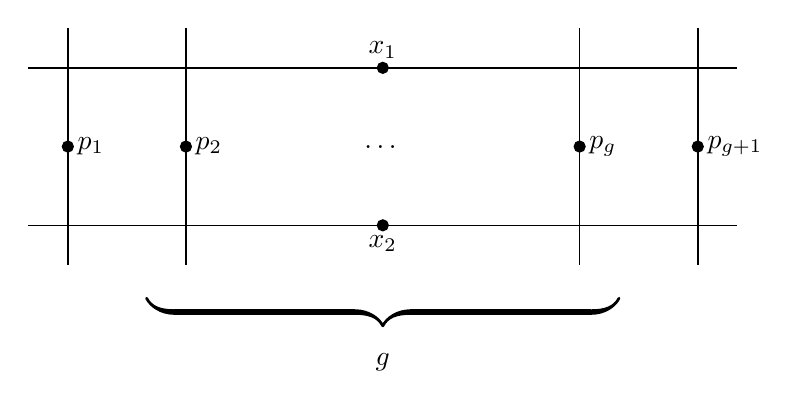
\begin{tikzpicture}

    
	\draw[line width=0.2mm] (0,0) -- (0,3);
	\filldraw[black] (0, 1.5) circle (2pt)
	node[anchor=west]{$p_1$};
	
    \draw[line width=0.2mm] (1.5,0) -- (1.5,3);
   	\filldraw[black] (1.5, 1.5) circle (2pt)
	node[anchor=west]{$p_2$};

    \node at (4, 1.5) {\dots} ;    
    
    \draw[line width=0.2mm] (6.5,0) -- (6.5,3); 
   	\filldraw[black] (6.5, 1.5) circle (2pt)
	node[anchor=west]{$p_g$};
    \draw[line width=0.2mm] (8,0) -- (8,3);
   	\filldraw[black] (8, 1.5) circle (2pt)
	node[anchor=west]{$p_{g+1}$};
    
    
    \draw[line width=0.2mm] (-0.5,0.5) -- (8.5,0.5);
	\draw[line width=0.2mm] (-0.5,2.5) -- (8.5, 2.5);
	
   	\filldraw[black] (4, 2.5) circle (2pt)
	node[anchor=south]{$x_1$};
		
   	\filldraw[black] (4, 0.5) circle (2pt)
	node[anchor=north]{$x_2$};
	

% Calligraphic brace
\draw [decorate, line width = 2pt,
    decoration = {calligraphic brace,mirror, raise=5pt, amplitude = 10pt}] (1,-0.25) --  (7, -0.25) ;
    \node[anchor=north] at (4, -1) {$g$};
 
 	
\end{tikzpicture}
\end{center}
We use the prescribed tangent directions to ensure that each node is immersed (i.e. the branches do not become tangent in the image) and the lemma says that each component is immersed (embedded if $\dim{X} \ge 3$). Furthermore, if $\dim{X} \ge 3$ we can take $Z$ to be the union of the curves we have constructed up to this point and ensure that each new curve only intersects $Z$ in $X$ at the two prescribed points. Therefore, we get an embedding $f : C \to X$ of the above stable curve.
\bigskip\\
It suffices to compute the obstruction space. Applying Lemma \ref{ext_vector_bundle} we need to show that,
\[ H^0(\wt{C}, \nu^* f^* \T_X(-x_1 - x_2)) \to \bigoplus_{x \in C^{\sing}} T_{x} X \]
is surjective. However, $\nu^* f^* \T_X(-x_1 - x_2)$ restricted to each vertical component is just the pullback of $\T_X$ along a very free  curve $f : \P^1 \to X$ (since $x_1, x_2$ only lie on the horizontal components) and hence is ample. Therefore, its evaluation at any two distinct points is surjective. Since each node is on unique vertical components and there are only two nodes on each vertical components we see that the evaluation map to the nodes is surjective.
\end{proof}

\begin{lemma}
Let $B \subset \P^1$ be a finite subscheme of length $b$. Let $f : \P^1 \to X$ be a rational curve,
\[ f^* \T_X \cong \bigoplus_{i = 1}^n \struct{\P^1}(a_i) \]
with $a_1 \ge a_2 \ge \cdots \ge a_n$. Then,
\begin{enumerate}
\item if $a_2 > b$ and $f|_B$ is unramified the general deformation of $f$ fixing $f|_B$ is unramified

\item if $a_3 > b$ and $f|_B$ is an embedding the general deformation of $f$ fixing $f|_B$ is an embedding.
\end{enumerate}
\end{lemma}

\begin{proof}
To appear.
\iffalse
For part (a) it suffices to deform $f$ along a tangent field $H^0(\P^1, f^* \T_X \ot \I_B)$ which vanishes nowhere except on $B$. Since $a_2 > b$ thus $f^* \T_X \ot \I_B$ contains two copies of $\struct{\P^1}(a_i)$ with $a_i > 0$. (WHY DONT GET IT WITH JUST $a_1 \ge b$ SINCE THEN HAVE A FREE PARAMETER AND MAKE IT VANISH COMPLETELY ALONG $B$) (WHAT ABOUT OBSTRUCTIONS)

By part (a) we can deform $f$ such that it is unramified. Then factoring $f : \P^1 \to \P^1 \to C$ through the normalization we must have the first map be an isomorphism or else by Riemann-Hurwitz it would have ramification. Thus $f$ is an immersion with finitely many ordinary multiple points. We need to deform $f$ along a tangent field $H^0(\P^1, f^* \T_X \ot \I_B)$ which separates the branches at these multiple points.  
\fi
\end{proof}

\begin{rmk}
We will make use of [Kollar, IV Thm. 3.9]. Combining this with the explicit degree bounds for smoothing combs (c.f. [Kollar, IV Thm. 3.10]) we conclude that there exists an integer $d(n)$ such that every finite set of points of length $n$ lies on an unramified (embedded) very free rational curve of $H$-degree at most $d(n)$.
\end{rmk}

\begin{lemma}
Let $X$ be smooth, projective, separably rationally connected variety over $k = \bar{k}$. For each ample divisor $H$, there exists an integer $d(n) \ge 0$ such that for all,
\begin{enumerate}
\item closed subschemes $Z \subset X$ with $\codim{Z, X} \ge 2$ 

\item distinct closed points $x_1, \dots, x_n \in X$ 

\item tangent directions $\ell_i \in T_{x_i} X$ 
\end{enumerate}
Then there exists a rational curve $f : \P^1 \to X$ such that,
\begin{enumerate}
\item $f_* [\P^1] \cdot H \le d$

\item $f$ is very free meaning $f^* \T_X$ is ample

\item $f$ is immersed (unramified and $f(\P^1)$ has only nodal singularities) and embedded if $\dim{X} \ge 3$

\item $x_1, \dots, x_n \in f(\P^1)^{\smooth}$ and $f(\P^1) \sm \{ x_1, \dots, x_n \}$ is disjoint from $Z \sm \{ x_1, \dots, x_n \}$

\item if $t_1, \dots, t_n \in \P^1$ satisfy $t_i \mapsto x_i$ then $f_* : T_{t_i} \P^1 \to T_{x_i} \P^1$ is an isomorphism onto $\ell_i \cdot k$.
\end{enumerate}
\end{lemma}

\begin{proof}
To appear.
\end{proof}

\subsection{Ext on Stable Curves}

\begin{lemma} \label{ext_vector_bundle}
Let $C$ be a nodal curve and $\E$ a vector bundle on $C$. Suppose that on the normalization of each component $C_i \subset C$ the vector bundle $\E$ satisfies $H^1(\wt{C}_i, \E|_{\wt{C}_i}) = 0$ then,
\[ H^1(C, \E) = 0 \iff H^0(\wt{C}, \nu^* \E) \onto \bigoplus_{x \in C^{\sing}} \E(x) \text{ is surjective} \]
\end{lemma}

\begin{proof}
Let $\nu : \wt{C} \to C$ be the normalization. Consider the exact sequence,
\begin{center}
\begin{tikzcd}
0 \arrow[r] & \E \arrow[r] & \nu_* \nu^* \E \arrow[r] & \bigoplus\limits_{x \in C^{\sing}} \iota_{x*} \E(x) \arrow[r] & 0 
\end{tikzcd}
\end{center}
Let $\wt{\E} = \nu^* \E$ then the second map is defined as follows. For the two preimages $\wt{x}_1, \wt{x}_2 \in \nu^{-1}(x)$ of a node $x \in C^{\sing}$, the second map seconds a section $s \in \Gamma(\wt{U}, \wt{\E})$ to the difference,
\[ s(\wt{x}_1) - s(\wt{x}_2) \in \E(x) \]
under the canonical identifications,
\begin{center}
\begin{tikzcd}
\wt{\E}(\wt{x}_1) \arrow[rr, "\sim"] \arrow[rd, "\sim"] & & \wt{\E}(\wt{x}_2) \arrow[ld, "\sim"']
\\
& \E(x)
\end{tikzcd}
\end{center}
Then taking the long exact sequence we get,
\begin{center}
\begin{tikzcd}[column sep = small]
0 \arrow[r] & H^0(C, \E) \arrow[r] & \bigoplus\limits_{C_i \subset C} H^0(\wt{C}_i, \wt{\E}|_{\wt{C}_i}) \arrow[r] & \bigoplus\limits_{x \in C^{\sing}} \E(x) \arrow[r] & H^1(C, \E) \arrow[r] & \bigoplus\limits_{C_i \subset C} H^0(\wt{C}_i, \wt{\E}|_{\wt{C}_i}) \arrow[r] & 0
\end{tikzcd}
\end{center}
and thus we conclude.
\end{proof}

\begin{prop}
COMBINATORICS OF SPLITTING TYPE ON A NODAL CURVE WITH RATIONAL COMPONENTS, DO THIS.
\end{prop}

\subsection{Deformation Theory}

\begin{lemma} \label{def_theory}
Let $A$ be an Artin local ring with residue field $\kappa$. Let $X_A$ be a smooth $A$-scheme and $C_A, B_A$ be any $A$-schemes and the data,
\begin{enumerate}
\item $A$-morphisms $g_A : B_A \to C_A$ and $f_A : C_A \to X_A$ with $g_A$ a closed embedding

\item a small extension of Artin local rings,
\[ 0 \to I \to A' \to A \to 0 \]

\item deformations $B_{A'}$ of $B_A$ and $C_{A'}$ of $C_A$ and $X_{A'}$ of $X_A$ over $A'$

\item deformations $g_{A'} : B_{A'} \to C_{A'}$ of $g_A$ and $h_{A'}$ of $h_{A} = f_A \circ g_A$
\end{enumerate}
then, denoting the data over $\kappa$ with a $0$, there exists a class,
\[ \ob(f_A) \in \Ext{1}{C_0}{f_0^* \Omega_{X_0}}{\I_{B_0}} \ot_k I \]
obstructing the existence of a map $f_{A'} : C_{A'} \to X_{A'}$ such that $f_{A'} \circ g_{A'} = h_{A'}$ where,
\[ \I_{B_0} = \ker{(\struct{C_0} \to g_{0*} \struct{B_0})} \]
\end{lemma}

\begin{proof}
Using the flatness properties, we need to consider the following lifting problem,
\begin{center}
\begin{tikzcd}
& & g_* \struct{B_{A'}} \arrow[from=dd, bend left = 70, near start, "h_{A'}^{\#}"] \arrow[r] & g_* \struct{B_A}
\\
0 \arrow[r] & I \ot \struct{C_0} \arrow[r, crossing over] & \struct{C_{A'}} \arrow[u] \arrow[r] & \struct{C_A} \arrow[r] \arrow[u] & 0
\\
& & f^{-1}_0 \struct{X_{A'}} \arrow[u, dashed]  \arrow[r] & f^{-1}_0 \struct{X_A} \arrow[u, "f_A^{\#}"] 
\end{tikzcd}
\end{center}
such that the diagram commutes. The set of such liftings locally on $C_0$ is a torsor over,
\[ \Der[A']{f_0^{-1} \struct{X_{A'}}}{\I_{B_0} \ot_\kappa I} = \Der[k]{f_0^{-1} \struct{X_0}}{\I_{B_0}} \ot_\kappa I = \shHom{\struct{C_0}}{f_0^* \Omega_{X_0}}{\I_{B_0}} \ot_\kappa I \]
Therefore, it suffices to show that lifts exist locally. The local picture,
\begin{center}
\begin{tikzcd}
0 \arrow[r] & I \ot B_0 \arrow[r] & B' \arrow[from=dd, bend left = 70] \arrow[r] & B \arrow[r] & 0
\\
0 \arrow[r] & I \ot S_0 \arrow[u] \arrow[r, crossing over] & S' \arrow[u] \arrow[r] & S \arrow[r] \arrow[u] & 0
\\
& I \ot J_{B_0} \arrow[u] & R' \arrow[u, dashed, "\ell'"] \arrow[r] & R \arrow[u, "\ell"] 
\\
& 0 \arrow[u]
\end{tikzcd}
\end{center}
where $R'$ is smooth over $A'$ so there exists a lift $\ell' : R \to S'$ over $A'$ since $S' \to S$ is a square-zero extension. We need to modify the lift to make it commute with $R' \to B'$. The difference is an element $\delta \in \Hom{R'}{\Omega_{R'/A'}}{B_0 \ot_\kappa I}$  
so we consider the exact sequence,
\begin{center}
\begin{tikzcd}
\Hom{R'}{\Omega_{R'}}{S_0 \ot_\kappa I} \arrow[r] & \Hom{R'}{\Omega_{R'}}{B_0 \ot_\kappa I} \arrow[r] & \Ext{1}{R'}{\Omega_{R'/A'}}{J_{B_0} \ot_\kappa I}
\end{tikzcd}
\end{center}
which arises from tensoring the exact sequence (using that $g_A$ is a closed embedding for surjectivity)
\begin{center}
\begin{tikzcd}
0 \arrow[r] & J_{B_0} \arrow[r] & S_0 \arrow[r] & B_0 \arrow[r] & 0
\end{tikzcd}
\end{center}
by $- \ot_\kappa I$ which remains exact since $\kappa$ is a field and applying $\Hom{R'}{\Omega_{R'/A'}}{-}$. Now $\Omega_{R'/A'}$ is a projective $R'$-module so the Ext is zero and hence we can lift $\delta$ to a derivation $\tilde{\delta} : R' \to S_0 \ot_\kappa I$ then $\ell' - \tilde{\delta}$ gives the required lift. 
\end{proof}

\begin{rmk}
We can weaken the hypothesis that $g$ is a closed embedding. However, we still need some condition. Indeed, consider deformations of a line mapping to a line through a point but we deform the image of the line off of the point. Explicitly, consider the deformations over $k[\epsilon]$,
\begin{center}
\begin{tikzcd}
k[\epsilon, y] \arrow[r] & k[y]
\\
k[\epsilon] \arrow[u] \arrow[r] & k \arrow[u]
\\
k[\epsilon, x] \arrow[uu, bend left = 60, "x \mapsto \epsilon y"] \arrow[u, dashed,  "\xcancel{-}" description] \arrow[r] & k[x] \arrow[u, "x \mapsto 0"']
\end{tikzcd}
\end{center}
Any maps $k[\epsilon, x] \to k[\epsilon, z]$ making the diagram commute must send $x$ into $\epsilon k[\epsilon, z]$ but this maps inside $k[\epsilon] \subset k[\epsilon, y]$ and hence does not make the left triangle commute. Therefore, some condition on the map $h_{A'} : B_{A'} \to X_{A'}$ is required. It is clearly necessarily to assume that $\im{h_{A'}^{\#}} \subset \im{g_{A'}^{\#}}$ because for there to be a factorization,
\begin{center}
\begin{tikzcd}
S' \arrow[rr] & & B'
\\
& R' \arrow[ru, dashed] \arrow[lu]  
\end{tikzcd}
\end{center}
it is of course necessary that $\im{(R' \to B')} \subset \im{(S' \to B')}$. However, we need slightly more in general as the next example shows,
\begin{center}
\begin{tikzcd}
k[\epsilon, y] \arrow[r] & k[y]
\\
k[\epsilon, z] \arrow[u, "z \mapsto \epsilon y"'] \arrow[r] & k[z] \arrow[u, "z \mapsto 0"']
\\
k[\epsilon, x] \arrow[uu, bend left = 60, "x \mapsto \epsilon y"] \arrow[u, dashed,  "\xcancel{-}" description] \arrow[r] & k[x] \arrow[u, "x \mapsto 0"']
\end{tikzcd}
\end{center}
Any map $k[\epsilon, x] \to k[\epsilon, z]$ making the diagram commute must send $x$ into $\epsilon k[\epsilon, z]$ but this lands inside $k[\epsilon] \subset k[\epsilon, y]$ under $k[\epsilon, z] \to k[\epsilon, y]$ and hence does not make the left triangle commute. Heuristically, the composition of two first-order deformations of a constant map should be non-constant only to second-order and thus cannot equal a non-trivial first-order deformation of the composed constant map. The issue algebraically is that $\ker{(k[\epsilon, z] \to k[\epsilon, y])} = (\epsilon, z^2)$ does not surject onto $(z) = \ker{(k[z] \to k[y])}$ which is exactly needed to make such liftings possible\footnote{Diagram chasing by first sending $x \mapsto \bar{x}$ to an element making the left triangle commute we then need to modify the image so that its projection in $k[z]$ is correct. It may not be correct but it is correct after mapping to $k[y]$ since the outer square commutes so we need to kill an element of $\ker{(k[z] \to k[y])}$. Thus, we need to modify $\bar{x}$ by something in $\ker{(k[\epsilon, z] \to k[\epsilon, y])}$ (to not change the left triangle commuting) to hit a specified element of $\ker{(k[z] \to k[y])}$. Thus we need the required surjectivity.} 
\bigskip\\
The right conditions are:
\begin{enumerate}
\item $\im{h_{A'}^{\#}} \subset \im{g_{A'}^{\#}}$

\item $\ker{g_{A'}^{\#}} \onto \ker{g_{A}^{\#}}$ is surjective (e.g. when $\ker{g_{A'}^{\#}}$ is $A'$-flat, so true when $g_{A'}$ is an embedding).
\end{enumerate}

The proof is modified as following. We need to show that the difference $\delta' : R' \to B_0 \ot_\kappa I$ lands in $\im{(S_0 \to B_0)} \ot_\kappa I$ (equals $\im{(S_0 \ot_\kappa I \to B_0 \ot_\kappa I)}$ since $\kappa$ is a field). By the first assumption $\delta$ has image inside $\im{(S' \to B')} \cap \ker{(B' \to B)}$. Applying the snake lemma to the diagram,
\begin{center}
\begin{tikzcd}
0 \arrow[r] & I \ot B_0 \arrow[r] & B' \arrow[r] & B \arrow[r] & 0
\\
0 \arrow[r] & I \ot S_0 \arrow[u] \arrow[r, crossing over] & S' \arrow[u] \arrow[r] & S \arrow[r] \arrow[u] & 0
\end{tikzcd}
\end{center}
we get an exact sequence,
\begin{center}
\begin{tikzcd}
\ker{(S' \to B')} \arrow[r] & \ker{(S \to B)} \arrow[r, "\partial"] & \coker{(S_0 \to B_0)} \ot_\kappa I \arrow[r] & \coker{(S' \to B')} 
\end{tikzcd}
\end{center}
Then $\delta$ maps to $\coker{(S_0 \to B_0)} \ot_\kappa I$ and has zero image in $\coker{(S' \to B')}$ since its image lies inside $\im{(S' \to B')}$. By the second hypothesis, the connecting map $\partial = 0$ since the map on kernels is surjective so the image of $\delta$ in $\coker{(S_0 \to B_0)} \ot_\kappa I$ is zero giving us what we want. Thus we get $\delta : R' \to \im{(S_0 \to B_0)} \ot_\kappa I$ and hence we can apply the exact sequence,
\begin{center}
\begin{tikzcd}
\Hom{R'}{\Omega_{R'}}{S_0 \ot_\kappa I} \arrow[r] & \Hom{R'}{\Omega_{R'}}{\im{(S_0 \to B_0)} \ot_\kappa I} \arrow[r] & \Ext{1}{R'}{\Omega_{R'/A'}}{J_{B_0} \ot_\kappa I}
\end{tikzcd}
\end{center}
which arises from tensoring the exact sequence,
\begin{center}
\begin{tikzcd}
0 \arrow[r] & J_{B_0} \arrow[r] & S_0 \arrow[r] & \im{(S_0 \to B_0)} \arrow[r] & 0
\end{tikzcd}
\end{center}
by $- \ot_\kappa I$ which remains exact since $\kappa$ is a field and applying $\Hom{R'}{\Omega_{R'/A'}}{-}$. Now $\Omega_{R'/A'}$ is a projective $R'$-module so the Ext is zero and hence we can lift $\delta$ to a derivation $\tilde{\delta} : R' \to S_0 \ot_\kappa I$ then $\ell' - \tilde{\delta}$ gives the required lift.
\end{rmk}

\section{Smoothing Singularities}

\begin{theorem}
Let $X_0$ be a $k$-scheme and $X$ a deformation of $X_0$ over $C$,
\begin{enumerate}
\item there are three successive obstructions to the existence of an extension $X'$ over $C'$,
\[ \ob_1 \in H^0(X_0, \T^2_{X_0} \ot J) \quad \ob_2 \in H^1(X_0, \T^1_{X_0} \ot J) \quad \ob_3 \in H^2(X_0, \T^0_{X_0} \ot J) \]

\item If these obstructions are zero then there is a sequence,
\begin{center}
\begin{tikzcd}
0 \arrow[r] & H^1(X_0, \T^0_{X_0} \ot J) \arrow[r] & \Def{X, C'} \arrow[r] & H^0(X_0, \T^1_{X_0} \ot J) \arrow[r] & H^2(X_0, \T^0_{X_0} \ot J)
\end{tikzcd}
\end{center}
\end{enumerate}
\end{theorem}

\begin{rmk}
Therefore, if we find an example with smoothable singularities where $\T^2_{X_0} = 0$ and $\T^1_{X_0}$ supported in dimension zero (i.e. isolated lci singularities) but the map,
\[ H^0(X_0, \T^1_{X_0} \ot J) \to H^2(X_0, \T^0_{X_0} \ot J) \]
is nontrivial then we could have singularities which can be individually smoothed but not simultaneously. 
\bigskip\\
However, this never happens if $\dim{X_0} = 0$. We see that curves with isolated lci singularities are always smoothable. Indeed, there is no obstruction and,
\[ \Def{X, C'} \onto H^0(X_0, \T^1_{X_0} \ot J) \]
is surjective. There is no obstruction to deforming an ample line bundle so we can use formal GAGA to algebrize this deformation. Now the claim is that every lci singularity is individually smoothable. SEE \chref{https://arxiv.org/pdf/0808.0436.pdf}{TRY}.
\end{rmk}

\section{Relative Kawamata}

\begin{example}
Let $E$ be an elliptic curve and $C$ any curve with a $G$-cover of $\P^1$. Let $G$ act on $E$ by translation. Then we get,
\[ X = (E \times C) / G \to E/G \times C/G = E' \times \P^1 \]
is finite. However, $X \to \P^1$ is not a smooth isotrivial fibration. Indeed, it has double fibers over the ramification points of the map $C \to \P^1$. 
\end{example}

\begin{rmk}
From this example, it seems that double fibers ``is the worst you get'' with $X$ smooth. Is this actually true? What about for $X$ normal? Say if $X$ has terminal singularities and is $\Q$-Cartier as well? 
\end{rmk}

\section{Amazing $K$-theory Facts}

\begin{prop}[Quillen, Higher $K$-Theory I]
Let $X$ be a noetherian scheme and $G_i(X)$ the $K$-theory of the category of coherent sheaves. Then there is a spectral sequence,
\[ E^{p,q}_1 = \prod_{x \in X^{(p)}} K_{-p-q}(\kappa(x)) \implies G_{-(p+q)}(X) \]
where $X^{(p)}$ is the set of codimension $p$ points.
\end{prop}

\subsection{Milnor $K$-Theory}

\begin{prop}[Totaro, Milnor K-Theory is the Simplest Part of Algebraic K-Theory]
There are isomorphisms,
\[ K_n(X) \ot \Q \cong \bigoplus_p \CH^p(X, n) \ot \Q \]
but integrally the RHS behaves more like Milnor $K$-theory. Indeed, if $F$ is a field then,
\[ \CH^p(F, n) = 0 \quad p > n \]
and,
\[ \CH^n(F, n) = H^n(F, \Z(n)) = K^M_n(F) \]
where the middle group is motivic cohomology.
\end{prop}

\begin{theorem}[Bloch-Kato]
If $r$ is invertible in the field $F$ then there is an isomorphism,
\[ K^M_n(F) / r \iso H^n_{\et}(F, \Z / r \Z(n)) \]
\end{theorem}



\subsection{Log Differential Forms}

\begin{defn}
The sheaf $W_n \Omega^i_{X, \log}$ is the \etale subsheaf of $W_n \Omega^i_X$ generated by terms of the form,
\[ \log{\ul{x}_1} \wedge \cdots \wedge \log{\ul{x}_i} \]
for $x_1, \dots, x_i \in \struct{X}^\times$. We set $W_n \Omega^i_{X, \log} = 0$ for $n \le 0$.
\end{defn}

\begin{rmk}
Here, underline is the (not homomorphism) $k \to W(k)$ sending an element to the Witt vector $(x, 0, \cdots, 0)$.
\end{rmk}

\begin{rmk}
For th case $n = 1$, Milne offers a different definition. 
\end{rmk}

There is a Cartier operation,
\[ C : Z \Omega^r_{X/S} \to \Omega^r_{X/S} \]
where $Z \Omega^r_{X/S}$ denotes the closed $r$-forms. Then we define as a sheaf on $X_{\et}$,
\[ \Omega^r_{X, \log} = \ker{(1 - C)} \]
In fact, the sequence,
\begin{center}
\begin{tikzcd}
0 \arrow[r] & \Omega^r_{X, \log} \arrow[r] & Z \Omega^r_{X/S} \arrow[r, "1 - C"] & \Omega^r_{X/S} \arrow[r] & 0
\end{tikzcd}
\end{center}
in the \etale topology. 

\begin{rmk}
WHY DOES ALL THIS NEED THE ETALE TOPOLOGY. PROBABLY NOT SURJECTIVE OTHERWISE!
\end{rmk}

\begin{prop}[\chref{https://www.imo.universite-paris-saclay.fr/~jean-louis.colliot-thelene/CTSansucSoule.pdf}{Lemma 3}]
There are exact sequence,
\begin{center}
\begin{tikzcd}
0 \arrow[r] & W_n \Omega^r_{X, \log} \arrow[r, "\times p^m"] & W_{n+m} \Omega^r_{X, \log} \arrow[r, "R^n"] & W_m \Omega^r_{X, \log} \arrow[r] & 0
\end{tikzcd}
\end{center}
where $R$ is the natural projection operator and $\times p^m$ means the map such that its precomposition under $R^m$ is multiplication by $p^m$ on $W_{n+m} \Omega^r_{X, \log}$.
\end{prop}

DOES THIS ALLOW US TO COMPUTE COHOMOLOGY OF $W_2$ I THINK SO! NEED TO KNOW COHOMOLOGY OF $\Omega^i_{X, \log}$.

\section{Cartier Operator}

\chref{http://www.numdam.org/item/10.24033/asens.1309.pdf}{Milne's Paper}

\begin{defn}
The Cartier operator $C : Z\Omega^r_{X/S} \to \Omega^r_{X/S}$ is uniquely defined by,
\begin{enumerate}
\item $C(1) = 1$

\item $C(f^p \omega) = f C(\omega)$ for $f \in \struct{X}$ and $\omega \in Z\Omega^r_{X/S}$

\item $C(\omega \wedge \omega') = C(\omega) \wedge C(\omega')$ for closed points

\item $C(\omega) = 0$ iff $\omega$ is exact

\item $C(f^{p-1} \d{f}) = \d{f}$.
\end{enumerate}
\end{defn}

\begin{rmk}
Note that,
\[ C(\d{\log}(f)) = C \left( \frac{\d{f}}{f} \right) = C \left( \frac{f^{p-1} \d{f}}{f^p} \right) = \frac{\d{f}}{f} \]
by (b) and (e).
\end{rmk}

\begin{rmk}
Milne claims that every form is \etale locally a sum of exact forms and things of the form $f^{p-1} \d{f}$. 
\bigskip\\
For example, consider on $X = \P^1$ the form representing $H^1(X, \Omega_X)$,
\[ \omega = \left( \frac{x_0}{x_1} \right) \d \left( \frac{x_1}{x_0} \right) \]
This is of the form $\frac{\d{f}}{f}$ so $C(\omega) = \omega$. Then considering the exact sequence of \etale sheaves,
\begin{center}
\begin{tikzcd}
0 \arrow[r] & \Omega^1_{X, \log} \arrow[r] & \Omega^1_{X} \arrow[r, "1 - C"] & \Omega^1_X \arrow[r] & 0
\end{tikzcd}
\end{center}
since $Z \Omega^1_X = \Omega^1_X$. Therefore, since $\Omega^1_X$ is coherent \etale cohomology computes Zariski topology,
\begin{center}
\begin{tikzcd}[column sep = small]
0 \arrow[r] & H^0(X, \Omega_{X, \log}^1) \arrow[r] & 0 \arrow[r] & 0 \arrow[r] & H^1(X, \Omega^1_{X, \log}) \arrow[r] & H^1(X, \Omega_X^1) \arrow[r, "1 - C"] & H^1(X, \Omega_X^1) \arrow[r] & H^2(X, \Omega_{X, \log}^1) \arrow[r] & 0
\end{tikzcd}
\end{center}
But $C(\omega) = \omega$ so the map $1 - C$ is zero. Hence we see,
\[ H^i(X, \Omega^1_{X, \log}) = 
\begin{cases}
0 & i = 0 \text{ or } i > 2
\\
k \cdot \omega & i = 1, 2
\end{cases} \]
\end{rmk}

\begin{example}
Let $X \subset \P^3$ be the degree $4$ Fermat surface over $\FF_3$. Then $\Omega_X^2 \cong \struct{X}$ with global section,
\[ \omega = \left( \frac{x_0^6}{x_1^3} \right) \d \left( \frac{x_2}{x_0} \right) \wedge \d \left( \frac{x_3}{x_0} \right) + \left( \frac{x_0^6}{x_2^3} \right) \d \left( \frac{x_1}{x_0} \right) \wedge \d \left( \frac{x_3}{x_0} \right) + \left( \frac{x_0^6}{x_3^3} \right) \d \left( \frac{x_1}{x_0} \right) \wedge \d \left( \frac{x_2}{x_0} \right) \] 
We also know that,
\[ H^i(X, \omega_X) = 
\begin{cases}
k \omega & i = 0
\\
0 & i = 1 \text{ or } i > 2
\\
k \eta & i = 2
\end{cases} \]
we need to work out the form representing the top Cech class. HOW DO I DO THIS, RATHER NOT.
\end{example}

\subsection{Cohomology of de Rham - Witt Complex}

\chref{https://projecteuclid.org/journals/arkiv-for-matematik/volume-22/issue-1-2/On-the-multiplicative-properties-of-the-de-RhamWitt-complex-I/10.1007/BF02384380.full}{Ekedahl - On the multiplicative properties of the de Rham—Witt complex. I}.

\begin{prop}
Let $X$ be proper and $N = \dim{X}$. For all $(i, j)$ the map,
\[ H^i(X, W_n \Omega^j) \iso \Hom{W_n}{H^{N-i}(X, W_n \Omega^{N-j})}{W_n} \]
is an isomorphism.
\end{prop}

\begin{example}
Let $X \subset \P^3$ be the degree $4$ Fermat over $\FF_3$. Then,
\[ H^i(X, W_2 \Omega^2) \iso \Hom{W_2}{H^{2-i}(X, W_2 \Omega^{0})}{W_2} \]
and $W_2 \Omega^0 = W_2 \struct{X}$ fits into an exact sequence,
\begin{center}
\begin{tikzcd}
0 \arrow[r] & \struct{X} \arrow[r] & W_2 \struct{X} \arrow[r] & \struct{X} \arrow[r] & 0
\end{tikzcd}
\end{center}
then we get in cohomology two extensions,
\begin{center}
\begin{tikzcd}
0 \arrow[r] & k \arrow[r] & H^0(X, W_2 \struct{X}) \arrow[r] & k \arrow[r] & 0
\\
0 \arrow[r] & k \arrow[r] & H^2(X, W_2 \struct{X}) \arrow[r] & k \arrow[r] & 0
\end{tikzcd}
\end{center}
we need to figure out the extension classes.
since both are modules over $W_2(k)$ my guess is this means,
\[ H^i(X, W_2 \struct{X}) = 
\begin{cases}
W_2(k) & i = 0,2
\\
0 & \text{else}
\end{cases} \]
Therefore, 
\[ H^0(X, W_2 \Omega^2) = \Hom{W_2}{H^2(X, W_2 \struct{X})}{W_2} = W_2(k) \]
which seems like exactly what we want paired with the following result.
\end{example}

\chref{https://arxiv.org/abs/1605.01913}{Torsion-orders of complete intersections}.


\begin{lemma}[Lemma 7.1]
Let $k$ be a perfect field of positive characteristic $p$ and $X, Y$ smooth equidimensional quasi-projective $k$-schemes. Let $n = \dim{X}$ and,
\[ \CH^n_{\mathrm{prop}/Y}(X \times Y) = \dlim_{Z} \CH_{\dim{Y}}(Z) \]
computed over subsets $Z \subset X \times Y$ proper over $Y$. For $\alpha \in \CH^n_{\mathrm{prop} / Y}(X \times Y)$ then we denote,
\[ \alpha_* : \bigoplus_{i,j} H^i(X, W_m \Omega^j) \to \bigoplus_{i,j} H^i(Y, W_n \Omega^j) \]
Assume that $\alpha$ is supported on $A \times Y$ where $A \subset X$ is a closed subscheme of codimension $\ge r$. Then $\alpha_*$ is zero on the direct summands with $j + r > n$.
\end{lemma}

Indeed, it seems that for $r = 1$ and $j = n$ we get that the action descends to $\CH_0(X_K)$. However, this is going to give a contradiction for the Fermat of degree $p+1$ since then we know that $p [\Delta] = 0$ in $\CH_0(X_K)$ because there is a degree $p$ cover $\P^2 \rat X$.


\section{Grassi-Wen}

\newcommand{\Bs}[1]{\mathrm{Bs}\left( #1 \right)}

\begin{theorem}
Let $\phi : X \to S$ be an elliptic fibration such that $X$ has $\Q$-factorial terminal singularities, $S$ is normal, and the canonical divisor $K_X = \phi^* L$ where $L$ is a $\Q$-CArtier divisor on $S$. Then there is a diagram,
\begin{center}
\begin{tikzcd}
X \arrow[d, "\phi"] \arrow[r, dashed, "\alpha"] & Y \arrow[d, "\psi"]
\\
S \arrow[from=r, "\beta"] & T
\end{tikzcd}
\end{center}
where $\alpha$ is a birational map, $\beta$ is a birational morphism, and $\psi$ is an elliptic fibration together with an effective $\Q$-divisor $\Lambda_T$ such that:
\begin{enumerate}
\item $Y$ has $\Q$-factorial terminal singularities
\item $K_Y = \psi^* (K_T + \Lambda_T) = \phi'^* L$ where $(T,\Lambda_T)$ is klt

\item there is no effective divisor $E \subset Y$ such that $\codim{\psi(E)} \ge 2$.
\end{enumerate}
\end{theorem}

\begin{proof}
Induction on the relative Picard number $\rho(X/S)$. Suppose that there is an integral divisor $E$ on $X$ such that $\codim{\phi(E)} \ge 2$. Then choose a Cartier divisor $C \subset S$ containing $\phi(E)$ such that the base locus $\Bs(|C|)$ is of codimension at least $2$, and $\psi^* C = D + F$ with $F$ the maximal component so that $\codim{\phi(F)} \ge 2$ and $D = \phi^* C - F$. Then $\supp{}{E} \subset \supp{}{F}$ and $\codim{\phi(D)} = 1$. Sinc
\end{proof}



Let $X$ be smooth good minimal model of $\dim{X} = n$ and $\kappa(X) = n - g$ with $\omega_1, \dots, \omega_g$ pointwise independent holomorphic $1$-forms. Let $\phi : X \to S$ to Iitaka fibration.
\begin{center}
\begin{tikzcd}
X \arrow[r, "\alpha_X"] \arrow[d, "\phi"] & \Alb_X
\\
S 
\end{tikzcd}
\end{center}
then $\alpha_X$ maps all fibers of $\phi$ to translates of a fixed subvariety $B \subset A_X$.

\subsection{Generalized Grassi-Wen}

Apply generalized Grassi-Wen (THIS ONLY USES LIE's RESULTS ON RELATIVE GOOD MINIMAL MODELS): we get birational modification,
\begin{center}
\begin{tikzcd}
X \arrow[from=r, dashed] \arrow[d, "\psi"] & Y \arrow[d, "\psi"]
\\
S \arrow[from=r] & T
\end{tikzcd}
\end{center} 
such that,
\begin{enumerate}
\item $Y$ has terminal $\Q$-factorial singularities
\item klt thing!!
\item codim thing
\end{enumerate}
additionally, want there exists an open $U \subset T$ such that,
\begin{enumerate}
\item $U$ is smooth

\item  $\codim{T \sm U, T} \ge 2$

\item $\psi|_U : Y_U \to U$ is equidim (easy, always true)

\item $\pi_1(Y_U) = \pi_1(X)$ (Generalized Grassi-Wen)

\item $Y_U \to U$ is a quasi bundle (all fibers of type $m A$ prob equivalent to lci and reduction is an abelian variety) (uses TAKAYAMA's RESULT) 

\item $Y_U$ is smooth.
\end{enumerate}

Claim that (a) + (b) + (c) implies (e). 

\begin{proof}
We are allowed to shrink $U$ by throwing out things smaller than divisors. Therefore we just need to show that $Y_U \to U$ does not have any divisors in its locus where the fibers are worse than multiple. This can be probed by general curves.
\bigskip\\
Take a general complete intersection curve $C = H_1 \cap \cdots \cap H_{n-g-1} \subset T$, claim that $\psi^{-1}(C) \subset Y$ is an irreducible normal and terminal variety. 
\begin{enumerate}
\item irreducible by Bertini: by induction on number of hyperplane cuts. We can assume $\dim{T} \ge 2$ then $| \psi^* H_i |$ is not a pencil therefore $\psi^{-1}(H_i)$ is irreducible 

\item normality: is also by induction. The general $\pi^{-1}(H_i)$ is lci in $Y$ (CHECK THIS!!!) and $\codim{\sing{\psi^{-1}(H_i))}} \ge 2$ and thus $\psi^{-1}(H_i)$ is normal.

\item terminal: Kollar-Mori lemma 5.17 discrepancy only goes up in general fiber. Therefore the fiber is terminal.
\end{enumerate}
Now we apply Takayama's results to see that $Y_C \to C$ is a quasi-bundle. 
\begin{center}
\begin{tikzcd}
\psi^{-1}(C) \arrow[d] \arrow[r, hook] & Y \arrow[d, "\psi"] \arrow[r, dashed] & X \arrow[r, "\alpha_X"] & A_X
\\
C \arrow[r] & T \arrow[r] & S
\end{tikzcd}
\end{center}
therefore, the fibers all map to translates of fixed thing in $A_X$ and are generically finite. This is used in the Takayama result. 
\bigskip\\
$K_Y$ is nef over $T$ so $Y_C \to C$ is relatively minimal (nef with respect to curves in the fibers). 
\bigskip\\
Therefore we have $F_1$ canonical and $K_{F_1} \sim_{\Q} 0$ and normal. Then $F_1 \to A$ generically finite and surjective. Thus $F_1$ is birational to abelian variety but $\kappa(F_1) = 0$ and thus $F_1$ is birational to an abelian variety.
\bigskip\\
Hover $F_1$ is already minimal since $K_{F_1} \sim_{\Q} 0$ so its isomorphic to an abelian variety.  
\end{proof}

Claim that this all implies (d):

\begin{proof}
Grassi-Wen will show this because no divisor $E$ on $Y$ is contracted to $\codim{\psi(Y)} \ge 2$. Therefore $Y_U \subset Y$ is a codim at least $2$ open. Used $Y$ is terminal so singularities have codim $3$
\end{proof}

Claim that this implies (f). 

\begin{proof}
$Y_U \to U$ we want to be smooth. In the elliptic fibration case we can just say the singular locus does not dominate $U$ since it is in codim $3$ and we can shrink somehow. This doesn't work for us.
\bigskip\\
Consider,
\begin{center}
\begin{tikzcd}
X \arrow[from=r, dashed, "\eta"] \arrow[d, "\phi"] & Y \arrow[d]
\\
S \arrow[from=r] & T
\end{tikzcd}
\end{center}
then $\eta$ is a sequence of flops by construction. If it becomes singular then the singular locus must be contained in a flopping locus. Given,
\[ Y \rat X_r \rat \cdots \rat X_1 \rat X \]
(DIM = 3 FlOPS DONT CHANGE SINGULARITIES BUT WE DONT KNOW FOR LARGER DIM). Flop is given by,
\[ X \to Z \]
small contration and then take $X^+$. Then $\sing{X^+} \subset \text{rulled subvariety} \subset X^+$ because this is an extremal contraction (contracting rational curves). Therefore, $Y_U \to Y$ is abelian fibration so every rulled subvariety of $Y$ must lie in the complement of 
\end{proof}

\section{LCI Things}

\begin{lemma}
Let $A \to B$ be a map of noetherian local rings with $A$ regular. Suppose that,
\[ \dim{B \ot \kappa(\m_A)} = \dim{B} - \dim{A} \]
and $B \ot \kappa(\m_A)$ is lci then $B$ is lci.
\end{lemma}

\begin{proof}
By \chref{https://stacks.math.columbia.edu/tag/09Q1}{Tag 09Q1} we reduce to the case that $A = k\dbrac{x_1, \dots, x_n}$ and $B$ is complete. Then consider,
\[ 0 \to I \to k\dbrac{x_1, \dots, x_n, y_1, \dots, y_r} \to B \to 0 \]
We assume that $B / (x_1, \dots, x_n)$ is lci meaning that $\bar{I}$ is generated by,
\[ q = r - (\dim{B} - n) = n + r - \dim{B} \]
elements. Choose a lift of the elements $f_1, \dots, f_q \in I$ which generate $\bar{I}$. Since $I$ is finitely generated and $\bar{f}_1, \dots, \bar{f}_q$ generate $\bar{I} / \m_B \bar{I} = I / \m_B I$ we see that $f_1, \dots, f_q \in I$ generate by Nakayama so we see that $B$ is lci. 
\end{proof}

\begin{cor} \label{lci_fibers_total_space_lci}
Let $X \to Y$ be a morphism of schemes with $Y$ regular such that every fiber $X_y$ is lci and pure dimension $\dim{X} - \dim{Y}$. Then $X$ is lci. 
\end{cor}

\begin{defn}
Let $(A, \m)$ be a Noetherian local ring. Let $X = \Spec{A}$ and $U = X \sm \{ \m \}$ be the punctured spectrum. We say $A$ \textit{satisfies purity} if the restriction functor,
\[ \FEt_X \to \FEt_{U} \]
is essentially surjective. 
\end{defn}

\begin{theorem}[SGA2 Expose X, Thm 3.4]
Let $A$ be a noetherian local ring suppose either,
\begin{enumerate}
\item $A$ is regular and $\dim{A} \ge 2$
\item $A$ is lci and $\dim{A} \ge 3$
\end{enumerate}
then $A$ satisfies purity. 
\end{theorem}

\begin{lemma}[\chref{https://stacks.math.columbia.edu/tag/0EY7}{Tag 0EY7}]
Let $j : U \embed X$ be an open immersion of Noetherian schemes such that purity holds for all $\stalk{X}{x}$ with $x \notin U$. Then,
\[ \FEt_X \to \FEt_U \]
is essentially surjective. 
\end{lemma}

\begin{lemma} \ref{birational_invariance_of_fund_group_lci}
Let $X, Y$ be normal projective $k$-varieties whose singularities are lci and supported in codimension $\ge 3$. A birational map $f : X \rat Y$ induces an isomorphism,
\[ f_* : \pi_1(X) \iso \pi_1(Y) \]
\end{lemma}

\newcommand{\dom}[1]{\mathrm{dom} \left( #1 \right)}

\begin{proof}
Let $W$ be a shared open of $X$ and $Y$ contained in $U = \dom{f} \subset X$ and $V = \dom{f} \subset Y$. Then we get a diagram,
\begin{center}
\begin{tikzcd}
& \pi_1(W) \arrow[ld, two heads] \arrow[rd, two heads]
\\
\pi_1(U) \arrow[d, "\sim"] & & \pi_1(V) \arrow[d, "\sim"] \arrow[lld, near start, "f^{-1}_*"'] 
\\
\pi_1(X) & & \pi_1(Y) \arrow[from=llu, near start, "f_*", crossing over]
\end{tikzcd}
\end{center}
The map $\pi_1(U) \to \pi_1(X)$ is an isomorphism because $X$ is normal and $Y$ is projective so $\codim{U, X} \ge 2$ so every $x \in X \sm U$ satsifies $\dim{\stalk{X}{x}} \ge 2$ and moreover if $x \in X^{\sing}$ then $\dim{\stalk{X}{x}} \ge 3$ and $\stalk{X}{x}$ is lci by assumption. Thus each $\stalk{X}{x}$ for $x \in X \sm U$ satisfies purity. Similarly, $\pi_1(V) \to \pi_1(Y)$ is an isomorphism. Therefore by commutativity of the diagram,
\[ \ker{(\pi_1(W) \onto \pi_1(X))} = \ker{(\pi_1(W) \to \pi_1(Y))} \]
so we conclude.
\end{proof}

Therefore we conclude.

\begin{prop}
Following our notation, 
\[ \pi_1(X) \iso \pi_1(Y_U) \]
\end{prop}

\begin{proof}
Indeed, $Y_U \to U$ satisfies the hypotheses of Cor \ref{lci_fibers_total_space_lci} and hence $Y_U$ is lci. Since $Y_U$ has $\Q$-factorial terminal singularities $\codim{Y_U^{\sing}, Y_U} \ge 3$ so we map apply lemma \ref{birational_invariance_of_fund_group_lci}. 
\end{proof}

\section{Deformation Complexes}

\newcommand{\LL}{\mathbb{L}}

\begin{defn}
Let $\X$ be a DM stack. Let $L^\bullet \in D(\struct{\X_{\et}})$. We say that, 
\begin{enumerate}
\item $L^\bullet$ is \textit{admissible} if,
\begin{enumerate}
\item $h^i(L^\bullet) = 0$ for all $i > 0$
\item $h^i(L^\bullet)$ is coherent for $i = 0,-1$.
\end{enumerate}
\item $L^\bullet$ is \textit{perfect} (with amplitude contained in $[a,b]$) if locally it quasi-isomorphic to a complex,
\[ 0 \to \E^a \to \cdots \to \E^b \to 0 \]
where each $\E^i$ is a vector bundle living in degree $i$. 
\end{enumerate}
\end{defn}

\begin{defn}
Let $E^\bullet \in D(\struct{\X_\et})$ be admissible. Then a homomorphism $\psi : E^\bullet \to \LL_{\X}$ is an \textit{obstruction theory} if,
\begin{enumerate}
\item $h^0(\phi)$ is an isomorphism
\item $h^{-1}(\phi)$ is surjective.
\end{enumerate}
\end{defn}

\begin{rmk}
Given a lifting problem,
\begin{center}
\begin{tikzcd}
T \arrow[r, "g"] \arrow[d, hook] & \X
\\
\ol{T} 
\end{tikzcd}
\end{center}
with ideal sheaf $\J$, we use the map $\phi$ to pullback the obstruction class $\omega(g) \in \Ext{1}{}{g^* \LL_{\X}}{\J}$ to an obstruction,
\[ \ob_{E}(g) := \phi^* \omega(g) \in \Ext{1}{}{g^* E^\bullet}{\J} \]
\end{rmk}


\begin{defn}
An obstruction theory $E^\bullet \to \LL_{\X}$ is \textit{perfect} if $E^\bullet$ is of perfect amplitude contained in $[-1,0]$.
\end{defn}

\begin{theorem}
The following are equivalence,
\begin{enumerate}
\item $\phi : E^\bullet \to \LL_{\X}$ is an obstruction problem

\item for any lifting problem $(T, \ol{T}, g)$ the obstruction $\ob_{E^\bullet}(g) \in \Ext{1}{}{g^* E^\bullet}{\J}$ vanishes if and only if there is a solution to the lifting problem and if $\ob_{E^\bullet}(g) = 0$ then the extensions form a torsor under $\Ext{0}{}{g^* E^\bullet}{\J} = \Hom{}{g^* h^0(E^\bullet)}{\J}$.
\end{enumerate}
\end{theorem}

\subsection{Examples}

\newcommand{\R}{\mathbf{R}}

\begin{example}
If $\X$ is smooth then $\LL_{\X}$ is a perfect deformation theory and there are no obstructions to lifting. 
\end{example}

\begin{example}
Let $C, X \to S$ be proper schemes. Consider the Hom scheme $\uHom{S}{C}{X}$ constructed from the Hilbert scheme. Recall that when $X$ is smooth, there is a classical tangent-obstruction theory,
\[ T^i = \Ext{i}{\struct{C}}{f^* \Omega_{X/S}}{\struct{C}} \]
to deforming a map $f : C \to X$ over $S$.
\bigskip\\
Let $H = \uHom{S}{C}{X}$ be the Hom scheme and consider the diagram,
\begin{center}
\begin{tikzcd}
H \times C \arrow[d, "\pi_1"] \arrow[r, "\ev"] & X
\\
C
\end{tikzcd}
\end{center}
Therefore we get maps,
\[ \ev^* \LL_{X} \to \LL_{H \times C} = \pi_1^* \LL_{H} \oplus \pi_2^* \LL_{C} \to \pi^*_1 \LL_{H} \]
using the functoriality of the cotangent complex. We want to push this forward to $H$ but the adjunction goes the wrong way. To fix this, we use Grothendieck duality. Assume that $C$ admits a dualizing complex $\omega_{C/S}^\bullet$. Then applying $- \ot^{\LL} \omega_{C/S}^\bullet$ we get,
\[ (\ev^* \LL_X) \ot^{\LL} \omega_{C/S}^\bullet \to (\pi_1^* \LL_{H}) \ot^{\LL}_{C/S} \iso \pi_1^! \LL_{H} \]
Now we can use the correct adjunction to get,
\[ \R \pi_* ([\ev^* \LL_{X}] \ot^{\LL} \omega_{C/S}^\bullet) \to \LL_{H} \]
Therefore, 
\[ E^\bullet = \R \pi_* ([\ev^* \LL_{X}] \ot^{\LL} \omega_{C/S}^\bullet) \]
is our candidate for an obstruction theory.
\end{example}

\begin{rmk}
This makes sense because we should be computing $\Ext{1}{\struct{C}}{f^* \Omega_X}{\struct{C}} = H^1(C, f^* \T_X)$ on the fibers in the smooth case where as $\R \pi_* \LL_{X}$ would be more like computing $H^1(f^* \Omega_X)$ on the fibers. In either case we will take $\RHom{}{-}{\struct{C}}$ on the base but this does not dualize $f^* \Omega_X$ to $f^* \T_X$ \textit{inside} the $\R \pi_*$.
\end{rmk}

\begin{theorem}
Let $S = \Spec{k}$. If $C$ is gorenstein then $E^\bullet \to \LL_{H}$ is an obstruction theory. If $C$ is a curve and $X$ is smooth the obstruction theory is perfect.
\end{theorem}

\begin{rmk}
IS GORENSTEIN REALLY NEEDED??
\end{rmk}

\begin{proof}
DO THIS!!!
\end{proof}

\begin{lemma}[Existence of the Mumford Complex]
Let $\pi : X \to S$ be a projective map 
\end{lemma}

\subsection{Moduli Stack of PRojective Varieties}

Let $\M$ and $\X$ be DM stacks and $p : \M \to \X$ be a flat relatively Gorenstein projective morphism (has constant relative dimension and that the relative dualizing complex $\omega_{\M/\X}^{\bullet}$ is a line bundle $\omega_{\M/\X}$. 
\bigskip\\
If $G^\bullet \in D^+(\struct{\X})$ when $p^! G^\bullet = p^* G^\bullet \ot^{\LL} \omega_{\M/\X}$ and thus for any complex $F^\bullet \in D^{-}(\struct{\M})$ there are natural isomorphisms,
\[ \Ext{k}{\struct{\M}}{F^\bullet}{p^* G^\bullet} \to \Ext{k}{\struct{\M}}{F^\bullet \ot^{\LL}}{p^! G^\bullet} \to \Ext{k}{\struct{\X}}{ \R p_* (F^\bullet \ot^{\LL} \omega_{\M/\X})}{G^\bullet} \]
The connecting map on cotangent complexes,
\[ \LL_{\M/\X} \to p^* \LL_{X}[1] \]
which we call the Kodaira-Spencer map since it reproduces it in the classical setting then induces a map,
\[ E^\bullet = \R p_* (\LL_{\M/\X} \ot^{\LL} \omega_{\M/\X}^\bullet)[-1] \to \LL_{\X}^\bullet \]

\begin{proof}
In the above situation. If $p : \M \to \X$ is \textit{universal} then $E^\bullet \to \LL^\bullet_X$ is an obstruction theory for $X$.
\end{proof}

\begin{proof}
DO THIS!!
\end{proof}

\begin{cor}
If $p$ is smooth of relative dimension $\le 2$ then $E^\bullet$ is a perfect obstruction theory. 
\end{cor}
\subsection{Cones}

\subsection{Construction of Virtual Fundamental Classes}


\begin{prop}
If $E^\bullet$ is a perfect obstruction theory with $h^0(E^\bullet)$ locally free and $h^1(E^\bullet) = 0$ then $X$ is smooth, the virtual dimension of $[X, E^\bullet]$ is $\dim{X}$ and $[X, E^\bullet] = [X]$.
\end{prop}

\begin{prop}
Let $X$ be smooth and $E^\bullet$ a perfect obstruction theory for $X$. If $h^0(E^\bullet)$ is locally free then the virtual fundamental class is,
\[ [X, E^\bullet] = c_r(h^1(E^{\bullet \vee})) \cdot [X] \]
where $r = \rank{h^1(E^{\bullet \vee})}$.
\end{prop}

\begin{proof}
If $F^\bullet \to E^\bullet$ is a global resolution of $E^\bullet$, then $C(F^\bullet) = \im{(F_0 \to F_1)}$.
\end{proof}



\newpage

\section{Fixing the Smoothness Problem}


\begin{prop}
Let $f : X \to \Spec{R}$ be a flat morphism over a dvr over an algebraically closed field $k$ of characteristic zero. Let $X_K \to \Spec{K}$ and $(X_0)_{\red} \to \Spec{\kappa}$ be smooth. Furthermore, assume that $X$ is normal\footnote{The second two conditions imply normality.}, lci, and $\codim{X^{\sing}} \ge 3$. Then $X$ is regular.
\end{prop}

\begin{proof}
Let $R' / R$ be a finite extension of dvrs such that $X(R')$ is nonempty. Consider,
\begin{center}
\begin{tikzcd}
\wt{X'} \arrow[r] \arrow[rd] & X' \pullback \arrow[d] \arrow[r] & X \arrow[d]
\\
& \Spec{R'} \arrow[r] & \Spec{R}
\end{tikzcd}
\end{center}
where $\wt{X'}$ is the normalization of $X'$. We will show that,
\begin{enumerate}
\item  $\wt{X'} \to X$ is \etale
\item  $\wt{X'} \to \Spec{R'}$ is smooth
\end{enumerate}
Given this, $\wt{X'}$ is regular and therefore $X$ is regular via the \etale covering. 
\bigskip\\
Since $X_0$ is lci, it has some well-defined multiplicity $m$. Explicitly, this means the map on complete local rings at a point $x \in X^{\smooth}$,
\begin{center}
\begin{tikzcd}
\stalk{X}{x} \arrow[from=d, hook] \arrow[r, hook] & \widehat{\stalk{X}{x}} \arrow[from=d, hook]
\\
R \arrow[r, hook] & k\dbrac{z}
\end{tikzcd}
\end{center}
satisfies $z \mapsto f^m$ where $f \in \widehat{\stalk{X}{x}}$ is irreducible\footnote{Note that $\stalk{X}{x}$ is regular and hence $\stalk{X}{x}$ is regular and thus a UFD. In general the completion of a UFD is \textit{not} a UFD so regularity here is essential.}. Therefore, since normalization and formal completion commute for excellent rings (see \chref{https://stacks.math.columbia.edu/tag/0C23}{Tag 0C23}) to show that $\wt{X'} \to X$ is \etale it suffices to perform the following local computation. At any $x' \in \wt{X'}$ with image $x \in X^{\smooth}$ consider,
\begin{center}
\begin{tikzcd}[row sep={40,between origins}, column sep={40,between origins}]
& \stalk{X}{x} \ar{rr}\arrow[from=dd]\ar{dl} & & \widehat{\stalk{X}{x}} \arrow[from=dd]\ar{dl} 
\\
\stalk{\wt{X'}}{x'} \ar[crossing over, hook]{rr} \arrow[from=dd] & & \widehat{\stalk{\wt{X'}}{x'}} 
\\
& R \ar{rr} \ar{dl} & & k\dbrac{z} \ar{dl} 
\\
R' \ar{rr} && k\dbrac{z'} \ar[uu,crossing over]
\end{tikzcd}
\end{center}
where $z \mapsto z'^n$ for some $n$. Since $\wt{X'} \to \Spec{R'}$ has a section, consider the map,
\[ k\dbrac{z} \to \stalk{X}{x} \to k\dbrac{z'} \]
which sends $z \mapsto z'^n$ but $z \mapsto f^m$ so $z'^n$ must be an $m^{\text{th}}$ power and hence $n = mk$ for some $k \ge 1$. We can always choose $R'$ such that $k = 1$ (e.g. by adjoining an $m^{\text{th}}$-root of $\pi \in R$). Set $A = \widehat{\stalk{X}{x}}$ then we have an explicit form,
\[ \widehat{\stalk{X'}{x'}} = [A \dbrac{z'}/(z'^{m} - g^m)]^{\sim} \cong A^m \]
where the map $k\dbrac{z'} \to A^m$ is given by $z' \mapsto \zeta_m^i g$ on the $i^{\text{th}}$ coordinate. Therefore, $\wt{X'} \to X$ is \etale over $X^{\smooth}$. However, $\wt{X'}$ is normal and the singularities of $X$ are lci in codimension $\ge 3$. Therefore, by purity $\et{X'} \to X$ is \etale. 
\bigskip\\
Now we need to show that $(\wt{X'})_{s'} \to \Spec{\kappa'}$ is smooth where $s' \in \Spec{R'}$ is the special point. Indeed,
\[ (\wt{X'})_{s} \to X_s \]
is finite \etale by base change and therefore by topological invariance of the \etale site,
\[ (\wt{X'})_{s'} = [(\wt{X'})_{s}]_{\red} \to (X_s)_{\red} \]
is also \etale. But $(X_s)_{\red}$ is smooth and hence so is $\wt{X'}_{s'}$. By base change, the generic fiber of $\wt{X'} \to \Spec{R'}$ is also smooth and hence $\wt{X'} \to \Spec{R'}$ is smooth since it is flat since $R'$ is a dvr.
\end{proof}

\section{Completing the Proof}

Throughout, let $k$ be a fixed algebraically closed field of characteristic zero.

\begin{defn}
A morphism of varieties $f : X \to S$ is an \textit{abelian fibration} if it is an algebraic fiber space\footnote{An \textit{algebraic fiber space} is a surjective proper morphism $f : X \to Y$ of reduced irreducible varities with $f_* \struct{X} = \struct{Y}$.} whose general geometric fiber is an abelian variety. 
\end{defn}

\begin{defn}
A morphism of schemes $f : X \to S$ is an \textit{abelian quasi-bundle} if,
\begin{enumerate}
\item $f$ is proper and surjective
\item the geometric fibers of $f$ are $S_1$, irreducible, equidimensional and have constant dimension
\item the reduction of each geometric fiber, $(X_{\bar{y}})_{\red}$, is an abelian variety. 
\end{enumerate} 
\end{defn}

\begin{rmk}
Observe that being an abelian quasi-bundle is manifestly stable under base change.
\end{rmk}

\begin{rmk}
If $X$ is normal, the fibers of $f$ are automatically $S_1$ and hence are reduced if and only if they are generically reduced. Hence the generic fiber is regular.
\end{rmk}


\begin{lemma} \label{quasi_bundle_regular}
Let $f : X \to C$ be an abelian quasi-bundle with $C$ a smooth curve. If $X$ has canonical singularities then $X$ is regular. 
\end{lemma}

\begin{proof}
It suffices to consider a quasi-bundle $f : X \to \Spec{R}$ where $R$ is a dvr. Since $X$ is integral, $f$ is flat. Since $X$ has only canonical singularities, it has rational singularities and hence is Cohen-Macaulay. Hence the special fiber $X_s$ is also Cohen-Macaulay by slicing. By \cite[Lemma 2.1]{multiple_structures} there is a well-defined multiplicity $m$ of the fiber $X_s$ which equals $m = m(\stalk{X_s}{x})$ for any point $x \in X_s$.
\bigskip\\
Let $R' / R$ be a finite extension with ramification index $m$ (say achived by adjoining an $m^{\text{th}}$-root of the uniformizer). Consider,
\begin{center}
\begin{tikzcd}
\wt{X'} \arrow[r] \arrow[rd] & X' \pullback \arrow[d] \arrow[r] & X \arrow[d]
\\
& \Spec{R'} \arrow[r] & \Spec{R}
\end{tikzcd}
\end{center}
where $\wt{X'}$ is the normalization of $X'$. We will show that,
\begin{enumerate}
\item  $\wt{X'} \to X$ is \etale
\item  $\wt{X'} \to \Spec{R'}$ is smooth
\end{enumerate}
Given this, $\wt{X'}$ is regular and therefore $X$ is regular via the \etale covering. Since $X_s$ is connected and multiplicity $m$, the  map on complete local rings at a point $x \in X^{\smooth}$,
\begin{center}
\begin{tikzcd}
\stalk{X}{x} \arrow[from=d, hook] \arrow[r, hook] & \widehat{\stalk{X}{x}} \arrow[from=d, hook]
\\
R \arrow[r, hook] & k\dbrac{z}
\end{tikzcd}
\end{center}
takes the form $z \mapsto f^m$ where $f \in \widehat{\stalk{X}{x}}$ is irreducible\footnote{Note that $\stalk{X}{x}$ is regular and hence $\stalk{X}{x}$ is regular and thus a UFD. In general the completion of a UFD is \textit{not} a UFD so regularity here is essential.}. Therefore, since normalization and formal completion commute for excellent rings (see \chref{https://stacks.math.columbia.edu/tag/0C23}{Tag 0C23}) to show that $\wt{X'} \to X$ is \etale it suffices to perform the following local computation. At any $x' \in \wt{X'}$ with image $x \in X^{\smooth}$ consider,
\begin{center}
\begin{tikzcd}[row sep={40,between origins}, column sep={40,between origins}]
& \stalk{X}{x} \ar{rr}\arrow[from=dd]\ar{dl} & & \widehat{\stalk{X}{x}} \arrow[from=dd]\ar{dl} 
\\
\stalk{\wt{X'}}{x'} \ar[crossing over, hook]{rr} \arrow[from=dd] & & \widehat{\stalk{\wt{X'}}{x'}} 
\\
& R \ar{rr} \ar{dl} & & k\dbrac{z} \ar{dl} 
\\
R' \ar{rr} && k\dbrac{z'} \ar[uu,crossing over]
\end{tikzcd}
\end{center}
where $z \mapsto z'^m$ by assumption on the ramification index of $R \subset R'$. Set $A = \widehat{\stalk{X}{x}}$ then we have an explicit form,
\[ \widehat{\stalk{X'}{x'}} = [A \dbrac{z'}/(z'^{m} - g^m)]^{\sim} \cong A^m \]
where the map $k\dbrac{z'} \to A^m$ is given by $z' \mapsto \zeta_m^i g$ on the $i^{\text{th}}$ coordinate. Therefore, $\wt{X'} \to X$ is \etale over $X^{\smooth}$ and $(\wt{X'})_{s'}$ is reduced (it is reduced generically by the computation and $\wt{X'}$ is normal). Since $X_K \to \Spec{K}$ is smooth, the only singularies can lie on the special fiber. Since $(\wt{X'})_{s'} \to X_s$ is finite we conclude that $(\wt{X'})_{s'}$ is not uniruled so applying \cite[Thm. 1.1]{takayama_degeneration} we see that $(\wt{X'})_{s'}$ is normal. By the local calculation,
\[ (\wt{X'})_{s} \to X_s \]
is finite and \etale in codimension $\le 2$ and therefore by topological invariance of the \etale site,
\[ (\wt{X'})_{s'} = [(\wt{X'})_{s}]_{\red} \to (X_s)_{\red} \]
is also \etale. But $(X_s)_{\red}$ is regular and $(\wt{X'})_{s'}$ is normal so by Zariski-Nagata purity the map it \etale and hence $\wt{X'}_{s'}$ is regular. Therefore, $\wt{X'} \to \Spec{R'}$ is smooth showing that $X'$ is regular.
\end{proof}

\begin{defn}
We say an abelian quasi-bundle over a ground field $k$ is \textit{isotrivial} if a general pair of geometric fibers in the same component of the base are isomorphic. 
\end{defn}

\begin{rmk}
This implies that each generic fiber $X_{\eta} \to \Spec{\kappa(\eta)}$ is isotrivial in the sense that after a finite field extension it is the base change of an abelian variety over $k$.
\end{rmk}

\begin{thm} \label{splitting_result}
Suppose that $\psi : Y \to T$ is an abelian fibration such that $Y$ has only canonical singularities and $T$ is normal. Let $Y$ be equipped with a map $f : Y \to A$ to an abelian variety which does not contract a general fiber of $\psi$. Then there exists an open $U \subset Y$ such that,
\begin{enumerate}
\item $\codim{T \sm U} \ge 2$
\item $Y_U \to U$ is an isotrivial abelian quasi-bundle 
\item $Y_U$ is regular.
\end{enumerate}
Furthermore, there exists a ramified finite cover $\wt{U} \to U$ and an isomorphism $Y_{\wt{U}} \cong B \times \wt{U}$ over $\wt{U}$
where $B$ is isogenous to the image of a general fiber in $A$.
\end{thm}

\begin{proof}
Since $f$ does not contract a general fiber, no fiber of $\psi$ can be contracted by rigidity. There is a standard argument using the fact that an abelian variety admits at most countably many abelian subvarities (c.f. \cite[Thm. 13]{kawamata_abelian_varieties}). Here we present an alternative argument. Since a general fiber of $\psi$ is an abelian variety, its image in $A$ is a translate of an abelian subvariety so choose some $B \subset A$ such that some translate is the image of a fiber of $\psi$. Then consider,
\[ Y \xrightarrow{f} A \to A / B \]
which contracts a fiber of $\psi$ and hence contracts every fiber by rigidity. Thus by uppersemicontinuity of the fiber dimension, the fibers of $\psi$ map surjectively onto translates of $B$. In particular, every abelian variety fiber of $\psi$ is isogenous to $B$. By countability of isogeny classes this implies that $\psi$ is isotrivial. 
\bigskip\\
It is automatic that there is a complementary codimension $2$ over which $\psi$ has constant fiber dimension. To ensure there exists a complementary codimension $\ge 2$ open with the other desired properties, it suffices to show that $Y_{C} \to C$ satisfies the desired properties for a general complete intersection curve $C \subset T$. Choose generic hyperplane sections,
\[ C = H_1 \cap \cdots \cap H_{r-1} \]
such that $C$ does not intersect the singular locus of $T$ (which lies in codimension $\ge 2$). We claim that $Y_C$ is irreducible, normal, and has at worst canonical singularities. The proof goes by induction on $\dim{T}$. For a general hyperplane section $H_i$,
\begin{enumerate}
\item $\psi^{-1}(H_i)$ is irreducible by \cite[Thm 3.4.10]{Flenner-Carroll-Vogel} using that $|\psi^{-1}(H_i)|$ is not composed with a pencil since the divisor $\psi^{-1}(H_i)$ defines a surjective map to $T$ and we may assume $\dim{T} > 1$.

\item $\psi^{-1}(H_i)$ is normal since $H_i$ is lci (we may choose $H_i$ not passing though the singular locus of $T$) so $\psi^{-1}(H_i)$ is lci. By a Bertini-type argument $\psi^{-1}(H_i)$ is regular in codimension $1$ and hence normal.

\item $\psi^{-1}(H_i)$ has only terminal singularities by \cite[Lemma 5.17]{kollar_mori} Indeed, using that $|H_i|$ is base-point free and hence so it $|\psi^{-1}(H_i)|$, the lemma shows that the discrepancy can only increase for a general $H_i$ so $\psi^{-1}(H_i)$ is terminal.
\end{enumerate}
Therefore, we reduce to the case that $\dim{T} = 1$ so we are in the situation of a flat abelian fibration $\psi : Y_C \to C$ over a smooth curve $C$ whose total space $Y_C$ has only canonical singularities. Therefore, we may apply \cite[Thm. 1.1]{takayama_degeneration} to conclude that each $Y_0 = (Y_s)_{\red}$ has canonical singularities and numerically trivial caonical class because $Y_0 \to B$ is generically finite and hence $Y_0$ cannot be uniruled. Applying Stein factorization $Y_0 \to B' \to B$ we have a normal variety $B'$ with $Y_0 \to B'$ birational. Hence $\kappa(B') = 0$ so by \cite{kawamata_1980} (c.f. \cite[Thm. 4]{kawamata_abelian_varieties}) the finite map $B' \to B$ is an \etale map and $B'$ is an abelian variety. Since $Y_0$ is normal and canonical, by \cite{BCHM} there exists a crepant terminalization morphism $\tau : Y_0' \to Y_0$ so $K_{Y_0'} = \tau^* K_{Y_0}$ which is numerically trivial so nef \textit{a fortiori}. Hence $Y_0'$ is a minimal model which is birational to the abelian variety $B'$. Thus $Y_0' \to Y_0 \to B'$ are isomorphisms. Hence $\psi$ is an abelian quasi-bundle. Moreover, by Lemma \ref{quasi_bundle_regular} $Y$ is regular.
\bigskip\\
Now let $\wt{T} = f^{-1}(a)$ be a general fiber of $f : Y \to A$. Then $\codim{\wt{T}^{\sing}} \ge 3$ by generic smoothness. Note that,
\[ \psi|_{\wt{T}} : \wt{T} \to T \]
is generically finite and $\psi|_{\wt{T}}$ is a finite morphism over $U$ because $\psi$ is proper and equidimensional over $U$ so $\psi|_{\wt{T}}$ is quasi-finite over $U$. Now consider the normalization $\wt{Y}$ of the base change $Y \times_T \wt{T}$ giving a diagram,
\begin{center}
\begin{tikzcd}
\wt{Y} \arrow[r] \arrow[d, "\wt{\psi}"] & Y \arrow[d, "\psi"]
\\
\wt{T} \arrow[r, "\psi|_{\wt{T}}"] & T
\end{tikzcd}
\end{center}
Let $\wt{U} := \psi|_{\wt{T}}^{-1}(U) \subset \wt{U}$ and consdier $\wt{Y}_{\wt{U}} \subset \wt{Y}$. Applying the same inductive argument, for a general complete intersection curve $C \subset T$ we see that $\wt{C} \subset \wt{U}$ its preimage is regular. Then applying the argument of Lemma \ref{quasi_bundle_regular} and \cite[Lemma 5.11]{one_forms_on_threefolds} to $\wt{Y}_{\wt{C}} \to Y_C$, the base change of $\wt{Y}_{\wt{U}} \to Y_U$ over $C \to U$ we conclude, after removing a codimension two closed subset from $U$, that $\wt{Y}_{\wt{U}} \to \wt{U}$ is a smooth abelian fibration and $\wt{Y}_{\wt{U}} \to Y_U$ is \etale. Moreover, since $\psi$ is isotrivial, the smooth fibration $\wt{Y}_{\wt{U}} \to \wt{U}$ is isotrivial and hence there exists a further finite \etale cover $\wt{U}' \to \wt{U}$ such that $\wt{U}_{\wt{U}'} \to \wt{U}'$ is isomorphic to $B' \times \wt{U}'$.
\end{proof}

\begin{theorem}
Let $X$ be an $n$-dimensional smooth projective variety with Kodaira dimension $\kappa(X) = n - g$ and $f : X \to A$ a morphism to an abelian variety $A$. Assume that there exist holomorphic $1$-forms $\omega_1, \dots, \omega_g \in H^0(A, \Omega^1_A)$ such that $f^* \omega_1, \dots, f^* \omega_n$ are pointwise independent on $X$. Then for any minimal model $X^{\min}$ of $X$ there exists a finite quasi-\etale covering $X' \to X^{\min}$ such that,
\begin{enumerate}
\item $X'$ is birational to $S' \times B'$ where $B'$ is an abelian variety of dimension $g$ and $S'$ is a smooth projective variety with a generically finite rational map to the base $S$ of an Iitaka fibration of $X^{\min}$

\item The second propection $p_2 : X' \rat E$ fits into the commutative diagram,
\begin{center}
\begin{tikzcd}
X' \arrow[r] \arrow[d, dashed] & X^{\min} \arrow[d, "f^{\min}"] 
\\
B'  \arrow[d, "u"] & A \arrow[ld, "q"]
\\
B^\vee
\end{tikzcd}
\end{center}
where $u$ is an isogeny and $q$ is a surjective morphism.
\end{enumerate}
\end{theorem}

\begin{proof}
Let $\phi : X^{\min} \to S$ be the Iitaka fibration. By (RESULT SHOWING NON-CONTRACTION) the fibers of $\phi : X^{\min} \to S$ are not contracted by the induced map $f^{\min} : X^{\min} \to A$ so $\phi$ is an abelian fibration. By (GRASSI-WEN) for the Iitaka fibration $\phi$ there is a birational morphism $\beta : T \to S$ and an abelian fibration $\psi : Y \to Y$ birational to $\phi$ and satisfying (1), (2), (3) of (GRASSI-WEN)(CITE PROPERLY). Since $\alpha : X^{\min} \rat Y$ is birational the map $f : X \to A$ extends to $f' : Y \to A$ and does not contract the general fiber of $\psi$ so \ref{splitting_result} applies. Let $U \subset Y$ be the smooth open in the conclusion of the theorem and $B \subset A$ the abelian subvariety. Then dualizing gives a surjection,
\[ q : A \to A^\vee \onto B^\vee \]
Composing with $f'$ gives a morphism $p : Y \to B^\vee$ which restricts to a finite \etale cover on general fibers of $\psi$. Taking Stein factorization of $A \to B^\vee$ (and applying \cite[Theorem 4]{kawamata_abelian_varieties} if necessary) first we may assume that $p$ has connected fibers. 
\bigskip\\
By Theorem (GRASSI-WEN) (3), $\codim{Y \sm Y_U} \ge 2$ since $\codim{T \sm Y} \ge 2$. Hence $Y_U$ and $X^{\smooth}$ are isomorphic in codimension one and smooth so $\pi_1(Y_U) \cong \pi_1(X^{\smooth})$. The finite \etale cover $\wt{Y}_{\wt{U}} \to Y_U$ extends to a finite quasi-etale cover of $X^{\min}$ by \cite[Theorem 3.8]{GKP},
\[ X' \to X^{\min} \]
Since $\wt{Y}_{\wt{U}} \cong \wt{U} \times B'$ for an abelian variety $B'$ then $X'$ is birational to $S' \times B'$ where $S'$ is a smooth projective variety birational to $\wt{U}$. For the general $s \in S'$, the morphism,
\[ \{ s \} \times B' \embed X' \to X^{\min} \xrightarrow{f^{\min}} A \xrightarrow{q} B^\vee \]
is the map,
\[ \{ s \} \times B' \embed \wt{Y}_{\wt{U}} \to Y \xrightarrow{f'} A \xrightarrow{q} B^\vee \]
which is an isogeny. 
\end{proof}

\section{Aknowledgments}

Thank you to Chenyang Xu, Sean Cotner, Ravi Vakil, Rafe Mazzeo, and Elony Lionel for helpful advice on this project. 

\section{Effective Descent}


\begin{rmk}
A potentially confusing thing: a map of schemes $f : X \to Y$ induces a map of fppf (or any other subcanonical topology) sheaves $h^f : h^X \to h^Y$. However, $f$ being surjective is not equivalent to $h^f$ being surjective unless $f$ is flat. Note,
\begin{enumerate}
\item if $h^f : h^X \to h^Y$ is surjective then, in particular, we can lift points after flat covers so $f$ is surjective (the same works for any good topology)

\item if $f$ is flat and surjective then pulling back along itself shows that $h^f : h^X \to h^Y$ is surjective

\item in general, if $h^f$ is surjective we cannot conclude that $f$ is flat. I think universally injective ring morphisms also work (see \chref{https://stacks.math.columbia.edu/tag/08WE}{Tag 08WE}).

\item we can give an example of a surjective map $f : X \to Y$ such that $h^f : h^X \to h^Y$ is not surjective as follows. We showed in some previous notes, that if $h^f$ is surjective then any fppf sheaf satisfies the sheaf condition with respect to $f$. Therefore, it suffices to find an fppf sheaf an a surjective morphism which does not induce the sheaf condition. Consider, 
\[ X = \Gm \sqcup \{ * \} \to \A^1 \]
and the sheaf $\F = \Gm$ which sends $U \mapsto \struct{U}^\times$. Then consider the sequence,
\begin{center}
\begin{tikzcd}
0 \arrow[r] & \Gm(\A^1) \arrow[r] & \Gm(X) \arrow[r] & \Gm(X \times_{\A^1} X)
\end{tikzcd}
\end{center} 
And $X \times_{\A^1} X = \Gm \sqcup *$ where the projections are both the identity map. Hence,
\begin{center}
\begin{tikzcd}
0 \arrow[r] & k^\times \arrow[r] & k^\times \times \Z \times k^\times \arrow[r, "0"] & k^\times \times \Z \times k^\times 
\end{tikzcd}
\end{center}
which is not a kernel sequence.
\end{enumerate}
\end{rmk}

\newpage

\section{Counting Points on Stacks over $\FF_p$}

\begin{prop}
A zero-dimensional algebraic space which is quasi-separated and finite type over $\Spec{\Z}$ is $\Spec{A}$ for some artin ring $A$.
\end{prop}

\begin{proof}
Suppose $X$ is zero dimensional and quasi-separated and finite type over $\Spec{\Z}$. By quasi-separatedness there is a dense open subspace which is a scheme (\chref{https://stacks.math.columbia.edu/tag/06NH}{Tag 06NH}) but $X$ is zero dimensional so the only dense open in the entire space (the algebraic and topological dimensions agree for a quasi-separated algebraic space see \chref{https://stacks.math.columbia.edu/tag/0A4J}{0A4J}).
\end{proof}

\begin{prop}
Let $f : \X \to \Spec{k}$ be a morphism of stacks with $\X$ noetherian. If $f$ is a homeomorphism then $(\X)_{\red} \to \Spec{k}$ is the composition of a gerbe and a field extension.
\end{prop}

\begin{proof}
Indeed, $(\X)_{\red}$ has one point so via \chref{https://stacks.math.columbia.edu/tag/06QK}{Tag 06QK} it is a gerbe giving a factorization $(\X)_{\red} \to Z \to \Spec{k}$ where $Z$ is a reduced, locally noetherian algebraic space and since $\X \to \Spec{k}$ is locally finite type, $Z \to \Spec{k}$ is locally finite type. Since $\X$ is quasi-separated so is $Z$ and hence by above $Z = \Spec{k'}$ proving the claim.
\end{proof}

\begin{defn}
A morphism $\pi : \X \to X$ from an algebraic stack to an algebraic space is a \textit{coarse moduli space} if,
\begin{enumerate}
\item for every algebraically closed field $k$, the induced map $\pi_0(\X(k)) \to X(k)$ is bijective
\item $\pi$ is universal for maps to algebraic spaces i.e. every map $\X \to Y$ to an algebraic space factors uniquely as,
\begin{center}
\begin{tikzcd}
\X \arrow[d, "\pi"'] \arrow[rd]
\\
X \arrow[r, dashed] & Y
\end{tikzcd}
\end{center}
\end{enumerate}
\end{defn}

\begin{lemma}
The reduced fibers of a coarse moduli space $\pi : \X \to X$ with $\X$ noetherian are gerbes and purely-inseparable extensions. Explicitly, for any $\Spec{k} \to X$ the fiber $(\X_k)_{\red} \to \Spec{k}$ is the composition of a gerbe and an purely-inseparable field extension.
\end{lemma}

\begin{proof}
Indeed, by definition $\pi$ is a universal homeomorphism so $(\X_k)_{\red} \to \Spec{k}$ is also a homeomorphism so by the previous lemma it is the composition $(\X_k)_{\red} \to \Spec{k'} \to \Spec{k}$ where the first is a gerbe. Since the map is an equivalence on $\bar{k}$-points either $k'/k$ is trivial or purely-inseparable. 
\end{proof}

\begin{example}
Consider over the field $k = \FF_p(t)$ the action $\mu_p \acts \A^1_k$ induced by the standard action $\Gm \acts \A^1_k$. Now consider,
\[ \A^1_k \to [\A^1_k / G] \to \A^1_k / G \]
The coarse space,
\[ \A^1_k / G = \Spec{\FF_p(t)[s]} \]
where $s \mapsto x^p$. Over any $k$-point which is not a $p^{\text{th}}$-power we will get a purely-inseperable extension. Indeed, consider the fiber over the point $s = t$,
\[ \Spec{k[x]/(x^p - t)} \to \X_k \to \Spec{k} \]
Then $k' = k(t^{\frac{1}{p}}) = k[x]/(x^p - t)$ so the fiber must be,
\[ \Spec{k'} \to B_{k'} \mu_p \to \Spec{k'} \to \Spec{k} \]
since the top map is flat. Therefore, the fiber is indeed a gerbe sitting over a purely-inseperable extension.
\end{example}

\begin{theorem}[Keel-Mori]
Let $\X$ be a DM stack separated and finite type over a noetherian algebraic space $S$. Then there exists a coarse moduli space $\pi : \X \to X$ such that,
\begin{enumerate}
\item $\struct{X} = \pi_* \struct{\X}$

\item $X$ is separated and of finite type over $S$

\item $\pi$ is a proper universal homeomorphism

\item for every flat morphism $X' \to X$ of algebraic spaces, the base change $\X \times_X X' \to X'$ is a coarse moduli space.
\end{enumerate}
\end{theorem}

\begin{rmk}
In the next section we will show that the purely-inseparable extensions showing up in the fibers of the coarse moduli space do not occur in the DM setting if inertia is coprime to the characteristic. To do this, we will need a more refined notion of separability of a morphism.
\end{rmk}

\begin{rmk}
Before that, we make a conclusion on the point-counting over finite fields. 
\end{rmk}

\begin{defn}
A map of groupoids $G \to G'$ is \textit{equinumerant} if it is essentially surjective and for each $x \in G'$ the fiber $G_x \to x$ satisfies $\# \Aut{x'} = \# \pi_0(G_x)$ for each $x' \in G_x$. In particular $\# G = \# G'$ for the standard groupoid count.
\end{defn}


\begin{prop}
Let $\X$ be a DM stack separated and finite type over $\Spec{\FF_q}$. Then the coarse moduli space $\pi : \X \to X$ is equinumerant on $\FF_{q^n}$-points.
\end{prop}

\newcommand{\act}[2]{\prescript{#1}{}{#2}}

\begin{proof}
This is purely a question about fibers because maps $\Spec{\FF_q} \to \X$ agree with points in the fiber over $x: \Spec{\FF_q} \to X$. Indeed, consider,
\begin{center}
\begin{tikzcd}
\X_x \arrow[r] \arrow[d] & \X \arrow[d, "\pi"]
\\

\Spec{\FF_q} \arrow[u, dashed, bend left] \arrow[ru, dashed] \arrow[r] & X
\end{tikzcd}
\end{center}
Thus it suffices to show that $\X_x(\FF_q) \to *$ is equinumerant. Since $\Spec{\FF_q}$ is reduced this is the same as $(\X_x)_{\red}(\FF_q) \to *$ but we have showed that the reduced fiber factors as,
\[ \Spec{(\X_x)_{\red}} \to \Spec{k'} \to \Spec{\FF_q} \]
where the first map is a gerbe and $k' / \FF_q$ is a purely-inseparable extension. Since $\FF_q$ is perfect we must have $k' = \FF_q$. Therefore, we reduce to showing that any gerbe $\G \to \Spec{\FF_q}$ has $\G(\FF_q) \to *$ equinumerant. This reduces to standard computations in the Galois cohomology of $\FF_q$. 
\bigskip\\
Since the cohomological dimension of $\FF_q$ is $1$ we see that every gerbe is split (FIND A REFERENCE) so we can assume that $\G = B G$ for $G$ a finite-\etale $\FF_q$-group. Unwinding the definition of a torsor,
\[ B G(\FF_q) \cong \underline{\mathrm{CHom}}(\pi_1(\FF_q), G) \]
where $\underline{\mathrm{CHom}}$ is the quotient groupoid of the set of crossed homomorphism,
\[ \varphi : \pi_1(\FF_q) \to G \quad \text{ such that } \quad \varphi(\sigma \tau) = \varphi(\sigma) \act{\sigma}{\varphi(\tau)} \]
by the action,
\[ (g \cdot \varphi)(\sigma) = g \varphi(\sigma) \act{\sigma}{g^{-1}} \]
This is well-defined because,
\[ (g \cdot \varphi)(\sigma \tau) = g \varphi(\sigma \tau)  \act{\sigma \tau}{g^{-1}} = g \varphi(\sigma) \act{\sigma}{\varphi(\tau)} \act{\sigma \tau}{g^{-1}} = g \varphi(\sigma) \act{\sigma}{g^{-1}} \act{\sigma}{g} \act{\sigma}{\varphi(\tau)} \act{\sigma \tau}{g^{-1}} = (g \cdot \varphi)(\sigma) \act{\sigma}{(g \cdot \varphi)(\tau)} \]
Then we use the fact that the quotient groupoid $[X / G]$ of $G \acts X$ always has exactly $\frac{\# X}{\# G}$ points. Indeed,
\[ \# [X/G] = \sum_{x \in X/G} \frac{1}{\# \Stab_x} = \sum_{x \in X/G} \frac{\# \Orb_x}{\# G} = \frac{\# X}{\# G} \]
In our case $\pi_1(\FF_q) = \hat{\ZZ}$ so $\# \underline{\mathrm{CHom}}(\pi_1(\FF_q), G) = \# G$ and thus $\# BG(\FF_q) = 1$.
\end{proof}

\begin{rmk}
However, if $G = M$ is an abelian $G_k$-module we can give a different proof. In the abelian case, what we want to show is that,
\[ \dim H^0(\FF_q, G) = \dim H^1(\FF_q, G) \]
There is a projective resolution of $\Z$ as $\Z[G_k]$-modules,
\begin{center}
\begin{tikzcd}
0 \arrow[r] & \Z[G_k] \arrow[r, "1 - \varphi"] & \Z[G_k] \arrow[r] & \Z \arrow[r] & 0
\end{tikzcd}
\end{center}
Therefore, applying $\Hom{\Z[G_k]}{-}{M}$ we get,
\[ H^0(k, M) = M^{\varphi = 1} \quad \text{ and } \quad  H^1(k, M) = M/(1 - \varphi) M \]
for any Galois-module $M$. What I wrote above does not make sense in the category of $\Z[G_k]$-modules but it does in the category of \textit{condensed} $\Z[G_k]$-modules.(DO THIS!!)
\end{rmk}

\begin{example}
For $G$ a nonabelian group the map $B G(\FF_q) \to *$ being equinumerous is perhaps strange since the torsors may have differently sized automorphism groups. Let $G$ be a constant group scheme over $\FF_q$. Then torsors correspond to maps $\pi_1^{\et} \to G$ (actions $\pi_1^{\et} \acts G$ commuting with the right $G$-action on itself) and morphisms elements $g \in G$ such that,
\begin{center}
\begin{tikzcd}[row sep = tiny]
& G \arrow[dd, "c_g"]
\\
\pi_1^\et \arrow[ru] \arrow[rd]
\\
& G
\end{tikzcd}
\end{center}
commutes where $c_g$ is conjugation by $g$. Thus, for $\pi_1^{\et}(\FF_q) = \hat{\ZZ}$ and $G$ finite torsors are elments of $G$ up to conjugacy and automorphisms are inner automorphisms fixing the subgroup pointwise. Thus,
\[ \# BG(\FF_q) = \sum_{[g] \in G / \text{conj}} \frac{1}{\# \Stab(g)} = \sum_{[g] \in G / \text{conj}} \frac{\# \Orb(g)}{\# G} = \frac{\# G}{\# G} = 1 \]
\end{example}


\begin{example}
Here is an application. Consider $V(f) \subset \A^{n+1}$ where $f \in k[x_0, \dots, x_n]$ is weighted-homogeneous for weights $(w_0, \dots, w_n)$ meaning that,
\[ f(\lambda^{w_0} x_0, \dots, \lambda^{w_n} x_n) = \lambda^N f(x_0, \dots, x_n) \]
Then if we consider the associated action $\Gm \acts \A^{n+1}$ we get a closed substack,
\[ \X = [V(f) / \Gm] \embed [\A^{n+1} / \Gm] \]
of stacky weighted projective space. Then considering the diagram of coarse spaces,
\begin{center}
\begin{tikzcd}
\X \arrow[r, hook] \arrow[d] & \left[ \A^{n+1} / \Gm \right] \arrow[d]
\\
X \arrow[r, hook] & \P(w_0, \dots, w_n) 
\end{tikzcd}
\end{center}
we get the closed subsheme $X \subset \P(w_0, \dots, w_n)$ of weighted projective space defined by $f$. Then as long as the weights are coprime to the characteristic we conclude that,
\[ \# X(\FF_q) = \# \X(\FF_q) = \frac{\# V(f)(\FF_q)}{\# \Gm(\FF_q)} \]
which is far from obvious. In fact, it is not even a priori clear that $\# V(f)(\FF_q)$ is divisible by $q-1$. However, we can give an elementary proof. Indeed, fix $(x_0, \dots, x_n) \in V(f)(\FF_q)$ and consider the set of $\lambda \in \overline{\FF_q}^\times$ such that $(\lambda^{w_0} x_0, \dots, \lambda^{w_n} x_n) \in (\FF_q)^n$. The claim is that this set has $q-1$ elements which proves the divisibility. Indeed, all such have $\lambda \in \FF_{q^k}$ with $\frac{q^k-1}{q-1} \divides d$ where $d$ is the gcd of all $w_i$ such that $x_i \neq 0$. Let $k$ be the largest such. Then $\lambda^{w_i} = 1$ for all $i$ iff $\ord(\lambda) \divides d$ iff $\lambda \in \ker{\mathrm{Nm}_{\FF_{q^k}/\FF_q}}$ proving the claim by surjectivity of the norm.
\end{example}

\section{Separable Morphisms}

An implicit question remains: can inseperable extensions arise in the fibers of a DM stack over its coarse space. As the next example show, the answer is surprisingly yes.

\begin{example}[Sean]
Consider the $G = \Z / p \Z$-action on $A = k[x,y]$ via,
\[ (x,y) \mapsto (x + y^p, y) \]
We need to find the ring $A^G$. A simple calculation shows that,
\[ k[x y^{p(p-1)} + x^p, y] \subset A^G \]
and $A$ is a degree $p$ locally-free extension of this ring so we get,
\[ A^G = k[x y^{p(p-1)} + x^P, y] = k[s,t] \]
Now consider the stack quotient and associated coarse space,
\[ \Spec{A} \to [\Spec{A}/G] \to \Spec{A^G} \]
Any point of the form $(x,y) = (c, 0)$ is a fixed point of the action so there will be a stabilizer over $(s,t) = (c, 0)$. Consider $c \in k^\times$ which is not a root of unity. Then computing the fiber,
\[ A \ot_{A^{G}} A^G/(s-c,t) = k[x,y]/(x y^{p(p-1)} + x^p - c, y) = k[x]/(x^p - c) = k(c^{\frac{1}{p}}) \]
which is a purely inseparable extension. Since $G$ is \etale the map $\Spec{A} \to [\Spec{A}/G]$ is also \etale and $[\Spec{A}/G]$ is DM. However, if we consider the fiber,
\[ \Spec{k'} \to \X_k \to \Spec{k} \]
the top map is \etale so $\X_k$ is reduced. Then looking at the gerbe factorization we get,
\[ \Spec{k'} \to \X_k \to \Spec{k''} \to \Spec{k} \] 
where $\X_k \to \Spec{k''}$ is a gerbe. Since the top map is \etale we must have $k' = k''$ and thus $\X_k = B_{k'} (\Z / p \Z)$ is a gerbe along with an inseparable extension.
\end{example}

\begin{rmk}
This construction also provides an example showing that formation of the coarse space does not commute with arbitrary base change even for DM quotient stacks. 
\end{rmk}


\begin{rmk}
We would like to find good conditions to rule out this behavior. To do so, let's formalize what is going wrong. It turns out we need a stronger version of separability. First we recall the weak notion.
\end{rmk}

\begin{defn}
A generically finite map $f : X \to Y$ of varieties is called \textit{separable} if $K(X) / K(Y)$ is a separable extension of fields. 
\end{defn}

\begin{example}
Consider,
\[ R = \FF_p[s,t] \to A = \FF_p[x,y] \]
sending,
\[ s \mapsto x \quad t \mapsto y^p + yx \]
Then we can calculate the relative Kahler differentials,
\[ \Omega_{A/R} = (A \d{x} \oplus A \d{y})/(\d{x}, x \d{y}) = A/(x) \d{y} \]
Therefore, this map is generically \etale since the Kahler differential is supported on the closed subscheme $V(x)$. However, if we consider the map over the generic point of $s = 0$ we get,
\[ \FF_p(t) \to \FF_p(y) \]
where $t \mapsto y^p$ which is inseparable.
\end{example}


\begin{rmk}
Given this, we want to introduce a more refined notion of separability.
\end{rmk}

\begin{defn}
A morphism $f : X \to Y$ is \textit{stronly-separable} if every extension of residue fields $\kappa(y) \to \kappa(x)$ is separable.
\end{defn}

\begin{prop}
Strong separability is preserved under base change and composition.
\end{prop}

\begin{proof}
Composition is clear. For base change, it suffices to show that if $X$ is a strongly separable $k$-scheme and $k' / k$ is any extension then $X_{k'} \to \Spec{k'}$ is strongly-separable. Indeed, let $x' \in X_{k'}$ have image $x \in X_{k}$. Then $\kappa(x')$ is a residue field of $\kappa(x) \ot_k k'$ but $\kappa(x)$ is separable over $k$ and hence the function field of some smooth $k$-scheme so $\kappa(x) \ot_k k'$ is a localization of a smooth $k'$-scheme and hence its residue fields are separable over $k'$. 
\end{proof}

\begin{prop}
Strong-separability is smooth local on the source and target.
\end{prop}

\begin{proof}
Since it is clear that strong-separability is preserved locally on the source and target, it suffices to show the converse. Since this is purely a fibral condition, we reduce to the case $f : X \to \Spec{k}$ and $Y \to \Spec{k}$ a smooth scheme and $U \to X \times_k Y$ a smooth map. Suppose that $U \to Y$ is strongly-separable. Then for any $x \in X$, because $U \to X \times_k Y \to X$ is smooth there is a point $x' \in U$ with $\kappa(x') / \kappa(x)$ finite separable. By hypothesis $\kappa(y) \to \kappa(x')$ is separable where $x' \mapsto y$ in $Y$. Thus by the diagram of field extensions,
\begin{center}
\begin{tikzcd}
\kappa(x') \arrow[from=d] \arrow[from=r] & \kappa(y) \arrow[from=d]
\\
\kappa(x) \arrow[from=r] & k
\end{tikzcd}
\end{center}
and the compositions are separable and $\kappa(x') / \kappa(x)$ is finite separable. Therefore, $\kappa(x) / k$ is separable by the following lemma.
\end{proof}

\begin{lemma}
If $E/F/K$ is a tower of fields with $E/K$ separable then $F/K$ is separable. 
\end{lemma}

\begin{rmk}
Keep in mind the example, $\FF_p(s,t) / \FF_p(t, s^p) / \FF_p(s)$ to see that separability does not imply separability of subextensions. 
\end{rmk}

\begin{rmk}
Therefore, strong-separability descends to a property of morphisms of Artin stacks.
\end{rmk}

\begin{example}
The map $* \to B \mu_p$ is not strongly separable over a field $k$ of characteristic $p$. Indeed, $B \mu_p$ admits a smooth cover by $\Gm$ giving the diagram,
\begin{center}
\begin{tikzcd}
\Gm \arrow[r, "\times p"] \arrow[d] \pullback & \Gm \arrow[d]
\\
* \arrow[r] & B \mu_p
\end{tikzcd}
\end{center}
but $[p] : \Gm \to \Gm$ is not strongly-separable, indeed not even separable, since on generic points it corresponds to $k(t^p) \embed k(t)$. 
\end{example}

\begin{example}
In our $G = \Z / p \Z$ example, the map to the coarse space,
\[ \pi : [\Spec{A} / G] \to \Spec{A^G} \]
is \textit{not} strongly-separable. Indeed, $\Spec{A} \to [\Spec{A} / G]$ is \etale so I can compute after composing with this cover and it reduces to asking if,
\[ \Spec{A} \to \Spec{A^G} \]
is strongly-seperable. It is not since we exhibited a non-separable fiber.
\end{example}

\begin{defn}
Let $\X$ be a DM stack over a scheme $\Spec{k}$. A point $x \in \X$ is \textit{tame} if $\# \mathrm{Isom}(x,x)$ is invertible in $k$.
\end{defn}

\begin{prop}
Let $\X$ be a DM stack separated and finite type over $\Spec{k}$. If every point of $\X$ is tame then its coarse space $\pi : \X \to X$ is strongly-separable.
\end{prop}

\begin{proof}
In this case, $\pi : \X \to X$ is a good moduli space in the sense of Alper and therefore commutes with base change. Therefore the fibers are good moduli spaces and hence must be (possibily nonreduced) gerbes without the inseparable extension (FIND A DIRECT PROOF).
\end{proof}

\section{Worksheet: Rationality and Unirationality}

\begin{defn}
We say that a finitely generated field $K / k$ is,
\begin{enumerate}
\item \textit{rational} if $K \cong k(t_1, \dots, t_n)$ for some indeterminants 

\item \textit{unirational} if $K \subset k(t_1, \dots, t_n)$.
\end{enumerate}
\end{defn}

\begin{example}
The function field of the variety defined by,
\[ x_0 + f(x_1, \dots, x_n) = 0 \]
for any polynomial $f$ not depending on $x_0$ is always rational. Indeed, we eliminate $x_0$,
\[ x_0 = - f(x_1, \dots, x_n) \]
and thus,
\[ K = k(x_1, \dots, x_n) \]
\end{example}

\begin{example}
The fraction field of,
\[ y^2 = x^3 \]
is rational. Indeed,
\[ K = k(\tfrac{y}{x}) \]
because $x = (\tfrac{y}{x})^2$ and $y = (\tfrac{y}{x})^3$. 
\end{example}

\begin{example}
(ANOTHER EXAMPLE)
\end{example}

\begin{exercise}
Let $k$ be algebraically closed (and characteristic not two). Show that the function field of,
\[ x^2 + y^2 = 1 \]
is rational. What about the function field of,
\[ x^2_0 + x_1^2 + \cdots + x_n^2 = 1 \]
\end{exercise}


\subsection{Luroth and Shioda}


If $k$ has characteristic zero and $\trdeg{k}{K} \le 2$ then rational and unirational are equivalent. 


\begin{exercise}
Show that the function field defined by,
\[ x^3 + y^3 + z^3 = 1 \]
is unirational (GIVE HINT).
\end{exercise}

It is a very difficult theorem due to Clemens and Griffiths that the function field in the previous example is \textit{NOT} rational.


\begin{example}
FERMAT DO THIS, INTRODUCE SHIODA PAPERS.
\end{example}

\section{Fixing the Notes}

\newcommand{\can}{\mathrm{can}}


Throughout, we will assume that there are $k$ linearly independent nowhere-vanishing holomorphic 1-forms on $X$. In other words, there exists a short exact sequence
\[ 0 \rightarrow \O^{\oplus k} \rightarrow \Omega_{X}^{1} \rightarrow \F^{\vee} \rightarrow 0 \]
of vector bundles. 

Let $\phi : X^{\min} \to X^{\can}$ be the Itaka fibration of $X$ and choose resolutions $Y$ of $X^{\can}$ and $X'$ of a resolution of the birational morphism $X \rat Y$. Therefore, we get a diagram,

\begin{center}
\begin{tikzcd}
& F \arrow[rd] \arrow[dd] &
\\
& & \Alb_{F} \arrow[dd] 
\\
& X' \arrow[ld] \arrow[rd] \arrow[dd] & 
\\
X \arrow[dd, dashed] \arrow[rr, crossing over, near start, "f"] &  & \Alb_{X}  \arrow[dd, two heads] 
\\
& Y \arrow[ld] \arrow[d, dashed] \arrow[rd]
\\
X_{\can} & A \arrow[from=uur, crossing over, two heads]  \arrow[r, two heads] & \Alb_Y 
\end{tikzcd}
\end{center}
The two left-facing morphisms are birational. Freely using birational invariance of the Albanese for smooth proper varities we will pass between $\Alb_{X}$ and $\Alb_{X'}$ without comment. We then define $F$ to be a general fiber of this map. This gives the third column of induced morphisms on Albanese varieties. Furthermore, since the fiber $F$ is contracted in $X' \to A$ by definition, it factors birationally through $X' \to Y$ by rigidity. 
\bigskip\\
We will show the the right-hand column is -- up to isogeny -- an exact sequence meaning $\Alb_{F} \to \Alb_{X}$ is finite \etale onto its image injects into the kernel of the map $\Alb_{X} \rightarrow \Alb_{Y}$. Note, that surjectivity of $\Alb_X \to \Alb_Y$ follows from generic smoothness of $X' \to Y$ since this shows that pullback on global $1$-forms is injective.  
\bigskip\\
Define $A$ to be the cokernel of $\Alb_F \to \Alb_X$, and let $W \subset H^{0}(X, \Omega_{X}^{1})$ be a linear subspace such that $Z(\omega) = \emptyset$ for every nonzero one-form $\omega \in W$.

\begin{lemma}
The following inequality holds for any $X$ and $W$ as above,
\[ \dim{W} \le \dim{\Alb_X} - \dim{A} \le \dim{F} \]
Furthermore, when $\kappa(X) = \dim{X} - \dim{W}$ then $\dim{F} = \dim{W}$ so the above are all equalities. This has the following consequences,
\begin{enumerate}
\item[(1)] $F \to \Alb_F$ is a birational morphism 
\item[(2)] $\Alb_F \to \Alb_X$ is finite \etale 
\item[(3)] $F \to \Alb_X$ is not contracted
\item[(4)] the natural sequence,
\begin{center}
\begin{tikzcd}
0 \arrow[r] & H^0(A, \Omega_A^1) \arrow[r] & H^0(X, \Omega^1_X) \arrow[r] & H^0(F, \Omega^1_F) \arrow[r] & 0
\end{tikzcd}
\end{center}
is exact. (CAN I REPLACE $A$ HERE WITH $Y$?)
\end{enumerate}
\end{lemma}

\begin{proof}
Consider the following string of inequaltiies,
\begin{enumerate}
\item $\dim{F} \ge \dim{\Alb_F}$ \cite[Theorem 1]{kawamata_abelian_varities}

\item $\dim{A} \ge \dim{\Alb_X} - \dim{\Alb_F}$ by definition of $A$

\item hence by (a) and (b) $\dim{A} \ge \dim{\Alb_X} - \dim{F}$

\item $\dim{A} + \dim{W} \le \dim{\Alb_X}$ by Popa-Schnell 
\end{enumerate}
Hence stringing these inequalities together and adding $\dim{F} - \dim{\Alb_X}$ we conclude,
\[ \dim{F} \ge \dim{A} + \dim{W} + \dim{F} - \dim{\Alb_X} \ge \dim{W} + \dim{F} - \dim{\Alb_F} \ge \dim{W} \]
Therefore, if $\kappa(X) = \dim{X} - \dim{W}$ or equivalently $\dim{F} = \dim{W}$ then all of these inequalities collapse to equalities. Therefore, $F$ satisfies $\kappa(F) = 0$ and $\dim{F} = \dim{\Alb_F}$ so we conclude (1) by \cite[Theorem 1]{kawamata_abelian_varieties}. Then (2) follows from the fact that,
\[ \dim{A} + \dim{\Alb_F} = \dim{\Alb_X} \]
and (3) is the composition of (1) and (2). Finally, finiteness of $\Alb_F \to \Alb_X$ gives surjectivity of the pullback map on forms giving surjectivity in the sequence,
\begin{center}
\begin{tikzcd}
0 \arrow[r] & H^0(A, \Omega_A^1) \arrow[r] & H^0(X, \Omega^1_X) \arrow[r] & H^0(F, \Omega^1_F) \arrow[r] & 0
\end{tikzcd}
\end{center}
Injectivity is clear by definition so exactness follows from our dimension count. 
\bigskip\\
We now ellaborate on how inequality (d) arises from \cite{Popa-Schnell}. By definition, the morphism $f$ birationally factors through the Iitaka fibration on $X$. Therefore, we may apply Theorem 2.1 of Popa-Schnell to show that
\[ W \cap f^{*} H^{0}(A, \Omega_{A}^1) = \{ 0 \} \]
Therefore, $\dim W + \dim A \leq \Alb_{X}$. Note that here, the map $f^{\ast} \colon H^{0}(\Omega_{\Alb_{Y}}^{1}) \rightarrow H^{0}(\Omega_{\Alb_{X}}^{1})$ is injective since we have a generically smooth and dominant morphism.
\end{proof}

\begin{rmk}
Therefore, the image $W|_F \subset H^0(F, \Omega_F)$ is everything. But recall that $F \to \Alb_F$ is dominant by Kawamata. Therefore generically the global forms on $F$ span the cotangent space meaning the forms $W|_F$ are a generic coframe of $F$. This implies,
\[ X \to \Alb_X \to \Alb_X^\vee \to \Alb_F^\vee \]
is surjective because $\Alb_F \to \Alb_F^\vee$ is finite and any section of $H^0(X, \Omega_X^1) \onto H^0(F, \Omega^1_F)$ must generically span a $\dim{F}$ subspace of the cotangent space since these forms span $F$ at its generic point.
\bigskip\\
Consider a generic smooth fiber $Z \subset X$ of $q : X \to \Alb_F^\vee$. Recall also that $F \to \Alb_F$ is birational. Since $q : X \to \Alb_F^\vee$ is surjective,
\[ \dim{Z} = \dim{X} - \dim{F} = n - g \]
Consider the subspace $V \subset H^0(X, \Omega_X)$ of forms $\omega$ such that $\omega|_Z = 0$. Then $V = q^* H^0(\Omega_{\Alb_F^\vee})$ by the previous exact sequence. We want these forms to be nowhere vanishing. This is equivalent to $X \to \Alb_F^\vee$ being smooth.
\end{rmk}

\section{The conjecture}

Want to do an induction step, if $F \to X \to S$ is the iitaka fibration and suppose that $f : X \to A$ is an abelian variety with $f^* \omega$ some nonvanishing form. We at least can thus show that $\kappa(X) \le \dim{X} - \dim{A}$ and that $X \to A$ is surjective from this. But anyway assume that $F \to \Alb_F \to A$ is smooth where we know that $F \to \Alb_F$ is a fiber space. This works for a general fiber. 
\bigskip\\
Therefore, there is an open $U \subset S$ where $X_U \to A$ is smooth. Can we do better? Look at the locus $Z$ where the foliation is singular. And we see that the pullback of all forms to $Z$ are vanishing else we could apply induction.
\bigskip\\
If $\dim{X} - \kappa(X) = \dim{A}$ then we get that $\Alb_F \to A$ is finite \etale. But a general fiber has $F \to \Alb_F$ finite \etale since it has $K_F$ nef (see Feng's argument in our paper). Thus in this case the general fiber of iitaka is not contracted in $\Alb_X$ so we get the product description and then we win.
\bigskip\\
Let's think about the form restricted to $Z$.  If the form restricts to identically zero then I get a smooth map to an elliptic curve via $\omega$. Therefore its either not zero or we can apply induction. Maybe. 

\section{Points of Topoi}

\begin{rmk}
Apparently the small fppf site is bad because if $f : X \to Y$ a morphism of schemes then $f^* : \Sh(Y_{\fppf}) \to \Sh(X_{\fppf})$ is \textit{not} exact (only right exact) since the colimit is not filtered. Therefore, this does not define a geometric morphism of topoi. Very bad.  See \chref{https://stacks.math.columbia.edu/tag/07BF}{Tag 07BF}.
\bigskip\\
Why doesn't the big site have this problem? I guess you don't really use it functorially you just consider sheaves in it.
\end{rmk}

\begin{theorem}[SGA4, Ex VIII, Thm. 7.9]
The points of $X_{\et}$ are exactly the geometric points of $X$.
\end{theorem} 

\begin{theorem}[Sheaves in Geometry and Logic, Chapter IX, Section 3, Prop.2]
Let $X$ be a sober space. Then the points of $X$ and points of the topos $\Sh(X)$ are naturally equivalence (with specializations and natural transformations). In fact, this shows that the following are equivalent,
\begin{enumerate}
\item geometric morphisms between localic topoi
\item continuous maps of locales
\item continuous maps of sober topological spaces.
\end{enumerate}
In fact, the category of geometric morphisms is equivalent to the poset of continuous functions with specialization ordering (Elephant, Proposition C.1.4.5.). 
\end{theorem}

\newcommand{\Mor}{\mathrm{Mor}}
\newcommand{\Set}{\mathrm{Set}}
\newcommand{\Zar}{\mathrm{Zar}}
\newcommand{\reg}{\mathrm{reg}}

\begin{defn}
Let $\E$ be a topos. Then we can consider the category of points $\Mor(\Set, \E)$ which is the category of geometric morphisms. Let $|\E|$ be the set of isomorphism classes. We put a topology on this as follows. Let $1 \in \E$ be the terminal object. For each subobject $S \embed 1$ the set $U_S$ of isomorphims classes of $p : \Set \to \E$ such that $p^{-1}(S) \neq \empty$ is declared to be open. This defines a topology. 
\end{defn}

We can then refine the previous theorem as follows. 

\newcommand{\sob}{\mathrm{sob}}

\begin{prop}
For any topological space $X$ the natural map,
\[ X \to |\Sh(X)| \]
is the sobrification,
\[ X \to X_{\sob} \]
i.e. the initial object for maps to sober spaces.
\end{prop}

\begin{theorem}[Schroer, Points in the fppf Topology, Thm 6.5] 
For every scheme $X$, the continuous map of topoi $\Sh(X_{\fppf}) \to \Sh(X_{\Zar})$ induces an identification,
\[ | \Sh(X_{\fppf}) |_{\sob} = | \Sh(X_{\et}) |_{\sob} = | \Sh(X_{\Zar}) |_{\sob} = X \]
of sober spaces. Furthermore, for the \etale topos, we already saw that $| \Sh(X_{\et}) | = X$ is sober. 
\end{theorem}

\begin{rmk}
The points of the fppf site are not automatically sober as shown in the paper of Schroer.
\end{rmk}

\section{$h$-Differentials}

\begin{defn}
Let $T$ be a scheme. An \textit{h-covering} of $T$ is a family of morphisms $\{ f_i : T_i \to \}_{i \in I}$ such that each $f_i$ is locally of finite presentation,
\[ \sqcup_{i \in I} X_i \to X \]
is universally submersive. 
\end{defn}

\begin{rmk}
This is generated by the following sets of maps,
\begin{enumerate}
\item Zariski covers and proper surjective morphisms
\item V-coverings (any specialization of points of the target is in the image of a specialization)
\end{enumerate}
and all of the following types of maps are h-coverings,
\begin{enumerate}
\item fppf coverings
\item proper surjective finite presentation morphisms.
\end{enumerate}
\end{rmk}

\begin{defn}
The eh-topology is generated by,
\begin{enumerate}
\item \etale covers
\item abstract blowups: Cartesian squares,
\begin{center}
\begin{tikzcd}
Z' \arrow[d] \arrow[r, hook] & X' \arrow[d, "f"]
\\
Z \arrow[r] & X
\end{tikzcd}
\end{center}
where $f$ is proper $Z \subset X$is a closed subscheme and $f : X' \sm Z' \to X \sm Z$ is an isomorphims. Then $(X' \to X, Z \to X)$ is a covering. 
\end{enumerate}
\end{defn}

\begin{rmk}
Then $X_{\red} \to X$ is an eh-covering using $X' = \empty$ and $Z = X_{\red}$.
\end{rmk}

\newcommand{\eh}{\mathrm{eh}}
\newcommand{\h}{\mathrm{h}}

\begin{defn}
Let $\Omega^p_{\eh}$ be the eh-sheafification og the presheaf,
\[ X \mapsto \Omega^p(X) \]
\end{defn}

\begin{prop}[Gei06, Thm. 4.7]
Let $X$ be a smooth variety. Then,
\[ \Omega^p(X) = \Omega^p_{\eh}(X) \]
\end{prop}

\begin{defn}
Let $\Omega_h^p$ be the sheafification of $\Omega^p$ in the $h$-topology.
\end{defn}

\begin{theorem}
The presheaf $\Omega^p_{\eh}$ has $h$-descent meaning,
\[ \Omega^p_h(X) = \Omega^p_{\eh}(X) \]
for all $X \in \Sch$ and thus if $X$ is smooth,
\[ \Omega^p_{\h}(X) = \Omega^p_{\eh}(X) = \Omega^p(X) \]
\end{theorem}

\begin{prop}
For any $X \in \Sch$,
\[ \struct{\h}(X) = \struct{}(X^{\text{sn}}) \]
where $X^{\text{sn}}$ is the semi-normalization of $X$.
\end{prop}

\begin{theorem}
Let $k$ be a field of characteristic zero and $X$ a separated scheme of finite type over $k$. Then,
\[ \Omega^p_{\h}(X) = \ilim_{\substack{f : Y \to X \\ Y \text{ smooth}}} \Omega^p_Y(Y) \]
\end{theorem}


\subsection{Reflexive Differentials}

\begin{lemma}[\chref{https://stacks.math.columbia.edu/tag/0AY6}{Tag 0AY6}]
Let $X$ be an integral locally Noetherian normal scheme. Let $\F$ be a coherent $\struct{X}$-module. The following are equivalent,
\begin{enumerate}
\item $\F$ is reflexive
\item $\F$ is torsion free and $S_2$
\item there exists an open subscheme $j : U \to X$ such that,
\begin{enumerate}
\item every irreducible components of $X \sm U$ has codimension $\ge 2$ in $X$
\item $j^* \F$ is locally free
\item $\F = j_* j^* \F$
\end{enumerate}
\end{enumerate}
\end{lemma}

This all follows eventually from the following.

\begin{lemma}
Let $X$ be a locally Noetherian scheme. Let $\varphi : \F \to \G$ be a map of quasi-coherent $\struct{X}$-modules. Assume $\F$ is coherent and for each $x \in X$ either,
\begin{enumerate}
\item $\F_x \to \G_x$ is an isomorphism or
\item $\depth{}{\F_x} \ge 2$ and $x \notin \Ass{}{\G}$.
\end{enumerate}
\end{lemma}

\begin{proof}
We reduce immediately to the corresponding algebra problem. It suffices to show that,
\begin{center}
\begin{tikzcd}
0 \arrow[r] & \ker{\varphi} \arrow[r] & M \arrow[r, "\varphi"] & N \arrow[r] & \coker{\varphi} \arrow[r] & 0
\end{tikzcd}
\end{center}
satisfies $\ker{\varphi} = \coker{\varphi} = 0$ if $M$ is finitely generated and for each prime $\p \subset A$ either $M_\p \to N_\p$ is an isomorphism or $\depth{}{M_\p} \ge 2$ and $\p$ is not an associated prime of $N$. In particular, at each associated prime of $\ker{\varphi}$ (and hence of $M_\p$) we have $(\ker{\varphi})_\p = 0$ we see that $\varphi$ is injective. Then consider $N' \subset N$ finitely generated containing the image of $M$. So if we can prove it for any $N'$ then we win since adding more elements to $N'$ will make it larger unless the image is already all of $M$. Thus assume $Q = \coker{\varphi}$ is finite. Then at each $\p$ with $Q_\p \neq 0$ we have $\depth{}{M_\p} \ge 2$ and $\depth{}{N_\p} \ge 1$ since $\p$ is not associated. Therefore, by the Ext sequence we see that $\depth{}{Q_\p} \ge 1$ so $Q_\p$ has no associated primes and hence $Q = 0$ so we win.
\end{proof}

\begin{defn}
If $X$ is an integral normal finite type $k$-scheme then we set,
\[ \Omega^{[p]}_X  = j_* j^* \Omega_X^p = (\Omega_X^p)^{\vee \vee} \]
where $j : X_{\reg} \to X$ is the inclusion of the regular locus.
\end{defn}

\subsection{Back to the $h$-Topology}

\begin{theorem}
If $X$ has rational singularities,
\[ \Omega^p_{\h}(X) = \Omega^{[p]}_X(X) \]
\end{theorem}

\section{Getting rid of "good"}

Let $f : X \to Y$ be a morphism of normal projective varieties such that $f_* \struct{X} = \struct{Y}$ and $\L$ a line bundle on $X$. Let $\bar{\eta}$ be the geometric generic point $\Spec{\overline{k(Y)}}$ of $Y$. Let $g^{\flat} : X^\flat \to S^\flat$ be a regular model of the Iitaka fibration of $\L$. Then $g^\flat$ is a fiber space. 

\begin{prop}
Let $H$ be a very ample Cartier divisor on $Y$. Then the following are equivalent,
\begin{enumerate}
\item there is an injection $f^* \struct{Y}(H) \embed \L^{\ot n}$ for some $n \ge 0$

\item there is a birational factorization,
\begin{center}
\begin{tikzcd}
X^\flat \arrow[r, "\pi"] \arrow[rd, "g^{\flat}"'] & X \arrow[d, dashed] \arrow[r, "f"] & Y
\\
& S^\flat \arrow[ru, dashed]
\end{tikzcd}
\end{center}
\end{enumerate}
\end{prop}

\begin{proof}
Given such an injection, we get a rational map,
\[ S^\flat \rat \Proj{R(X, \L)} \rat \Proj{R(X, f^* \struct{Y}(H))} = Y \]
compatible with the maps from $X$ and this gives the desired factorization. We used,
\[ R(X, f^* \struct{Y}(H)) = \bigoplus_{\nu \ge 0} H^0(X, f^* \struct{Y}(\nu H)) = \bigoplus_{\nu \ge 0} H^0(Y, \struct{Y}(\nu H)) \]
by the projection formula and $f_* \struct{X} = \struct{Y}$. For the reverse direction, let $\M = \struct{Y}(H)$. Then the birational morphisms,
\begin{center}
\begin{tikzcd}
X \arrow[r,"f"] \arrow[d, dashed] & Y
\\
S \arrow[ru, dashed] 
\end{tikzcd}
\end{center}
means we can choose an open set $V \subset Y$ which, shrinking, we may assume $Y = D(s_0)$ for $f_0 \in H^0(Y, \M)$. Then since $S$ is birational to $\Proj{R(X,\L)}$ there is an open $W \subset S$ isomorphic to $D(g_0)$ for some $g_0 \in H^0(X, \L^{\ot n})$ on which the map $S \rat Y$ is defined and finally choose an open $U \subset X$ on which the morphisms to $V$ and $W$ are defined. Thus we get,
\begin{center}
\begin{tikzcd}
U \arrow[r, "f"] \arrow[d] & V 
\\
W \arrow[ru, "\varphi"]
\end{tikzcd}
\end{center}
choosing a basis $s_0, s_1, \dots, s_r \in H^0(Y, \M)$ then on $D(f_0)$ we have function $\frac{f_i}{f_0}$ mapping into $D(g_0)$ so,
\[ \varphi^{\#} \left( \frac{s_i}{f_0} \right) = \frac{g_i}{g_0} \]
for some $g_i \in H^0(X, \L^{\ot n})$. Since $f^*(s_0)$ is nonvanishing on $U$ (since it maps to $V$) pulling back to $U$ we can rewrite,
\[ g_i = \frac{g_0}{f^*(s_0)} f^*(s_i) \]
The nonvanishing section $\frac{f_0}{f^*(s_0)} \in \Gamma(U, f^* \M^{\ot -1} \ot \L)$  defines an isomorphism,
\[ f^* \M|_U \iso \L^{\ot n}|_U \]
we need to show this extends to all of $X$. Indeed, $f^* \M$ is globally generated by $s_0, \dots, s_r$ so,
\begin{center}
\begin{tikzcd}
0 \arrow[r] & \K \arrow[r] \arrow[rd, "0"'] & \struct{X}^{\oplus r} \arrow[r] \arrow[d] & f^* \M \arrow[r] \arrow[dl, dashed] & 0
\\
& & \L^{\ot n}
\end{tikzcd}
\end{center}
where the downward map is defined by the sections $g_i \in \Gamma(X, \L^{\ot n})$. Because the dashed map exists when restricting to $U$ the map $\K \to \L^{\ot n}$ is zero over $U$. Since $X$ is integral and $\K$ is torsion-free this implies that $\K \to \L^{\ot n}$ is zero. Therefore, the dashed map exists by exactness. 
\end{proof}

In general, this gives the following technique:

\begin{lemma}
Let $X$ be an integral scheme and $U \subset X$ a dense open. Suppose that $\M$ and $\L$ are line bundles with $\M$ globally generated. Suppose there is an injection $\varphi : \M|_U \to \L|_U$ defined over $U$ and for sections $s_1, \dots, s_n \in \Gamma(X, \M)$ generating $\M$ the sections $\varphi(s_i) \in \Gamma(U, \L)$ extend to global sections $g_i \in \Gamma(X, \L)$. Then $\varphi$ extends uniquely to an injection $\varphi' : \M \to \L$ such that $\varphi'(s_i) = g_i$.
\end{lemma}

\begin{proof}
Consider the sequence,
\begin{center}
\begin{tikzcd}
0 \arrow[r] & \K \arrow[r] \arrow[rd, "0"'] & \struct{X}^{\oplus r} \arrow[r] \arrow[d] & \M \arrow[r] \arrow[dl, dashed] & 0
\\
& & \L
\end{tikzcd}
\end{center}
defined by the sections $s_1, \dots, s_n \in \Gamma(X, \M)$ and $g_1, \dots, g_n \in \Gamma(X, \L)$ respectively. Then the map $\K \to \L$ is zero on $U$ by the existence of $\varphi$ and hence $\K \to \L$ is zero since $\K$ is torsion-free (it is a subsheaf of a vector bundle). By exactness, we get a map $\M \to \L$ extending $\varphi$ with the desired property on sections.
\end{proof}

\section{Rigidity Lemma}

\begin{lemma} \label{rigidity}
Consider a diagram of integral schemes,
\begin{center}
\begin{tikzcd}
X \arrow[r, "f"] \arrow[d, "\pi"] & Y
\\
S
\end{tikzcd}
\end{center}
where $f$ and $g$ are proper and $f_* \struct{X} = \struct{S}$. Suppose there is $s_0 \in S$ such that $f : X_{s_0} \to Y$ is a constant map. Then there exists an open neighborhood $s_0 \in U \subset S$ and a factorization,
\begin{center}
\begin{tikzcd}
X_U \arrow[r, "f"] \arrow[d, "\pi_U"] & Y
\\
U \arrow[ru]
\end{tikzcd}
\end{center}
\end{lemma}

\begin{proof}
Let $Z$ be the image of,
\[ g : X \xrightarrow{(\pi, f)} S \times Y \]
and let $p : Z \to S$ and $q : Z \to Y$ the projections,
\begin{center}
\begin{tikzcd}
X \arrow[r, "g"] \arrow[rr, bend left, "f"] \arrow[rd, "\pi"'] & Z \arrow[d, "p"] \arrow[d] \arrow[r, "q"] & Y
\\
& S
\end{tikzcd}
\end{center} 
Then $\pi^{-1}(s_0) = g^{-1}(p^{-1}(s_0))$ is contracted by $f$ and hence by $g$ (since it is contracted by $\pi$ by definition so its image in $Z$ is contracted by both projections). Thus,
\[ p^{-1}(y_0) = g(g^{-1}(p^{-1}(s_0))) \]
is a point. Hence the proper surjection $p$ is finite over the dense open neighborhood $U \subset S$ of $s_0$ over which it is quasi-finite. Set $Z_U = p^{-1}(U)$. Then by integrality and surjectivity, $\struct{Z_U} \embed g_* \struct{X_U}$ and,
\[ \struct{U} \embed p_* \struct{Z_U} \embed p_* g_* \struct{X_U} = \pi_* \struct{X_U} = \struct{U} \]
hence $p_* \struct{Z_U} = \struct{U}$. Since $p_U$ is finite and hence affine, it follows that $p_U : Z_U \to U$ is an isomorphism and $f = q \circ p_U^{-1} \circ \pi_U$ proving the claim. 
\end{proof}

\begin{rmk}
To see why we cannot get a complete factorization in this generality, consider,
\begin{center}
\begin{tikzcd}
\Bl_{x} \P^2 \arrow[d, "\pi"'] \arrow[r, equals] & \Bl_x \P^2
\\
\P^2  
\end{tikzcd}
\end{center}
then the general fiber of $\pi$ is a point and hence is ``contracted'' but the exceptional fiber does not map to a point. 
\end{rmk}

\begin{cor}
In the notation of lemma \ref{rigidity}, if $f$ contracts every fiber of $\pi$ there is a factorization,
\begin{center}
\begin{tikzcd}
X \arrow[d, "g"'] \arrow[r, "f"] & Y 
\\
S \arrow[ru] 
\end{tikzcd}
\end{center}
\end{cor}

\begin{proof}
In this case $p : Z \to S$ is quasi-finite by the calculation that $p^{-1}(s) = g(g^{-1}(p^{-1}(s_0)))$ is a point. Hence the argument shows that $p$ is an isomorphism since it is finite and $p_* \struct{Z} = \struct{S}$.
\end{proof}

\begin{cor}
In the notation of lemma \ref{rigidity}, if $S$ is smooth and $Y$ has no rational curves then there is a factorization,
\begin{center}
\begin{tikzcd}
X \arrow[d, "g"'] \arrow[r, "f"] & Y 
\\
S \arrow[ru] 
\end{tikzcd}
\end{center}
\end{cor}

\begin{proof}
Indeed, the rigitiy lemma gives us a rational map $S \rat Y$ making the diagram commute. The exceptional locus of any resolution is uniruled since $S$ is smooth and thus would be contracted in $Y$. Hence this extends to a morphism $S \to Y$. Since these are integral schemes, the uniqueness of extensions shows that the diagram commutes. In particular every fiber is contracted. 
\end{proof}

\newpage

\section{Godeaux-Serre and $1$-forms (TOTALLY WRONG)}

\newcommand{\fPic}{\mathrm{Pic}}

In this section let $k$ be perfect field of characteristic $p$ and assume that all schemes are finite type over $k$.

\begin{lemma}
If $X \subset \P^n$ is a complete intersection of dimension $\ge 3$, then $\fPic_{X/k} \cong \Z$. 
\end{lemma}

\begin{proof}
Ihe claim that $\Pic{X} \cong \Z$ is a \textit{Leftschetz-Theorem} (SGA2, Exp. XII, Cor. 3.7). The only other point is to show that it is \etale which follows from $H^1(X, \struct{X}) = 0$. 
\end{proof}

\begin{prop}
For $X$ a complete intersection $\dim{X} = d \ge 1$ and $N \ge 0$ then,
\[ H^i(X, \struct{X}(-N)) = 0 \]
for $1 \le i \le d - 1$ and,
\[ H^0(X, \struct{X}(-N)) = 
\begin{cases}
k & N = 0 
\\
0
\end{cases} \]
\end{prop}

\begin{proof}
Induction.
\end{proof}

\begin{lemma}
If $\pi : X \to Y$ is a $G$-torsor, then $\ker{(\fPic_{Y/k} \to \fPic_{X/k})} \cong G^\vee$.
\end{lemma}

\begin{proof}
By fppf descent for line bundles: a line bundle on $X$ is the same as a $G$-linearized line bundle on $Y$ and the map forgets the linearization. Therefore, the kernel is exactly the linearizations of the constant line bundle which are given by the scheme of maps $G \to \Gm$ and hence $G^\vee$.
\end{proof}

\begin{thm}
Let $G$ be a finite commutative $k$-group scheme. There there exists a smooth projective geometrically connected $3$-dimensional $k$-scheme $X$ such that,
\[ \mathrm{Pic}^{\tau}_{X/k} \cong G^\vee \]
Furthermore, we may assume that $X$ is general type and has no nonconstant maps to any abelian variety.
\end{thm}

\begin{proof}
Any map $X \to A$ factors through $X \to \Alb_X$. Furthermore, even in characteristic $p$ it is true that $\Alb_X = (\Pic[0]{X})_{\red}$ and therefore since $\Pic[\tau]{X}$ is finite we see that $\Alb_X$ is trivial. Therefore, we just need to construct a smooth general type $X$ with the required Picard scheme. 
\bigskip\\
We want to construct $X$ smooth projective $\dim{X} = 3$ such that $\fPic^\tau_{X/k} \cong G^\vee$. In light of the previous lemmas, it would be enough to find a complete intersection $X \subset \P^n$ with a free action of $G$ such that $X / G$ is smooth because then because this is a finite group scheme,
\[ \fPic^\tau_{X/G} = \ker{(\fPic^\tau_{X/G} \to \fPic^\tau_{X})} \cong G^\vee \]
because $\fPic^\tau_X = 0$. 

\begin{enumerate}
\item Find a projective space $P = \P^n$ with an action of $G$ which is free away from codim $\ge 3$. 

\item Let $Z = P / G$ be a projective $k$-scheme and a finite map $\pi : P \to P / G$. If $U \subset P$ is the free locus for the action of $G$, then $U / G \embed Z$ is smooth and open.

\item Bertini's theorem (Poonen's if $k$ is finite) shows that after slicing by finitely many hypersurfaces $H_1, \dots, H_m$ so that if $Y = Z \cap H_1 \cap \cdots \cap H_m$ then $Y$ is smooth and geometrically integral of dimension $3$ and we can make $Y$ disjoint from the complement of $U/G$ which lies in codimension $\ge 3$. Note that we can make the hypersurfaces of arbitrarily large degree and thus the resulting $Y$ (and hence its preimage $X$) will have general type. Then we get a Cartesian diagram,
\begin{center}
\begin{tikzcd}
X \pullback \arrow[d] \arrow[r] & P \arrow[d]
\\
Y \arrow[r] & Z
\end{tikzcd}
\end{center}
Given an ample line bundle $\L$ on $Z$ then $\pi^* \L$ is ample on $P$ (because $\pi$ is finite) so $\pi^{-1}(H_i)$ is also a hypersurface in $P$ so $X$ is a complete intersection and $X \subset U$ so $X \to Y$ is a $G$-torsor. 
\end{enumerate}

To do (1) let $G$ act on $\P((k[G]^{\ot n})^*)$ for some integer $n$ ($n = 3$ will work). Then the free locus of this action is complementary codimension $\ge 3$ if $n \ge 3$. We will prove this when $G$ has no nontrivial proper subgroups (if $k = \bar{k}$ this is equivalent to $G = \mu_\ell$ or $\Z / p \Z$ or $\alpha_p$) but it's more difficult in general. If $K$ is a field over $k$ then any point $x \in P(K)$ can be lifted to $\varphi : G^n \to \A^1$ which is nonzero. This is because,
\[ \P(K) = (K[G^n] \setminus \{ 0 \}) / K^* \]
and an element of $K[G^n]$ defines a map $G^n \to \A^1$ which has to be nonzero. The assumption shows that if $G_x \neq 0$ then $G_x = G$, so the $G$-invariance means,
\[ \varphi(g + g_1, g + g_2, g + g_3) = \eta(g) \varphi(g_1, g_2, g_3) \]
for some $\eta : G \to \Gm$ because we lifted. Therefore we can define,
\[ \psi(g_1, g_2, g_3) = \eta(-g_1) \varphi(g_1, g_2, g_3) \]
This is $G$-invariant if and only if $\psi$ factors through $G^3 \to G^2$ but now $k[G^2]$ is codim $(\dim{G})^3 - (\dim{G})^2 \ge 4$ so the condition that $G_x \neq 0$ gives large enough codimension.
\end{proof}

\begin{lemma}
Let $X$ be a proper geometrically integral $k$-scheme. The following are equivalent,
\begin{enumerate}
\item $\Pic{X}[p] \neq (0)$
\item $X$ admits a nontrivial $\mu_p$-torsor in the fppf topology.
\end{enumerate}
and in either case $X$ has a nonvanishing $1$-form.
\end{lemma}

\begin{proof}
From the sequence,
\begin{center}
\begin{tikzcd}
0 \arrow[r] & \mu_p \arrow[r] & \Gm \arrow[r] & \Gm \arrow[r] & 0
\end{tikzcd}
\end{center}
which is exact in the flat topology we get an exact sequence,
\begin{center}
\begin{tikzcd}
0 \arrow[r] & \Gamma(X, \struct{X}^\times) \ot \Z / p \Z \arrow[r] & H^1_{\fppf}(X, \mu_p) \arrow[r] & \Pic{X}[p] \arrow[r] & 0
\end{tikzcd}
\end{center}
However, $X$ is proper and geometrically integral so $\Gamma(X, \struct{X}) = k$ and hence the first term is $k^\times / (k^\times)^p = 1$ by perfection. Therefore, we get an isomorphism
\[ H^1_{\fppf}(X, \mu_p) \cong \Pic{X}[p] \]
establishing the first claim. Now, assume $X$ has a $p$-torsion line bundle and consider the sequence in the Zariski topology,
\begin{center}
\begin{tikzcd}
0 \arrow[r] & \struct{X}^\times \arrow[r, "x^p"] & \struct{X}^\times \arrow[r, "\d{\log}"] & \Omega_X
\end{tikzcd}
\end{center}
where the left map is injective by integrality. Let $\K \subset \Omega_X$ be the image. Then consider the long exact sequence,
\begin{center}
\begin{tikzcd}
0 \arrow[r] & k^\times / (k^\times)^p \arrow[r] & H^0(X, \K) \arrow[r] & \Pic{X}[p] \arrow[r] & 0
\end{tikzcd}
\end{center}
Therefore, we get an isomorphism,
\[ \Pic{X}[p] \iso H^0(X, \K) \embed H^0(X, \Omega_X) \]
Furthermore, any section $\L \mapsto \omega$ arising in this way is locally in the image of $\d{\log}$ and hence is nowhere vanishing.
\end{proof}

\begin{cor}
There exist smooth projective general type varieties with no maps to an abelian variety which admit nowhere vanishing $1$-forms. 
\end{cor}

\begin{proof}
Apply the theorem with $G = \mu_p$ so $G^\vee = \Z / p \Z$ and then conclude via the above lemma.
\end{proof}

\section{Stable Maps Tangent Space Calculation}

Questions:
\begin{enumerate}
\item what is a perfect morphism (page 4)?

\item where does the formula in lemma 2.2 come from?
\end{enumerate}

\section{Rational Singularities and Extending maps to Abelian Varieties}

\begin{theorem}
Let $f : X \to S$ be flat, with geometrically integrally fibers are projective Zariski locally on $S$. Then,
\begin{enumerate}
\item $\fPic_{X/S}$ exists, is separated and locally of finite type over $S$

\item if $S$ is noetherian and $X / S$ is projective then $\fPic_{X/S}$ is a disjoint union of open subschemes, each an increasing union of open quasi-projective $S$-schemes.
\end{enumerate}
\end{theorem}

\begin{theorem}
If $f : X \to S$ is smooth then $\fPic_{X/S} \to S$ is proper.
\end{theorem}

\begin{theorem}
Suppose, $f : X \to Y$ is a universally $\struct{}$-connected projective geometrically integral $k$-schemes, then,
\[ f^* : \fPic_{Y/k} \to \fPic_{X/k} \]
is a monomorphism. 
\end{theorem}

\begin{proof}
We show that the corresponding map of sheaves is injective. To do this, it suffices to show that the relative Picard presheaf is injective. For any $S$-scheme $T$, consider the base change,
\begin{center}
\begin{tikzcd}
X_T \arrow[rd, "p"] \arrow[rr, "f_T"] & & Y_T \arrow[ld, "q"]
\\
& T
\end{tikzcd}
\end{center}
and if $\L \in \Pic{Y_T}$ satisfies $f_T^* \L \cong p^* \M$ then we need to show that $\L$ is pulled back from $T$.
Indeed, since $f_T^* \struct{X_Y} = \struct{Y_T}$ the projection formula gives,
\[ \L \cong f_* f^* \L \cong f_* p^* \M = f_* f^* q^* \M = q^* \M \]
so we conclude.
\end{proof}

\begin{rmk}
Here variety includes geometrically integral.
\end{rmk}

\begin{lemma}
If $f : X \to Y$ is a birational map of projective normal $k$-varieties then $f$ universally $\struct{}$-connected (HOW UNIVERSALLY??)
\end{lemma}

\begin{cor}
Let $f : X \to Y$ be a birational map of normal $k$-varities ... DOOO
\end{cor}

\begin{prop}
Suppose that $X$ is a projective normal $k$-variety with only rational singularities. Let $\pi : \wt{X} \to X$ be a resolution of singularities. Then the map,
\[ \fPic_{X}^0 \to \fPic_{\wt{X}}^0 \]
is an isomorphism.
\end{prop}

\begin{prop}
LET $X$ BE A ...... Then the canonical map,
\[ X \to (\fPic_{X/k}^0)_{\red}^\vee \]
is initial for maps to abelian varieties. 
\end{prop}

\begin{proof}
DO IT!! WHAT ABOUT SINGULAR VARIETIES!
\end{proof}

\section{Jet Bundles}


Consider the map $\d{\pi} : \pi^* J^n(Y) \to J^n(X)$. For $n \ge p$ this should not be zero for a height $1$ purely inseparable map. So how do we create sections of $J^p(Y)$. Need, to use the sequence,
\begin{center}
\begin{tikzcd}
0 \arrow[r] & \Sym{n}{\Omega_X} \arrow[r] & J^n(X) \arrow[r] & J^{n-1}(X) \arrow[r] & 0
\end{tikzcd}
\end{center}
Indeed, then it suffices to show that $H^1(\Sym{n}{\Omega_X}) = 0$ for all $n \le p$. So how do I do this? In fact this will almost certainly always fail since we have an $h^{1,1}$ class but maybe we just need to push past there? Does this mean we could possibly win in characteristic $2$ more easily? Or something about pseudo-effectivity I guess of $\Omega$ might tell you this.
\bigskip\\
HMM vanishing of $H^1$ of all symmetric powers of $\Omega$ is a weird condition. It might just not be possible. But this is jut to get from $J^0$ to $J^1$ which is no problem because this sequence is split.
\bigskip\\
Now I want higher syms to have no cohomology. This is like $\Omega$ is ample. What is it called when $\omega$ is ample? This is *very* that!

Can we find some examples?

\section{Unramified Prismatic Cohomology}

Can I use this to compute the Fermat shit.

\section{Deforming Elliptic Fibration}

\section{Partial Foliations Removing Some Algebraic Part}

Can we do this to MRC?

\section{MRC}

Can't we just applying the birationally factoring through argument as follows:

\begin{center}
\begin{tikzcd}
& X \arrow[d, dashed] \arrow[r] & \Alb_X
\\
F \arrow[r] & B \arrow[d, dashed] \arrow[ru] \arrow[r] & Q_X
\\
& S 
\end{tikzcd}
\end{center}
where $X \rat B$ is the MRC and $B \rat  S$ is the Iitaka. Then we get a map $B \to \Alb_X$ and let $F$ be the fiber of Iitaka (probably should choose a model where we have an actual fiber) and then take $Q_X$ the quotient of $\Alb_X$ by $\Alb_F$ again. Then the claim is that we can apply PS14 to $X \to Q_X$. Indeed, this factors birationally through the ``Itaka fibration''. What we really have is .... NO top is not defined by a n Iitaka fibration. Is there a bundle on $X$ which MRC is the Iitaka of? 


TRY TO MODIFY POPA SCHNELL WITH HYPOTHESIS THAT *ANY* AMPLE LINE BUNDLE PULLBACK FROM A HAS NON VANISHING PROPERTY

\section{Deforming Genus $1$ Fibration}

Let $T = \Spec{A}$ be the spectrum of a DVR with uniformizer $t$, fraction field $\eta = \Frac{A}$ and resiude field $\kappa = A / t$. Asuume that $\X_T \to T$ is a flat projective morphism and $\X_T$ is a nrmal integral scheme with $\X_\eta$ geometrically integral. 

\begin{prop}

\end{prop}

Links:

\begin{enumerate}
\item \chref{https://arxiv.org/pdf/1708.04268.pdf}{lemma}

\item \chref{https://arxiv.org/pdf/1909.04014.pdf}{Theorem 1.4}

\item \chref{https://arxiv.org/pdf/1908.02803.pdf}{Theorem 1.1}
\end{enumerate}

\section{PS14 but better}

Consider the complex, $C_{X, \bullet}$ of graded modules. The bullet denotes the grading not the indexing of the complex which is written in the top as a homological grading. The complex is supported in degrees $-\dim{X}$ to $0$.
\bigskip\\
I want to claim that if $\phi : X' \to X$ is a birational map of smooth projective varieties then the map,
\[ R p_{2 *} C_{X} \to R p_{2 *} C_{X'} \]
is a quasi-isomorphism. Indeed, I think that, this should follow from some spectral sequence and the projection formula and $\phi_* \struct{X'} = \struct{X}$. We should get, NOO
\[ E_1^{p,q} = R^q p_{2 *} C_X^p \implies R^{p+q} p_{2 *} C_X \]
and $C_X^p = \Omega^{p-n} \ot S_{\bullet - g + p - n}$ and the pushforward is the cohomology. Only the $R^0$ term is invariant I guess under the blowup. Actually, look at Kollar's results on this says we get vanishing for $\omega_X$ and higher $R$.

CAN SHOW DIRECTLY THAT THE SECTIONS WE BUILD IN X' WILL FACTOR THOUGH X SINCE THEY COME FROM GLOBAL FORMS.

WE WANT TO TAKE k or m graded part and also $R^{-k}$ OR SUCH TO GET THE RIGHT DEGREES. GIVEN THIS SHOULD GET EQUALITY. Indeed, I think the $g - r$ graded part of,
\[ R^{r-n} p_{2*} C_{X} \to R^{r-n} p_{2*} C_{X'} \]
is probably an isomorphism. CAN USE INVARIANCE OF THIS JUST NEED TO SHOW ITS NONZERO ON SOME MODEL!

\subsection{The Complex}

Consider the complex of graded $S_\bullet$-modules,
\begin{center}
\begin{tikzcd}
0 \arrow[r] & \struct{X} \ot S(-g) \arrow[r] & \Omega^1_X \ot S(-g+1) \arrow[r] \cdots \arrow[r] & \Omega^n \ot S(-g+n) \arrow[r] & 0
\end{tikzcd}
\end{center}
where $S(i)$ is the graded $S_\bullet$-module with $S(i)_{\bullet} = S_{\bullet + i}$ and the differential is defined via,
\[ \theta \ot s \mapsto \sum_{i = 1}^g (\theta \wedge f^* \omega_i) \ot s_i s \]
where $\omega_1, \dots, \omega_g \in H^0(A, \Omega_A)$ is a basis and $s_1, \dots, s_g$ is the dual basis. We view this as a complex $C_X$ of $\struct{X} \ot S$-modules on the scheme $X \times v$ supported in degrees $[-\dim{X}, 0]$.

\begin{defn}
$\Var_A$ is the slice category of smooth projective $k$-varieties over a fixed abelian variety $A$. Explicitly, the objects are smooth projective $k$-varieties and the morphisms in $\Var_A$ are morphisms of varieties compatible with the map to $A$.
\end{defn}

\begin{prop}
Let $\phi :  X' \to X$ be a birational morphism of smooth projective varities then the natural map,
\[ C_{X} \to R \phi_* C_{X'} \]
induces an isomorphism for each $k \ge 0$,
\[ (R^{k-n} p_{2 *} C_{X})_{g-k} \to (R^{k-n} p_{2 *} C_{X'})_{g-k} \]
of the graded parts in degree $g-k$.
\end{prop}

(DOES THE SAME WORK WHEN I APPLY $\alpha$??)

\begin{proof}
The $g-k$ graded part of the complex looks like,
\begin{center}
\begin{tikzcd}
0 \arrow[r] & \Omega^{k}_X \ot S_0 \arrow[r] & \cdots \arrow[r] & \Omega^n_X \ot S_{n-k} \arrow[r] & 0
\end{tikzcd}
\end{center}
supported in degrees $[-(n-k), 0]$. Therefore, $R^{n-k} p_{2*}$ is computed by taking the kernel of global sections in degre $-(n-k)$ which is a birational invariant. 
\end{proof}

\begin{lemma}
Suppose that $g : X \to Y$ is a dominant morphism in $\Var_k$ and $m = \dim{Y}$. Then there is an injection of complexes,
\[ g^* \omega_Y[-(n-m)] \embed C_{X,g-m} \]
\end{lemma}

\begin{proof}
We use the map $g^* \omega_Y \embed \Omega_{X}$. To show it fits into the $g-m$ graded part of $C_X$ we need to show that the differential applied to its image is zero. This is clear because the forms $f^* \omega_i$ are pulled back through $g$ and therefore,
\[ f^* \theta \wedge f^* \omega_i = f^* (\theta \wedge \omega_i) = 0 \]
since $\theta$ is a top form. 
\end{proof}

\begin{prop}
If $g : X \to Y$ is a dominant map in $\Var_A$ and $f^* \L \embed g^* \omega_Y$ for some ample $\L$ on $A$ then $(R^{n-k} p_{2*} C_{X}^\alpha)_{g-m}$ is nonzero for generic $\alpha \in \fPic^0(A)$.
\end{prop}

\begin{proof}
Indeed, we have the following,
\[ f^* (L \ot \alpha)[-(n-m)] \embed g^* \omega_Y [-(n-m)] \ot f^* \alpha \embed (C_X^\alpha)_{g-m} \]
and then taking the derived pushforward,
\[ R^{m-n} p_{2*} f^* (L \ot \alpha)[-(n-m)] \embed R^{m-n} p_{2*} g^* \omega_Y [-(n-m)] \ot f^* \alpha \embed R^{m-n} p_{2*} (C_X^\alpha)_{g-m} \]
However, 
\[  R^{m-n} p_{2*} f^* (L \ot \alpha)[-(n-m)] = H^0(X, f^* (L \ot \alpha)) = H^0(A, L \ot \alpha \ot f_* \struct{X}) \neq \empty \]
for generic $\alpha$ since otherwise $f(X)$ would be contained in a general translate of a hyperplane section of $A$ which cannot happen (WHY?). Therefore, we conclude that,
\[ R^{m-n} p_{2*} (C_X^\alpha)_{g-m} \neq \empty \]
\end{proof}

Now we need to do the case that just $f^* \L^{\ot d} \embed g^* \omega_Y^{\ot d}$. To do this we write,
\[ B = f^* \L^{\ot -1} \ot g^* \omega_Y \]
Then choose nonzero $s \in H^0(X, B^{\ot k})$ and consider the $k$-cyclic cover defined by $s$ and a resolution $\wt{X} \to X_d \to X$. Now we should consider the image $\F$ of,
\[ R p_{2*} (p_1^* B^{-1} \ot C_X^\alpha) \to R p_2^* C^\alpha_{\wt{X}} \]
We want to show that $\F$ is nonzero. Recall that if $\psi : \wt{X} \to X$ is the generically finite morphism from the covering and then resolution we get a morphism $\psi^{*} B^{-1} \to \struct{\wt{X}}$ which is an isomorphism away from the singular locus of $X_d$. We need to show that the morphism,
\[ B^{-1} \ot C_{X, k}^\alpha \to \R \psi_* C^\alpha_{\wt{X}, g-k} \]
is nonzero after applying $R^{k-n} p_{2*}$ for some $k$. Indeed we will apply this for $k = m$. We want to have a map,
\[ f^* (\L \ot \alpha)[-(n-m)] \embed R \psi_* C^\alpha_{\wt{X}, g-m} \]
and we need injectivity. We just need to check there is a map,
\[ f^* (\L \ot \alpha)[-(n-m)] \embed B^{-1} \ot C_{X, g-m} \]
this is the same as making a map,
\[ g^* \omega_Y [-(n-m)] \embed C_{X, g-m} \]
which we already constructed. Okay therefore it suffices to show injectivity. Let's look at the degree $g-m$ part,
\[ B^{-1} \ot C_{X, g-m}^\alpha \to \R \phi_* C^\alpha_{\wt{X}, g-m} \]

\section{Ample $\Omega^1_X$ and Shioda}

How to compute the tdf cohomology? Use birational invariance and galois covers computations.

Will the ampleness of $\Omega^1$ hold in positive characteristic? The proof seems pretty characteristic zero to me.

\begin{enumerate}
\item \chref{https://link.springer.com/article/10.1007/BF01388987}{Moishezon}

\item Miyaoka's paper
\end{enumerate}

\section{Running List of Ideas to work on}

\begin{enumerate}
\item $\kappa(X) = - \infty$ and modified PS14
\item ample $\Omega^1_X$ and Shioda
\item Fermat torsion-orders and de Rham Witt cohomology
\item relative Beauville-Bogomolov
\item deforming genus $1$ fibrations to obstruct them
\item applying unramified classes to obstructing rational maps
\item 
\end{enumerate}

\section{Deforming on the Hom Scheme}

Reading list on stacks of stable maps:

\begin{enumerate}
\item \chref{https://sites.math.rutgers.edu/~ctw/survey.pdf}{Stable Gauded maps}

\item \chref{https://arxiv.org/pdf/alg-geom/9601010.pdf}{Intrinsic normal cone}

\item \chref{https://arxiv.org/pdf/alg-geom/9506023.pdf}{stack of stable maps}

\item \chref{https://web.northeastern.edu/iloseu/Barbara.pdf}{stable maps}

\item \chref{https://link.springer.com/article/10.1007/s00222-003-0308-5}{cohomology of stable maps}

\item \chref{https://arxiv.org/pdf/1111.1552.pdf}{$13/2$ ways of counting curves}

\item \chref{https://arxiv.org/pdf/alg-geom/9608011.pdf}{notes on stable maps}

\item \chref{https://www.math.stonybrook.edu/~jstarr/papers/moduli4.pdf}{Artin's axioms, composition}

\item \chref{https://arxiv.org/abs/math/0602642}{divisor classes and the virtual canonical bundle}

\end{enumerate}

Reading list on deformations:

\begin{enumerate}
\item \chref{https://arxiv.org/pdf/2110.02339.pdf}{higher fano manifolds}

\item \chref{https://arxiv.org/pdf/math/0602647.pdf}{higher fano manifolds and rational surfaces}
\end{enumerate}

\section{$h$-topology}

\begin{enumerate}
\item \chref{https://arxiv.org/pdf/math/0602647.pdf}{forms in $h$-topology}
\end{enumerate}

\section{Reading List}

MMP Reviews:

\begin{enumerate}
\item \chref{https://www.intlpress.com/site/pub/files/_fulltext/journals/sdg/1990/0001/0001/SDG-1990-0001-0001-a003.pdf}{Kollar flips and flops}

\item Singularities of the MMP, Kollar

\item Matsuki - Mori program
\end{enumerate}

Good notes:

\begin{enumerate}
\item \chref{http://math.stanford.edu/~conrad/249BW17Page/handouts/alterations-notes.pdf}{Alterations}

\item \chref{https://mat.uab.cat/~kock/RLN/rcv.pdf}{lectures on rationally connected varieties}
\end{enumerate}

MRC fibration:

\begin{enumerate}
\item \chref{https://www.math.stonybrook.edu/~jstarr/papers/kmmc405.pdf}{rational connectivity and sections of families over curves}

\item \chref{https://www-fourier.ujf-grenoble.fr/~demailly/source_files/hypbook/Voisin/fibration.pdf}{fibrations in AG}

\item \chref{https://link.springer.com/chapter/10.1007/978-3-0348-8893-6_6}{rationally connected fibrations}

\item \chref{http://www.numdam.org/item/10.5802/aif.2493.pdf}{MRC fibrations and movable curves}

\item 
\end{enumerate}

Papers to read:

\begin{enumerate}
\item \chref{https://math.unice.fr/~hoering/articles/a24-lc-fanos.pdf}{fano varieties with small non-klt locus}

\item 
\end{enumerate}

Beauville-Bogomolov:

\begin{enumerate}
\item \chref{https://arxiv.org/pdf/1606.09006.pdf}{singular BB-Decomp}

\item \chref{https://arxiv.org/pdf/2004.08261.pdf}{Campana without tears}

\item \chref{https://arxiv.org/pdf/1906.03122.pdf}{Alper $K$-polystable}

\item \chref{https://arxiv.org/pdf/2304.11355.pdf}{crepant via artin stacks}

\item \chref{https://arxiv.org/pdf/1803.06412.pdf}{Starr - Symplectic invariance}

\item 
\end{enumerate}

\section{$t$-Connections and the complex $C_X$}

For two complexes $(C^\bullet, \d^A)$ and $(C^\bullet, \d^B)$ with the same terms $C^i$ then,
\[ \d^n = \d^A + (-1)^n \d^B \]
is also a differential. Indeed,
\[ \d^{n+1} \circ \d^n = (-1)^{n+1} \d^A \circ \d^B + (-1)^{n} \d^B \circ \d^A = 0 \]

Can we do this with the complex $C_X$ and the Hodge complex? Do the twists mess this up?

\section{Write Up}

\begin{defn}
We say that a smooth projective variety $X$ of dimension $n$ with a map $f : X \to A$ has \textit{property $V_k$} if,
\[ (R^{k-n} p_{2*} C_X^\alpha)_{g-k} \neq 0 \]
for a generic choice of $\alpha \in \fPic^0(A)$.
\end{defn}

\begin{rmk}
For any smooth projective variety, we will say that $X$ has property $V_k$ if $X \to \Alb_X$ does. It is clear that having property $V_k$ wrt to $X \to \Alb_X$ is equivalent to having property $V_k$ with respect to all maps $X \to A$. 
\end{rmk}

\begin{prop}
If $X$ has property $V_k$ for any $k$ then every $1$-forms $f^* \omega$ has a nonempty vanishing locus. 
\end{prop}

\begin{lemma}
$ (R^{k-n} p_{2*} C_X^\alpha)_{g-k} = \ker{\left( H^0(X, \Omega^k_X \ot f^* \alpha) \ot S_0 \to H^0(X, \Omega^{k+1}_X \ot f^* \alpha) \ot S_1 \right)} $
\end{lemma}

\begin{proof}
Spectral sequence.
\end{proof}

\begin{prop}
The properties $V_k$ are birationally invariant for smooth projective varieties.
\end{prop}

\begin{proof}
Clear from the birational invariance of $H^0$ of sections of vector bundles. DO THIS!!
\end{proof}

\begin{prop} \label{prop:rational_map_functoriality}
Let $\phi : X \rat Y$ be a dominant rational map in $\Var_A$. If $Y$ has $V_k$ then $X$ has $V_k$. 
\end{prop}

(EXAMPLE TO SHOW THAT THE CONVERSE IS FALSE!!)

(FUNCTORIALITY ARISING FROM MIXED HODGE MODULE PERSPECTIVE!)

\begin{example}
Consider $X$ the blowup of $S \times A$ along $C$ where $A$ is a simple abelian surface and $S$ is a general type surface with a nonzero $1$-form and $C$ is a general type curve on both $A$ and $S$. Then any $1$-form can be written as,
\[ \omega = \pi_2^* \omega_1 + \pi_2^2 \omega_2 \]
What is the vanishing locus?
\end{example}

\begin{theorem}[CITE]
If $H^0(X, \omega_X^{\ot d} \ot f^* \L^{-1})$ for some ample $\L \in \Pic{A}$ then $X$ has property $V_n$ where $n = \dim{X}$. 
\end{theorem}

\begin{proof}
RECREATE THE PROOF
\end{proof}

\begin{cor} \cite{cor:rational_and_Iitaka}
Let $X \rat Y$ be a dominant rational map. If $Y \to A$ factors through its Iitaka fibration then any form,
\[ f^* \omega \in f^* H^0(A, \Omega_A) \subset H^0(X, \Omega_X) \]
has a nonempty zero locus.  
\end{cor}

\begin{proof}
By (REF THM) $Y$ has property $V_m$ with $\dim{Y} = m$. Thus $X$ has property $V_m$ by Proposition \ref{prop:rational_map_functoriality}
\end{proof}

\begin{theorem}
Let $P \Omega^k_X$ denote the kernel of,
\[ \Omega^k_X \to \Omega^{k+1}_X \ot S_1 \]
given by the differential of $C_X$. Suppose that,
\[ H^0(X, \Sym{d}{P \Omega^k_X} \ot f^* \L^{-1}) \neq 0 \]
for some $k \ge 0$ and $d \ge 0$ with $\L \in \Pic{A}$ ample. Then $X$ has property $V_k$. 
\end{theorem}

\begin{rmk}
Using that $f^* \L \embed \omega_Y^{\ot d} \embed \Sym{d}{P \Omega^k_X}$ we recover Corollary \ref{cor:rational_and_Iitaka}. 
\end{rmk}

\begin{proof}
DO THIS!!
\end{proof}

\section{Misc}

\newcommand{\Bir}{\mathrm{Bir}}

\begin{lemma}
Suppose that $X$ is a variety over a field $k$. If there is a rational map $f : X \rat B$ whose generic fiber is an (open of) a smooth genus $1$ curve then there is a positive integer $d > 0$ such that $\Bir(X)$ has an element of order $(d k + 1)^2$ for each $k > 0$,
\end{lemma}

\begin{proof}
Choosing a compactification of $X_\eta$ and shrinking $B$ gives a smooth proper morphism $X' \to B$ whose generic fiber is a smooth genus $1$ curve and $X \birat X'$. Then $X' \to B$ is a torsor over $\fPic^0_{X'/B}$. Let $d$ be the minimal degree of a point on $X'_{\eta} \to \Spec{k(B)}$. Then there exists a multisection of degree $d$. This defines maps,
 \[ X' = \fPic^{1}_{X'/B} \to \fPic^{kd + 1}_{X'/B} \to \fPic^{1}_{X'/B} = X \]
 where the first map is given by $[x] \mapsto (kd + 1) [x]$ so has degree $(kd+1)^2$ and the second map is an isomorphism given by $[x] \mapsto [x] - k [s]$ where $s$ is the degree $d$ multisection. 
\end{proof}


\begin{defn}
Let $X$ be a geometrically integral $k$-scheme. Then define the \textit{arithmetic genus},
\[ p_a(X/k) = \dim_{k} H^1(X, \struct{X}) \]
When $k = H^0(X, \struct{X})$ is a field and $X$ is geometrically integral over $k$ then we write,
\[ p_a(X) = \dim_{H^0(X, \struct{X})} H^1(X, \struct{X}) \]
\end{defn}

\begin{prop}
Let $\X \to \Spec{R}$ be a flat proper family of relative dimension $1$. If $\X$ is normal, decompose as a Weil divisor,
\[ \X_0 = \sum_{i = 1}^r m_i [C_i] \]
for prime divisors $C_i \subset \X$. Then $p_a(C_i) \le p_a(\X_\eta)$.
\end{prop}

\begin{proof}
Adapt the proof of the main result above. (DO TO)
\end{proof}


\begin{theorem}
Suppose that there is a prime $p > 3$ such that $d \ge p \lceil \frac{n+3}{p+1} \rceil$ then a very general hypersurface $X_d \subset \P_{\CC}^{n+1}$ of degree $d$ is not birational to a genus $1$ fibration.
\end{theorem}

\begin{proof}
Sketch:
\begin{enumerate}
\item Use Mori degeneration to $p$-cyclic cover
\item by the above results we get that $\X_0$ admits an arithmetic genus $0$ or $1$ fibration. 

\item Arithmetic genus $0$ implies it is a smooth conic which we already ruled out. 

\item Use Tate's theorem to say that if it has genus $1$ it must be a smooth genus $1$ curve by $p > 5$

\item therefore there are endomorphisms of order $(dk + 1)^2$ which in particular $(dp + 1)^2 \equiv 1 \mod p$ so separable contradicting earlier results. 
\end{enumerate}
\end{proof}

\section{Fixing}

\section{Remedial Curve Theory}


\subsection{Geometrically Irreducible}

\begin{lemma}[\chref{https://stacks.math.columbia.edu/tag/0553}{Tag 0553}] 
Let $f : X \to Y$ be a morphism of schemes. Assume,
\begin{enumerate}
\item $Y$ is irreducible with generic point $\eta$,
\item $X_\eta$ is geometrically irreducible
\item $f$ is of finite type
\end{enumerate}
then there exists a nonempty open subscheme $V \subset Y$ such that $X_V \to V$ has geometrically irreducible fibers.
\end{lemma}

\begin{lemma}
Let $f : X \to Y$ be a morphisms of schemes. Suppose that,
\begin{enumerate}
\item $X$ and $Y$ are integral
\item $X$ is normal
\item the fibers of $f$ are geometrically connected (e.g. $f_* \struct{X} = \struct{Y}$)
\end{enumerate} 
then the generic fiber $X_{\eta} \to \Spec{\kappa(\eta)}$ is geometrically irreducible.
\end{lemma}

\begin{proof}
$X_{\eta} / \kappa(\eta)$ is geometrically irreducible iff $\kappa(\eta)$ is separably closed in $\kappa(\xi)$. This follows by \chref{https://stacks.math.columbia.edu/tag/054Q}{Tag 054Q} and \chref{https://stacks.math.columbia.edu/tag/0G33}{Tag 0G33}. Let $\alpha \in \kappa(\xi)$ be separably algebraic over $\kappa(\eta)$ i.e. a root of a separable polynomial $p \in \kappa(\eta)[x]$. There is a coordinate ring $A$ of $Y$ where all the denominators in $p$ are invertible. We claim that $A[\alpha] \subset B$ where $B$ is any coordinate ring of $X$ containig $A$. Indeed, $\alpha$ is integral over $A$ and hence over $B$ so by normality $\alpha \in B$ so we get morphisms,
\[ X_A \to \Spec{A[\alpha]} \to \Spec{A} \]
but the fibers of $X_A \to \Spec{A}$ are geometrically connected so we must have $\alpha \in A$ since otherwise the fibers of $\Spec{A[\alpha]} \to \Spec{A}$ are not geometrically irreducible.
\end{proof}

\begin{rmk}
If we only assumed that $X / k$ is geometrically irreducible (which is weaker than $X$ being normal) the result would not follow. Indeed, consider,
\[ X = \Proj{k[t][X,Y,Z]/(X^2 - t Y^2)} \to \Spec{k[t]} = Y \]
where $k$ is algebraically closed. Then $X, Y$ are geometrically integral since they are integral. Indeed, we need to check that the polynomials on the charts,
\[ \left( \frac{X}{Z} \right)^2 - t \left( \frac{X}{Y} \right)^2 \quad \quad \left( \frac{X}{Y} \right)^2 - t \quad \quad 1 - t \left( \frac{Y}{X} \right)^2 \]
are irreducible. They are since $t$ does not admit a square root. However, the generic fiber is,
\[ X = \Proj{k(t)[X,Y,Z]/(X^2 - t Y^2)} \to \Spec{k(t)} \]
is not geometrically irreducible since after the extension $k(t^{\frac{1}{2}}) / k(t)$ we can split the polynomial. However, $X$ is not normal since $t^{\frac{1}{2}}$ is in the fraction field (look at the second chart) but not in every chart since $H^0(X, \struct{X}) = k[t]$ and this does not contain $t^{\frac{1}{2}}$. The normalization of $X$ is $\P^1 \times \Spec{k[t^{\frac{1}{2}}]}$ with the map,
\[ [T_0, T_1] \mapsto [t^{\frac{1}{2}} T_0, T_0, T_1] \]
This ``hits both branches'' since $t^{\frac{1}{2}}$ ``remembers which branch of the square root it is on'' while still making $\wt{X}$ be an integral scheme as it must since it is the normalization of an integral scheme.
\end{rmk}


(IN THE ABOVE CASE IT IS ALSO GEOMETRICALLY INTEGRAL SINCE REDUCEDNESS IS A GENERIC PHENOMENON) NO ONLY WORKS WHEN $Y$ HAS DIM = 1!!!!

\begin{prop}
Let $f : X \to Y$ be a proper morphism of schemes. Let $X, Y$ be integral and finite type over a perfect field $k$. If $X$ is normal and $\dim{Y} = 1$ then the following are equivalent,
\begin{enumerate}
\item $X_{\eta} \to \Spec{\kappa(\eta)}$ is geometrically integral

\item $\kappa(\eta)$ is algebraically closed in $\kappa(\xi)$

\item $f^{\#} : \struct{Y} \to f_* \struct{X}$ is an isomorphism.
\end{enumerate}
\end{prop}

\begin{proof}
LEMMA 7.2 BADESCU
\end{proof}

\begin{example}
If the base has dimension $> 1$ this is false. For example, 
\[ X = \Proj{\FF_p[s,t][X,Y,Z]/(X^p + s Y^p + t Z^p)} \to \Spec{\FF_p[s,t]} \]
satisfies $f_* \struct{X} = \struct{Y}$ and $X$ is normal but the generic fiber,
\[ X = \Proj{\FF_p(s,t)[X,Y,Z]/(X^p + s Y^p + t Z^p)} \to \Spec{\FF_p(s,t)} \]
is not geometrically reduced. Indeed, although $\FF_p(s,t)$ is algebraically closed in $\Frac{\FF_p(s,t)[x,y]/(x^p + s y^p + t)}$ is it not separable since separability implies reducedness of basechange by the field extension $\FF_p(s^{\frac{1}{p}}, t^{\frac{1}{p}})$.
\end{example}

\begin{rmk}
Therefore, we can make a fibration of a normal variety have geomtrically integral fibers by Stein factorizing.
\end{rmk}

\begin{example}
Notice that if $f : X \to Y$ is a proper map of smooth varities with $f_* \struct{X} = \struct{Y}$ the fibers do not all need to be geomtrically irreducible or reduced (even the integral ones) although the generic fiber is geometrically integral. Of course every fiber is geometrically connected. Consider,
\[ X = \Proj{\RR[t][X,Y,Z]/(X^2 + Y^2 + t Z^2)} \to \Spec{\RR[t]} \]
Then it is easy to see that $X$ is smooth (since $X_{\CC}$ is smooth using the Jacobian criterion). However, $X_0$ is integral but not geometrically connected. Likewise, consider,
\[ X = \Proj{k[t][X,Y,Z]/(Z^p + a X^p + b Y^p + t f(X,Y,Z)} \to \Spec{k[t]} \]
where $f$ is some polynomial such that $X$ is smooth and $k$ is a field of characteristic $p$ with elements $a,b \in k$ which are not $p$-powers. Then the generic fiber is geometrically integral but $X_0$ is geometrically nonreduced. 
\end{example}

\begin{rmk}
Note that if $X$ is any of,
\begin{enumerate}
\item integral
\item normal
\item regular
\end{enumerate}
then the same is true of $X_\eta$ for any map $f : X \to Y$ by localization. However, unlike the case for irreducible above, the corresponding geometric versions do \textit{not} hold as the following example shows.
\end{rmk}

\begin{example}
Quasi-elliptic fibration of $\P^2 \rat \P^1$ not geometricially normal, or regular.
\end{example}


\begin{theorem}[Fujita 1982]
Let $f : X \to Y$ be a proper dominant morphism of integral locally noetherian schemes. Consider the following conditions,
\begin{enumerate}
\item $\kappa(\xi_Y)$ is algebraically closed in $\kappa(\xi_X)$

\item $\rank_Y (f_* \struct{X}) = 1$

\item the general fiber satisfies $h^0(X_y, \struct{X_y}) = 1$

\item $f^{\#} : \struct{Y} \to f_* \struct{X}$ is an isomorphism.
\end{enumerate}
Then we have the following implications,
\begin{center}
\begin{tikzcd}
(a) \arrow[r] & (b) \arrow[d] \arrow[r, bend left, "Y \text{ normal}"] \arrow[l, bend right, "X \text{ normal}"'] & (d) \arrow[l]
\\
& (c) \arrow[u]
\end{tikzcd}
\end{center}
\end{theorem}

\begin{proof}
DO IT
\end{proof}

\begin{example}
Consider,
\[ X = \Proj{k[t][X,Y,Z]/(X^p + s Y^p + t Z^p)} \to \Spec{k[t]} \]
where $c \in k$ is not a $p^{\text{th}}$-power. Then $X_{\eta}$ is a smooth genus $\frac{(p-1)(p-2)}{2}$ curve but $X_s$ is integral but not geometrically reduced although $H^0(X_s, \struct{X_s}) = k$. The arithmetic genus is still constant but the geometric genus drops to zero.  
\end{example}

\subsection{Morphisms of Curves}


\begin{defn}
A curve $C$ over $k$ is a separated finite type scheme over $k$ of pure dimension $1$.
\end{defn}

\begin{prop}

\end{prop}

\begin{defn}
Let $X$ be a proper $k$-scheme. The \textit{arithmetic-genus} of $X$ is,
\[ p_a(X/k) := \dim_k H^1(X, \struct{X}) \]
If $H^0(X, \struct{X}) = K$ is a field then we write,
\[ p_a(X) := \dim_K H^1(X, \struct{X}) \]
\end{defn}

\begin{rmk}
The arithmetic genus is stable under field extension by flat base change.
The point of the second definiiton is that the base field is unambiguous when it is defined.
\end{rmk}

Q: can I have an elliptic curve degenerate to an elliptic curve over a field extension? I can degenerate to a multiple elliptic curve so maybe.

Maybe but only with an inseparable extension since automatically O-connected over dvr and then geometrically connected fibers. 

IS THERE AN EXAMPLE OF O-CONN BUT THE H0 JUMPS UP TO AN INSEP EXTENSION. CAN'T HAVE IT JUMP UP TO SEP EXTENSION B/C MUST BE GEOMETRICALLY CONNECTED FIBERS. YES RAYNAUD EXAMPLE. If $k' = H^0(X_s, \struct{X_s})$ then there's a map $H^0(\hat{X}_s, \struct{\hat{X}_s}) \to k'$ but by theorem on formal functions the first thing is $k$. This doesn't actually work. 

TOTAL SPACE INTEGRAL OVER A DVR WITH $H^0(X_\eta, \struct{X_{\eta}}) = K$ then automatically $\struct{}$-connected and hence no field extensions in the fibers.

RIGHT?? CAN ONLY ADD NONREDUCEDNESS THIS IS THE ONLY WAY.


BAD DEFN!!
\begin{defn}
Let $X$ be a curve which is a disjoint union of finitely many smooth curves $C_i$ over an algebraically closed field $k$. Then the \textit{geometric genus} (or just \textit{genus}) of $X$ is,
\[ g(X) :=  p_a(X/k) = \sum_{i = 1}^n p_a(C_i/k) \]
\end{defn}

\begin{defn}
Let $X$ be a curve over a field $k$. Consider $\wt{X}$ which is the normalization of $(X_{\bar{k}})_{\red}$. This is a disjoint union of finitely many smooth curves $C_i$ over $\bar{k}$. Thus we can define,
\[ g(X/k) := g(\wt{X}) \]
\end{defn}

\begin{rmk}
The geometric genus is stable under field extension by definition. 
However, notice that $g(X/k)$ depends on the base field. If we view $X$ as over an extension $k' / k$ then $g(X/k) = [k' : k] g(X / k')$.  
\end{rmk}


UNDERSTAND RELATION BETWEEN ARITH AND GEOM GENUS

\begin{lemma}
Let $f : X \to Y$ is a nonconstant map of proper regular curves over an algebraically closed field $k$ then $g(X) \ge g(Y)$.
\end{lemma}

\begin{proof}
Riemann-Hurwitz and Frobenius tricks. CITE HARTSHORNE
\end{proof}

\begin{prop}
Let $f : X \to Y$ be a surjective map of proper curves over a field $k$. Then $g(X/k) \ge g(Y/k)$.
\end{prop}

\begin{proof}
By definition, let $\wt{X}$ be the normalization of $(X_{\bar{k}})_{\red}$ then $g(X/k) = g(\wt{X})$. Then the map $f : \wt{X} \to \wt{Y}$ is surjective since it is dominant and finite so we see that $g(X/k) \ge g(Y/k)$.
\end{proof}

\begin{example}
Say $E = \Proj{\RR[X,Y,Z]/(Y^2 Z - X^3 - X Z^2)}$ is an elliptic curve. It is important that we consider the genus of $E_{\CC}$ (as a curve over $\RR$) as $2$ not $1$ because,
\[ \Proj{\RR[X,Y,Z]/((Y^2 Z - X^3)^2 + (X Z^2)^2)} \]
has normalization $E_{\CC}$ but has genus $2$ according to our definition since it has two components when passing to $\CC$.
\end{example}

\begin{prop}
Let $f : X \to Y$ be a dominant map of proper curves over $k$. Then $g(X) \ge g(Y)$.
\end{prop}




WE CAN ASSUME ALL THE CURVES ARE GEOMETRICALLY INTEGRAL OVER THEIR $H^0$ FIELD BECAUSE THEY ARE THE GENERIC FIBERS OF A NORMAL SURFACE AND HENCE NORMAL. MAKE THIS WORK!!



\subsection{Degenerations of Curves}

\begin{defn}
A \textit{degeneration of curves} is a proper flat family $X \to S = \Spec{R}$ over a dvr $R$ where $X_{\eta}$ is an integral normal projective curve over $K = \Frac{R}$. If $X$ is normal we say that $X$ is a \textit{model} of $X_{\eta}$ over $R$.
\end{defn}

\begin{prop}
Let $X \to \Spec{R}$ be a degeneration of curves. Then each irreducible component $\Gamma_i \subset X_s$ is a proper integral curve over $\kappa_i = H^0(\Gamma_i, \struct{\Gamma_i})$ and,
\[ g(\Gamma_i/\kappa_i) \le g(X_{\eta}/K) \]
\end{prop}

\begin{proof}
Flatness implies that $X_s$ has pure dimension $1$ and $X_s$ is proper over $\kappa(s)$. Since $\Gamma_i$ is integral we see that $\kappa_i$ is a field. GO TO MINIMAL MODEL AND USE DOMINATION MAKES GENUS GO DOWN.
\end{proof}

\begin{rmk}
The degeneration of a twisted cubic to a nodal cubic shows that the corresponding statement for arithmetic genera is false. However, if we assume cohomological flatness we can conclude rhe following. In the case that we have some control over the singularities then Raynaud has proved that $X \to \Spec{R}$ satisfies cohomological flatness.
\end{rmk}

\begin{prop}
Let $X \to \Spec{R}$ be a degeneration of curves with $H^0(X_s, \struct{X_s}) = \kappa(s)$ (e.g. if $\struct{X}$ is cohomologically flat). Then for the irreducible components $\Gamma_i \subset X_s$ we have,
\[ \sum_{i = 1}^n p_a(\Gamma_i / \kappa(s)) \le p_a(X_\eta / K) \]
In particular, for each $i$,
\[ p_a(\Gamma_i / \kappa(s)) \le p_a(X_\eta / K) \]
\end{prop}

\begin{proof}
By upper semicontinuity this implies that $H^0(X_K, \struct{X_K}) = K$.
From constancy of the Euler characteristic and the assumption we see that,
\[ p_a(X_\eta  / K) = p_a(X_s / \kappa(s)) \ge \sum_{i = 1}^n p_a(\Gamma_i / \kappa(s)) \]
so the result follows. Indeed, the inequality follows from the analysis of the map of sheaves,
\[ \struct{X} \to \prod_{i = 1}^n \struct{\Gamma_i} \]
The cokernel of this map is supported in dimension $0$ at the intersection points of the components. Splitting this sequence into,
\begin{center}
\begin{tikzcd}
0 \arrow[r] & \K \arrow[r] & \struct{X} \arrow[r] & \I \arrow[r] & 0
\\
0 \arrow[r] & \I \arrow[r] & \prod \struct{\Gamma_i} \arrow[r] & \C \arrow[r] & 0
\end{tikzcd}
\end{center}
and thus since $\dim{X} = 1$ and $\dim{\Supp{}{\C}} = 0$ we see that,
\[ H^1(X, \struct{X}) \onto H^1(X, \I) \quad \quad H^1(\I, \struct{\I}) \onto \prod_{i = 1}^n H^1(\Gamma_i, \struct{\Gamma_i}) \]
Therefore,
\[ H^1(X, \struct{X}) \onto \prod_{i = 1}^n H^1(\Gamma_i, \struct{\Gamma_i}) \]
so the result follows.
\end{proof}

\begin{theorem}[Raynaud]
Let $X \to \Spec{R}$ be a degeneration of curves with $X$ normal and $f_* \struct{X} = \struct{S}$. Suppose that either,
\begin{enumerate}
\item $\mathrm{char}(\kappa(s))$ is coprime to the gcd of the multiplicites of the components of $X_s$
\item $\kappa(s)$ is perfect
\end{enumerate}
then $f_* \struct{X} = \struct{S}$ universally.
\end{theorem}

\begin{rmk}
If $f_* \struct{X} = \struct{S}$ universally then in particular $H^0(X_s, \struct{X_s}) = \kappa(s)$ so we can conclude our arithmetic genus inequality.
\end{rmk}

WHAT ABOUT THE BAD CASE?? IS THERE A COUNTEREXAMPLE?

\section{Reduction is quasi-affine does not imply quasi-affine}

\begin{example}
Let $X = \A^2 \sm \{ (0,0) \}$. Then $H^1(X, \struct{X}) = k[x,y]$ and consider the nontrivial extension,
\begin{center}
\begin{tikzcd}

\end{tikzcd}
\end{center}
\end{example}

\section{Isotrivial Families of Abelian Varities}

Look at \chref{https://math.stackexchange.com/questions/1698512/isotrivial-family-different-definitions}{this answer}.

\begin{definition}
We say a morphism of varieties $f : X \to Y$ over a ground field $k$ is \textit{isotrivial} if a general pair of geometric fibers in the same component of the base are isomorphic.
\end{definition}

\begin{remark}
This implies that each generic fiber $X_{\eta} \to \Spec{\kappa(\eta)}$ is isotrivial in the sense that after a finite field extension, it is the base change of an abelian variety over $k$.
\end{remark}

\section{Talk}

\title{varieties with frames of $1$-forms and smooth maps to abelian varities}

Conventions: all varities are over $\CC$. A minimal model is a projective variety with $\Q$-factorial terminal singularities and $K_X$ nef. 
\\ 

Question: how much do the properties of the $1$-forms on a variety constrain its geometry.

Answer: a lot. Groundbreaking result:

\begin{theorem}[Popa-Schnell, 2014]
Let $X$ be a smooth projective variety and $\omega \in H^0(X, \Omega_X)$ a nowhere vanishing $1$-form. Then $X$ is \textit{not} of general type. 
\end{theorem}

In fact they prove more:

\begin{theorem}
Let $W \subset H^0(X, \Omega^1_X)$ be a linear subspace consisting entirely (except $\omega = 0$) of nowhere vanishing forms. Then,
\[ \dim{W} \le \dim{X} - \kappa(X) \] 
\end{theorem}

There are of course many special varieties that do admit many such nonvanishing forms: abelian varieties are the standard examples. Here, we will be particularly interested in the equality case of this inequality. The standard examples of varieties satisfying this equality are,
\[ (A \times S) / G \]
where $A$ is an abelian variety, $S$ is a general type variety and $G$ is an abelian group acting diagonally and on $A$ by translation. Our main theorem says that these are essentially the only examples.


An alternative source of motivation comes from thinking about frames of $1$-forms and their relation to smooth fibrations over abelian varities. The existence of such a subspace $W \subset H^0(X, \Omega_X$ of dimension $g$ is equivalent to having $1$-forms $\omega_1, \dots, \omega_g \in H^0(X, \Omega_X)$ which are pointwise independent (i.e. they form a partial frame). This condition is the same as saying that there is a trivial subbundle of the cotangent bundle,
\begin{center}
\begin{tikzcd}
0 \arrow[r] & \struct{X}^{\oplus g} \arrow[r] & \Omega_X \arrow[r] & \F^\vee \arrow[r] & 0
\end{tikzcd}
\end{center}
where I wrote $\F^\vee$ because if you dualize this you notice that $\F \subset \T_X$ given by the kernel of the evaluation at the forms $\omega_1, \dots, \omega_g$ is a holomorphic foliation in the sense of complex geometry. 

We want to ``explain'' the existence of this frame of holomorphic $1$-forms algebraically (or equivalently give a sort of algebraization result for the foliation $\F$). How do lots of pointwise independent forms arise? The most natural way is via a smooth map,
\[ X \to A \]
where $A$ is an abelian variety of dimension $g$. So the question is: does every frame of $1$-forms ``arise'' from a smooth map to an abelian variety. Our main theorem says that if the Kodaira dimension is large enough, the answer is yes. 

\begin{example}
It may be tempting to say that the forms ``arise'' as the pullback of forms along $X \to A$. However, this is completely false. For example, let $C$ be a genus $2$ curve with simple Jacobian and $E$ an elliptic curve. Consider the $1$-form on $X = C \times E$ of the form,
\[ \omega_C + \omega_E \]
which is nowhere vanishing. If $\omega_C \neq 0$ this cannot be the pullback of a form from a map $X \to E'$ to an elliptic curve since every map $C \to E'$ is constant. 
\end{example}

Therefore, ``arise'' is really the wrong word. More accurately, the forms are ``explained'' by the smooth map to the abelian variety. This also highlights the major difficulty in proving this sort of claim directly. There is often exactly one ``good'' frame, namely $\omega_E$, which actually arises from the smooth map and one must deform the given frame not by a small amount but by some large transformation to arive at the ``correct'' frame from the given one. We will bypass these difficulties by introducing techniques from the minimal model program.  

\subsection{Main Theorem}

For simplicitly, I will state the results when $X$ is a smooth projective minimal variety. 

\begin{theorem}[CCH, '23]
Suppose that $X$ admits $g$ pointwise independent $1$-forms $\omega_1, \dots, \omega_g \in H^0(X, \Omega_X^1)$ and $\kappa(X) = \dim{X} - g$. Then there exists a smooth map,
\[ X \to A \]
to an abelian variety of dimension $g$. Moreover, there exists a finite \etale cover $X' \to X$ such that $X' \cong A' \times S$ where $A'$ is isogenous to $A$ and $S$ is a minimal general type variety.
\end{theorem}

Our methods apply in the non-minimal case but the structure is more complex. The following example shows what can happen in the non-minimal case.

\begin{example}
Let $S$ be a smooth general type surface with an elliptic curve $E \subset S$. Let $\Gamma \subset E \times S$ be the graph of the inclusion. Then,
\[ X = \Bl_{\Gamma}(E \times S) \to E \]
is smooth since its fibers are the blowups of $S$ at points of $E$. Thus $X$ admits a nowhere vanishing $1$-form. However, $X$ cannot be \etale locally a product because the morphism $X \to E$ is only birationally isotrivial and not isotrivial.
\end{example}

Our methods also allow us to partially verify a conjecture of Hao about smooth maps to abelian varieties in the case of large Kodaira dimension.

\begin{conj}[Hao]
Let $X$ be a smooth projective variety and $f : X \to A$ a map to a simple abelian variety. Then the following are equivalent,
\begin{enumerate}
\item there exists a $1$-form $\omega \in H^0(A, \Omega_A)$ such that $f^* \omega$ is nowhere vanishing
\item $f$ is smooth.
\end{enumerate}
\end{conj}

\begin{theorem}[CCH, '23]
If $X$ is minimal and $\kappa(X) \ge \dim{X} - \dim{A}$ then the conjecture holds. 
\end{theorem}

\subsection{Step 1: factor the Albanese}

\begin{lemma}[{c.f. \cite[Proof of Conjecture 1.2]{PS14}}]
Following the notation above, the inequalities hold:
\begin{equation}\label{eq:1}
    \dim{F} \ge \dim{\Alb_X} - \dim{Q_X} \ge \dim{W}.
\end{equation}
\end{lemma}

\begin{proof}
The first inequality follows from the fact that $\dim{F} \ge \dim{\Alb_F}$ \cite[Theorem 1]{kawamata_abelian_varieties} and $\dim{Q_X} \ge \dim{\Alb_X} - \dim{\Alb_F}$ (by definition of $Q_X$). For the second inequality, note that the composition morphism $f \colon X \to \Alb_{X} \to Q_X$ birationally factors through the Iitaka fibration on $X$. Therefore, we may apply \cite[Theorem 2.1]{PS14} to show that
\[ W \cap f^{*} H^{0}(Q_X, \Omega_{Q_X}^1) = \{ 0 \}, \]
which implies that $\dim W + \dim Q_X \leq \Alb_{X}$. Note that $f^{\ast}$ is injective since $\Alb_X \to Q_X$ is smooth and surjective.
\end{proof}

A key observation is that under an additional assumption on the Kodaira dimension, we can produce a map from $X$ to an abelian variety.

\begin{theorem} \label{non_contraction}
If $\kappa(X) = \dim{X} - \dim{W}$, then $\dim{F} = \dim{W}$ so the above are all equalities. This has the following consequences:
\begin{enumerate}
\item $F \to \Alb_F$ is a birational morphism,
\item $\Alb_F \to \Alb_X$ is finite \etale onto its image,
\item $F \to \Alb_X$ defines a generically finite map onto a translate of an abelian subvariety in $\Alb_{X}$,
\item $X$ admits a surjective morphism to an abelian variety of dimension $g$.
\end{enumerate}
\end{theorem}

\begin{proof}
Suppose $\kappa(X) = \dim{X} - \dim{W}$, or equivalently $\dim{F} = \dim{W}$. In this case, all of the inequalities in \eqref{eq:1} become equalities, $\kappa(F) = 0$, and $\dim{F} = \dim{\Alb_F}$ so (i) holds by \cite[Theorem 1]{kawamata_abelian_varieties}. (ii) follows from the fact that $\dim{Q_X} + \dim{\Alb_F} = \dim{\Alb_X}$, and (iii) is the composition of (i) and (ii).

By varying the fiber $F$, rigidity implies that the images of $F \to \Alb_X$ give translates of a fixed abelian subvariety, say $B \subset \Alb_X$. Fixing a polarization on $A$ and dualizing yields a morphism
\[ q : A \to A^\vee \onto B^\vee \]
such that $B \subset A$ maps surjectively onto $B^\vee$. We claim that $X \to B^\vee$ is surjective, which follows from the fact that $F \to B$ is surjective.
\end{proof}


\subsection{Step 2: MMP}

\subsection{Further Results}

There is a MRC fibration EXPLAIN.

\begin{theorem}
Suppose that $X$ is a smooth projective variety with $g$ pointwise independent $1$-forms. Let,
\[ \phi : X \rat Z \]
be the MRC fibration. Suppose that,
\[ \dim{X} = r + \kappa(Z) + g \]
where $r$ is the relative dimension of $\phi$. Then $X$ admits an \etale cover $X' \to X$ such that $X'$ is birational to a rationally-connected fibration over $A \times S$ where $A$ is an abelian variety of dimension $g$ and $S$ is a general type variety of dimension $\kappa(Y)$.
\end{theorem}

This says, if the dimension is fully explained by a ``rationally connected'' part a ``general type'' part and a ``abelian part'' then there's actually a splitting. This is the best possible result since there can me actual moduli in a rationally-connected fibration,
\[ \phi : X \to A \times S \]

\begin{example}
Consider blowup of $\P^2$ along $E$ and three (or do I need 4??) points not on $E$. 

IS THERE A FANO FIBRATION EXAMPLE??
\end{example}


The dichotomy between the general type leading to isotrivial and the Fano leading to nonisotrivial families fits into the story of Brody hyperbolicity for example the work of Popa, Taji, and Wu which shows that smooth family which vary maximally in moduli must do so over a Brody hyperbolic base (e.g. not an abelian variety). 

\section{Splitting Isotrivial Families}

Some mathoverflow et al:

\begin{enumerate}
\item \chref{https://math.stackexchange.com/questions/1698512/isotrivial-family-different-definitions}{different definitions}

\item \chref{https://mathoverflow.net/questions/176997/when-are-isotrivial-families-split-by-a-finite-base-change}{isotrivial families split by finite base change}

\item \chref{https://mathoverflow.net/questions/212735/are-automorphism-groups-of-polarized-varieties-of-finite-type}{auts of polarized varities}

\item \chref{https://stacks.math.columbia.edu/tag/0DPS}{stack of polarized curves}

\item \chref{https://mathoverflow.net/questions/358411/on-the-moduli-stack-of-abelian-varieties-without-polarization}{abelian varities without polariziations}

\item \chref{https://mathoverflow.net/questions/56737/when-is-a-holomorphic-submersion-with-isomorphic-fibers-locally-trivial}{argument with Isom scheme}

\item \chref{https://mathoverflow.net/questions/74293/non-trivial-isotrivial-family-of-elliptic-curves-over-c-times}{non-isotrivial family of elliptic curves (easy)}

\item \chref{https://sites.math.washington.edu/~kovacs/current/papers/Kovacs__Strong_non-isotriviality_and_rigidity.pdf}{strong isotriviality and rigidity}

\item \chref{https://math.stackexchange.com/questions/7096/proper-maps-and-families-of-compact-complex-manifolds}{proper maps of complex manifolds}
\end{enumerate}

Questions:

\begin{enumerate}
\item What is the Hodge surface over $\P^1$???
\item Is polarization necessary?
\end{enumerate}

Birational isotriviality:

\begin{enumerate}
\item \chref{https://link.springer.com/article/10.1007/s40879-015-0037-5}{Bogomolov paper}

\item \chref{http://library.msri.org/books/Book59/files/50hacon.pdf}{rigidity of fanos (maybe not relevant)}
\end{enumerate}

Moduli of polarized manifolds:

\begin{enumerate}
\item \chref{https://link.springer.com/book/10.1007/978-3-642-79745-3}{Viehweg} vs Stacks project?

\item \chref{https://people.math.harvard.edu/~mpopa/papers/BrodyHyp.pdf}{hyperbolicity of base}

\item 
\end{enumerate}

Iitaka and Viehweg conjectures:

\begin{enumerate}
\item \chref{https://eudml.org/doc/152778}{MMP implies $C^+_{m,n}$ (the version with variation in it) and hence $C_{m,n}$ Iitaka's conjecture.}

\item \chref{https://arxiv.org/pdf/2111.14165.pdf}{fibrations over abelian varieties}
\end{enumerate}

\section{Interesting Examples of Fano Fibrations}

\begin{enumerate}
\item Spinor variety 

\item Example of \chref{https://arxiv.org/abs/1512.07189}{Javanpeykar} (I learned about this from \chref{https://people.math.harvard.edu/~mpopa/papers/BrodyHyp.pdf}{here}). 
\end{enumerate}

\section{Question: When is ZMT just normalization?}

If $f : X \to Z$ is quasi-finite then we can take the normalization of $Z$ in $X$ to get $X'$. When is this a ZMT factorization. Need, $X \embed X'$ to be open. Now $X \to \Spec{f_* \struct{X}}$ is open since $f$ is quasi-affine by ZMT thus stein factorization works iff $f_* \struct{X}$ is a finite $\struct{Z}$-module. However, normalization should work in more generality. See \chref{https://mathoverflow.net/questions/55918/does-zariskis-main-theorem-come-with-a-canonical-factorization}{here}. 
\bigskip\\
It seems to me that \chref{https://stacks.math.columbia.edu/tag/02LR}{Tag 02LR} implies that if $f : X \to S$ is quasi-finite and separated then the normalization is a ZMT factorization iff it is finite. 

\section{Compositional Square Roots}

Q: pick a function $f : \RR \to \RR$ or $f : \CC \to \CC$. Does it have a square root in the sense of composition: does there exist $g$ such that $g \circ g = f$?
\bigskip\\
Variations: does there exist a compositional square root in the following senses,
\begin{enumerate}
\item set-theoretic
\item continuous
\item differentiable
\item analytic 
\item holomorphic
\end{enumerate}

\subsection{Set-theoretic square-root}

\begin{rmk}
Suppose $g \circ g = f$. Then $g$ and $f$ commute. Thus $g$ preserves the set of fixed-points of $f$ and the periodic orbits of length $n$. 
\end{rmk}

\begin{example}
Consider $f : \CC \to \CC$ given by $z \mapsto z^2$. The fixed points are roots of $z^2 - z$ and points of order two are roots of $z^4 - z = z (z - 1)(z - \zeta_3)(x - \zeta_3^2)$. Then $f$ fixes the first two and permutes the second. What could $g$ do? It has to preseve the fixed-points $z = 0,1$ and hence must permute $\zeta_3$ and $\zeta_3^2$ but there is no squareroot of a permutation on two elements. 
\end{example}

\begin{prop}
Let $f : X \to X$ is a bijection then $f$ has a square-root iff the number of even-sized orbits (of fixed size $2n$) is even (or infinite) and likewise for $\ZZ$-orbits.
\end{prop}

\begin{proof}
Basically the reason is that odd orbits can be fixed by $g$ since advancing by $1$ has a square root but this is not true for an odd orbit. However, if we have two orbits of the same size we can make a square root of advancing the orbit, on one orbit it just maps one orbit to the other and in the other direction it swaps and then advances by one.
\end{proof}

\begin{rmk}
The story for nonbijections is more complication since there is more than just cycles, there are atractors and precycles. We need to be careful but its the same idea.
\end{rmk}

\begin{example}
If $f : \RR \to \RR$ satisfies $f(x) > x$ then it has a set-theoretic square root since there are only an infinite number of $\ZZ$-orbits.
\end{example}

\subsection{Continuous square roots}

There is another obstruction. Consider $f(x) = -x$ as $\RR \to \RR$. This does not have a continuous square root since bijective continuous functions are increasing or decreasing and $g \circ g$ is increasing. Even if $f$ is not globally decreasing this can be a problem. Consider $f(x) = \cos{x}$. Then $\cos{x} = x$ has a unique solution so $g$ fixed this point. But in a neighborhood of the fixed-point the function is decreasing so we again get a contradiction. 

\begin{example}
Consider $f(x) = \sin{x}$. First work over $[-\pi/2, \pi/2]$. Then we could define,
\[ g(x) = 
\begin{cases}
-x & x \ge 0
\\
-\sin{x} & \text{else}
\end{cases} \]
Then continue by periodicity. This is a continuous square root of $\sin$. Likewise there is a way to do this for the exponential function. 
\end{example}

\subsection{Holomorphic}

\begin{prop}
Consider $\exp : \CC \to \CC$. There is no entire function $g$ such that $g \circ g = \exp$. 
\end{prop}

\begin{proof}
Use little Picard theorem, then $g$ omits at most one value. Since $\exp$ omits $0$ then $g$ must also admit exacty $0$. Then we get a map $g : \CC \to \CC^\times$. Therefore we get a map $g = e^h$ since $\pi_1(\CC) = 0$ it lifts to the universal covering of $\CC^\times$. Then $e^{h(e^{h(z)})} = e^z$ and thus,
\[ h(e^{h(z)}) = z + 2 \pi i k \]
for some fixed $k$. In particular, consider,
\[ h(a) = 0 \quad h(b) = 2 \pi i \]
Then $h(e^{h(a)}) = 1$ and $h(e^{h(b)}) = 1$ but the RHS are not equal giving a contradiction.
\end{proof}

\subsection{Tetration with non-integer arguments}

Recall: there is a tetration function defined by $a \uparrow \uparrow n = a^{a^{\ddots^{a}}}$ done $n$ times. What about complex tetration?? 

\begin{prop}
There exists a function $F : \RR_{\ge 0} \to \RR$ such that $F(x+1) = e^{F(x)}$. 
\end{prop}

\begin{proof}
First choose a bijection $q : [0,1] \to [e^0, e^1]$ then we know how to extend continuously. This can even be made smooth by making the derivatives all zero at the endpoints.
\end{proof}

\begin{theorem}[Kneser, 1950]
There exists a tetration function $F$ satisfiny $F(x) = e^{F(x)}$ such that,
\begin{enumerate}
\item $F$ is real analytic as $(-2, \infty) \to \RR$
\item $F(0) = 1$
\item $F$ extends holomorphically to $\CC \sm (-\infty, -2)$.
\end{enumerate}
\end{theorem}

\begin{rmk}
$F$ is unique modulo one other property. 
\end{rmk}

Tetration gives rise to square roots. Indeed, consider,
\[ g(x) = F(F^{-1}(x) + \tfrac{1}{2}) \]
this is a square root of the exponential since,
\[ g(g(x)) = F(F^{-1}(F(F^{-1}(x) + \tfrac{1}{2})) + \tfrac{1}{2}) = F(F^{-1}(x) + \tfrac{1}{2} + \tfrac{1}{2}) = F(F^{-1}(x) + 1) = e^{F(F^{-1}(x))} = e^x \]


\begin{rmk}
Then $e^z$ has a square root which is holomorphic in a neighborhood of $\RR$ but $e^z - 1$ does not [Baker, 1958]
\end{rmk}

\subsection{O-minimality}

Why care? 

\begin{example}
Consider $z \mapsto z^2$ on $\QQ \to \QQ$ the image is very bad. This is constructible but no quantifier elimination so its really bad. 
\end{example}

\begin{theorem}[Tarski]
The image of a semialgebraic set in $\RR^n$ under an algebraic map is semialgebraic. 
\end{theorem}

\begin{rmk}
image of $x^2 : \RR \to \RR$ gives you positive reals so we need to include the ordering. However, Tarski says this is the only extension you need.
\end{rmk}

\begin{defn}
A \textit{structure of sets} is a collection of subsets of $\RR^n$ closed under,
\begin{enumerate}
\item boolean operations
\item projections and images under algebraic maps
\end{enumerate}
\end{defn}

\begin{defn}
A structure is $o$-minimal if all its sets has finitely many connected components.
\end{defn}

\begin{theorem}[cell decomposition]
It suffices to check for $X \subset \RR$.
\end{theorem}

\begin{example}
Functions which are not $o$-minimal:
\begin{enumerate}
\item $\sin{x}$ since its roots has infinitely many components
\item $e^x + \sin{x}$ since we can extract $\sin{x}$ from it by defining $e^{x + 2 \pi} + \sin{x} = e^{2 \pi} e^x + \sin{x}$ and subtracting to get $e^x$ and then get $\sin{x}$.
\end{enumerate}
\end{example}

It is an open question: does there exist \textit{any} $o$-minimal function which is trans-exponential meaning it grows faster than any tower of exponential. 

Miller: an $o$-minimal structure with $f$ growing faster than polynomial then it contains the exponential. What is special about $\exp$? Suppose $f \gg \text{exponentials}$. If $f$ is definable then $f'$ is also definable so we can define $\frac{f'}{f}$. It turns out that there is some definable $g$ such that $g \sim \int \frac{f'}{f}$. Then we get $h \sim e^x$. However,
\[ h_0(r) = \lim_{x \to \infty} \frac{h(x+r)}{h(x)} = e^r \]
so we extract. Furthermore $o$-minimal functions have only finitely many bad points where the derivative is not defined.

\section{Abelian Schemes}

\begin{lemma}
Let $\psi : X \to S$ be a smooth flat morphism whose geometric fibers are abelian varieties. Then $X \to S$ is a torsor over the abelian scheme,
\[ \cA = (\fPic_{X/S}^0)^\vee \]
\end{lemma}

\begin{proof}
Idea, \etale-locally $X \to S$ has a section and hence is an abelian scheme. Then we get a noncanonical isomorphism $X \iso \cA$ and hence a \textit{canonical} translation action $\cA \acts X$. Because this is canonical (indeed it does not depend on the choice of section by an explicit calculation: the translation action of $A^{\vee \vee} \acts A$ does not depend on the choice of basepoint of $A$ recallign that $A^{\vee \vee}$ has a canonical basepoint) it descends to an action over $S$. Checking that it is a torsor can also be done \etale locally where it is obvious by the isomorphism.
\end{proof}

\begin{lemma}
Let $k$ be a field of characteristic zero. Let $f : \cA \to A_S$ be a morphism of abelian schemes where $A$ is an abelian variety over $k$ and $A_S = A \times_k S$. Then $\cA \iso A'_S$ over $S$ where $A' \to A$ is a $k$-isogeny of abelian varieties. 
\end{lemma}

\begin{example}
This is false without the assumption that $S$ has a $k$-point. For example, if $S = \Spec{k'}$ for a finite extension $k'/k$ there can exist abelian varities $\cA$ defined over $k'$ (not defined over $k$) which map to abelian varities defined over $k$.  
\end{example}

\begin{example}
This is additionally false if $k$ has characteristic $p$ since then $G$ may not be \etale over $S$. Indeed, there can be nonisotrivial $\cA$. This is because there can be continuous moduli for subgroups of $A[p^n]$. (PUT IN EXAMPLE).
\end{example}

\begin{proof}
Consider the dual isogeny $A^\vee \times_k S \to \cA^\vee$ then the kernel $G \subset A \times_k S$ is a finite \etale subgroup scheme over $S$. Consider $s \in S(k)$. Then the fiber over $s$ is an isogeny $A^\vee \to A'^\vee$ whose kernel is $G_s \subset A^\vee$. By rigidity for finite \etale subgroups (CITE EGA) we have $G = G_s \times_k S$ and hence $\cA \cong (A/G_s^\vee)_S$. 
\end{proof}

\begin{prop}
Let $k$ be a field of characteristic zero. Let $\psi : X \to S$ be a smooth flat morphism whose geometric fibers are abelian varieties and $s \in S(k)$. Let $f : X \to A \times_k S$ be a finite surjective morphism. Let $S' = f^{-1}(0 \times A)$. Let $A' = X_s$ and $G = \ker{(A' \to A)}$ which is a finite abelan \etale $k$-group. Then $S' \to S$ is a $G$-torsor. Furthermore, there is an $S$-isomorphism,
\[ X \iso (A' \times_k S')/G \]
where $G$ acts on $A' \times_k S'$ via the antidiagonal action.
\end{prop}

\begin{rmk}
We can check finiteness and surjectivity fibrally so we just need to check that the map on each fiber is generically finite map of abelian varities of the same dimension. 
\end{rmk}


\begin{proof}
We know that $\psi : X \to S$ is a torsor over the abelian scheme $\cA = (\fPic^0_{X/S})^\vee$. Taking the double dual map gives an isogengy $\cA \to A \times_k S$. Therefore, by the previous lemma, $\cA \cong A'_S$. Then $G \times_k S = \ker{(\cA \to A \times_k S)}$ acts on the fibers of $X \to A_S$ over $S$ since $X \to A_S$ is equivariant with respect to $\cA \to A_S$. In particular, $G \acts S'$ over $S$. This action maps $S' \to S$ a $G$-torsor since this can be checked after an \etale cover on which $X$ and $\cA$ become isomorphic. Then there is an equivariant isomorphism,
\[ \varphi : \cA \times_S S' \iso X \times_S S' \]
since $X$ is an $\cA$-torsor which is defined by $(\rho, \pi_2)$ and is thus equivariant for both $G$-actions. Explicitly, the action is,
\[  (g a, s') \mapsto (ga \cdot s', s') = g \cdot (a \cdots s', s') \]
on the left. The action on the right corresponds to,
\[ (a, g s') \mapsto ( ag \cdot s', g  \cdot s') = (g a \cdots s', g \cdot s') \]
is the diagonal action. Therefore, the right action on the RHS corresponds to,
\[ (g^{-1} a, g s') \mapsto (a s', g s') \]
Therefore, since $X = (X \times_S S') / G$ because $S' \to S$ is a $G$-torsor and thus,
\[ (\cA \times_S S') / G = (A' \times S') / G \iso G \]
for the antidiagonal action. 
\end{proof}

\begin{prop}
Let $X$ be a smooth variety over $\CC$ and a diagram,
\begin{center}
\begin{tikzcd}
X \arrow[r, "f"] \arrow[d, "\psi"] & A
\\
S
\end{tikzcd}
\end{center}
such that $\psi$ does not contract the general fiber and $K_X = \psi^* L$. Then $X \birat (A' \times W) / G$ with a diagonal action where $A' \to A$ is an isogeny with kernel $G$ and $W$ is a smooth proper variety with a (nonfree) $G$-action.
\end{prop}



\begin{proof}
Let $B \subset A$ be an abelian subvariety such that the general fiber has image a translate of $B$ under $f$. Therefore, considering,
\begin{center}
\begin{tikzcd}
X \arrow[r, "f"] \arrow[d, "\psi"] & A \arrow[r] & A / B 
\\
S \arrow[rru, dashed]
\end{tikzcd}
\end{center}
so every fiber has image equal to a translate of $B$. Therefore, if we compose with,
\[ A \to A^\vee \to B^\vee \]
then we replace $A$ by $B^\vee$ to assume that each fiber maps surjectively onto $A$.
\bigskip\\
Let $U \subset S$ be an open such that $\psi_U$ is smooth which exists since $X$ is smooth. Since the general fiber is not contracted by $f$, every fiber of $\psi_U$ is generically finite onto $B$ hence birational to an abelain variety by Kawamata and hence, since the fibers are $K$-trivial, isomorphic to an abelian variety and therefore maping finitely onto its image
\bigskip\\
Therefore, we get a finite surjective map $X_U \to A \times U$ over $U$ and $X_U \to U$ is a smooth proper morphism whose fibers are abelian varieties. Then we have proven that,
\[ X_U \cong (A' \times U') / G \]
Now we choose a smooth equivariant compactification $U' \embed W$ meaning $W$ is smooth and projective with a $G$-action and $U' \embed W$ is an equivariant open embeding. This follows from equivariant Nagata compactification (which holds only for finite group actions)\footnote{I don't have a citation but for a finite group action $G \acts X$ consider the scheme-theoretic image of $X \to \prod_{g \in G} \overline{X}$ given by applying $g$ and then $X \embed \overline{X}$ for any given Nagata compactification} [FIND REFERENCE] and functorial resolution of singularities [Kollar, Lectures on Resolution of Singularities, Prop. 3.9.1] or from [\chref{https://arxiv.org/pdf/1312.7836.pdf}{Villamayor, 2013}]. Therefore,
\[ X \birat X_U \iso (A' \times U')/G \embed (A' \times W)/G \]
where $(A' \times W)/G$ is a smooth projective variety since $W$ is smooth projective and $G \acts A$ freely. 
\end{proof}

\begin{cor}
With the above hypotheses we get a finite \etale cover $X' \to X$ such that $X' \cong A' \times W$.
\end{cor}


\begin{proof}
Indeed $X \birat (A' \times W)/G$ and both are smooth projective so the finite \etale cover $A' \times W \to (A' \times W)/G$ extends to $X' \to X$ which is birational.
\end{proof}

This also has the added benefit of simplifying the proof at some points. In fact, we don't need any MMP in the minimal case (except at the end to connect two minimal models by flops). Indeed, if we have a good minimal model then we get an Iitaka fibration $X \to S$ and win immediately from the above result. However, we don't win immediately in the non-minimal case. 
\bigskip\\
As I tried to argue, we can blow-up to get,
\begin{center}
\begin{tikzcd}
\wt{X} \arrow[rd] \arrow[r] & X \arrow[d, dashed]
\\
& S 
\end{tikzcd}
\end{center}
and apply the lemma. But this doesn't work since $\wt{X} \to S$ is not relatively minimal so indeed we need to run relative MMP (e.g. Grassi-Wen) but then it's not smooth so we can't use generic smoothness in the above lemma (e.g. the singular locus of $X$ might dominate the base if the relative dimension is at least $3$) so we need the whole machinery of quasi-bundles to prove that we can first modify using MMP to get $Y \to T$ and then $Y_U \to U$ is a quasi-bundle with $Y_U$ regular. Then we win. 
\bigskip\\
If this is all correct, then we actually need less than the entire strength of Theorem 4.2 although we still need the hard part.

\section{Characteristic $p$ MMP}

\begin{enumerate}
\item \chref{https://arxiv.org/pdf/1708.04268.pdf}{LMMP}

\item \chref{https://arxiv.org/pdf/1909.04014.pdf}{structure of geom-nonreduced}

\item \chref{https://arxiv.org/pdf/1207.1239.pdf}{genus 1 fibration on supersingular K3}

\item \chref{https://www.ams.org/journals/proc/2009-137-04/S0002-9939-08-09712-8/S0002-9939-08-09712-8.pdf}{genus change}

\item \chref{https://cims.nyu.edu/~tschinke/books/simons12/lectures.pdf}{positive-char surfaces}

\item 
\end{enumerate}

\section{Subschemes of Finite Etale Schemes}

\begin{prop}
Let $f : X \to S$ be a finite \etale $S$-scheme. Then $\Hilb_{X/S} \to S$ is a finite \etale $S$-scheme.
\end{prop}

\begin{proof}
(DO I NEED TO REDUCE TO NOETHERIAN SETTING)
We know that $\Hilb_{X/S}$ is representable by an $S$-algebraic space satisfying the valuative criterion of properness. By finiteness of the fibers $X \to S$ we have that $(\Hilb_{X/S})_s$ is finite and therefore $\Hilb_{X/S} \to S$ is quasi-compact (since it is a disjoint union of quasi-compact opens (CHECK) so it is proper. It suffices to show that $\Hilb_{X/S} \to S$ is \etale because then it is quasi-finite and hence finite. Then we use that an algebraic space finite over a scheme is a scheme. 
\end{proof}

\begin{prop}
Let $X_{A'} \to \Spec{A'}$ be finite \etale with $A' \onto A$ an extension of Artin rings. Let $Z_A \subset X_A$ be a closed subscheme flat over $A$. Then there is a unique closed subscheme $Z_{A'} \subset X_{A'}$ restricting to $Z_A$ flat over $A'$.
\end{prop}

\begin{proof}
If $X \to S$ is finite \etale and $Z \subset X$ is a closed subscheme flat over $S$ then $Z \to X \to S$ is flat, finite, and unramified and hence finite \etale. Morover, $Z \to S$ is \etale and $X \to S$ is \etale so its diagonal is \etale and thus $Z \to X$ is \etale. Thus by topological invariance of the \etale site there is a unique scheme $Z_{A'}$ deforming $Z_A$ and a unique map $Z_{A'} \to X_{A'}$ over $A'$.  Moreover, $Z_{A'} \to X_{A'}$ is a closed immersion since for flat proper schemes this can be checked fibrally (CITE EGA).  
\end{proof}

\begin{rmk}
Instead of using topological invariance of \etale site we use that $Z_A \embed X_A$ is \etale so the conormal bundle is trivial and hence there is a unique extension to $Z_{A'} \embed X_{A'}$.
\end{rmk}

\begin{prop}
Let $X \to S$ be a finite \etale scheme and $Z, Z' \subset X$ closed subschemes flat and finitely presented over $S$. If $Z_s = Z'_s$ and $S$ is connected then $Z = Z'$.
\end{prop}

\begin{proof}
The subschemes correspond to morphisms $S \to \Hilb_{X/S}$ which agree when restricted to $\Spec{\kappa(s)} \to S$. However, $\Hilb_{X/S} \to S$ is finite \etale so the morphisms are equal.
\end{proof}

\begin{rmk}
We can give an alternative proof without using the representability of Hilb which is ``pure algebra''. 
\end{rmk}

\begin{proof}
Since $X \to S$ is affine then we reduce to the affine case. Since $Z, Z' \to S$ are finitely presented we can reduce to the case of finite type over $\ZZ$. Therefore, we have the following algebra problem. Let $A \to B$ be a finite \etale ring map with $A$ a finite type $\ZZ$-algebra and $I, J \subset B$ ideals such that $B/I$ and $B/J$ are $A$-flat. Suppose that there is a maximal ideal $\m \subset A$ such that $I \ot_A \kappa(\m) = J \ot_A \kappa(\m)$ inside $B \ot_A \kappa(\m)$. Then we need to show that $I_\m = J_\m$. Since $A \to \wh{A}$ is finite flat it suffices to show that $I \ot_A \wh{A} = J \ot_A \wh{A}$. To show this we will show that $I \ot_A (A/\m^n) = J \ot_A (A / \m^n)$ by induction. This follows from the unique extension of ideals along extensions of Artin rings. (DO THIS NICELY) 
\end{proof}

\end{document}